\documentclass[sigconf]{acmart}


%anonymous change
\AtBeginDocument{%
  \providecommand\BibTeX{{%
    \normalfont B\kern-0.5em{\scshape i\kern-0.25em b}\kern-0.8em\TeX}}}


\setcopyright{acmcopyright}
\copyrightyear{2023}
\acmYear{2023}
\acmDOI{XXXXXXX.XXXXXXX}

\acmConference[CHI '24]{Make sure to enter the correct
  conference title from your rights confirmation emai}{May 11--16,
  2024}{Honolulu, Hawaii}

\acmBooktitle{Hawaii' 24: ACM (Association of Computing Machinery) CHI conference on Human Factors in Computing Systems ,
 May 11--16,2024, Honolulu, Hawaii} 
\acmPrice{15.00}
\acmISBN{978-1-4503-XXXX-X/18/06}


\usepackage{multicol}
\usepackage{multirow}
\usepackage{array}
\usepackage{cleveref}
\usepackage{subcaption}
\definecolor{ForestGreen}{RGB}{34,139,34}
\usepackage{xcolor} % Consolidated xcolor package line
\usepackage{enumitem}

% \usepackage[normalem]{ulem}

%%
%% Submission ID.
%% Use this when submitting an article to a sponsored event. You'll
%% receive a unique submission ID from the organizers
%% of the event, and this ID should be used as the parameter to this command.
%%\acmSubmissionID{123-A56-BU3}

%%
%% For managing citations, it is recommended to use bibliography
%% files in BibTeX format.
%%
%% You can then either use BibTeX with the ACM-Reference-Format style,
%% or BibLaTeX with the acmnumeric or acmauthoryear sytles, that include
%% support for advanced citation of software artefact from the
%% biblatex-software package, also separately available on CTAN.
%%
%% Look at the sample-*-biblatex.tex files for templates showcasing
%% the biblatex styles.
%%

%%
%% The majority of ACM publications use numbered citations and
%% references.  The command \citestyle{authoryear} switches to the
%% "author year" style.
%%
%% If you are preparing content for an event
%% sponsored by ACM SIGGRAPH, you must use the "author year" style of
%% citations and references.
%% Uncommenting
%% the next command will enable that style.
%%\citestyle{acmauthoryear}

%%
%% end of the preamble, start of the body of the document source.
\begin{document}


\title{\textit{Art or Artifice?} Large Language Models and the False Promise of Creativity}


\author{Tuhin Chakrabarty}
\email{tuhin.chakr@cs.columbia.edu}
\affiliation{%
  \institution{Columbia University}
  \country{USA}
}

\author{Philippe Laban}
\affiliation{%
  \institution{Salesforce AI Research}
  \country{USA}
}


\author{Divyansh Agarwal}
\affiliation{%
  \institution{Salesforce AI Research}
  \country{USA}
}

\author{Smaranda Muresan}
\email{smara@cs.columbia.edu}
\affiliation{%
  \institution{Columbia University}
  \country{USA}
}

\author{Chien-Sheng Wu}
\affiliation{%
  \institution{Salesforce AI Research}
  \country{USA}
}

\renewcommand{\shortauthors}{Chakrabarty, et al.}


\begin{abstract}
Researchers have argued that large language models (LLMs) exhibit high-quality writing capabilities from blogs to stories. However, evaluating objectively the creativity of a piece of writing is challenging. Inspired by the Torrance Test of Creative Thinking (TTCT) \cite{torrance1966torrance}, which measures \textit{creativity as a process}, we use the Consensual Assessment Technique \cite{amabile1982social} and propose \textit{Torrance Test of Creative Writing} (TTCW) to evaluate \textit{creativity as product}. TTCW consists of 14 binary tests organized into the original dimensions of Fluency, Flexibility, Originality, and Elaboration. We recruit 10 creative writers and implement a human assessment of 48 stories written either by professional authors or LLMs using TTCW. Our analysis shows that LLM-generated stories pass 3-10X less TTCW tests than stories written by professionals. In addition, we explore the use of LLMs as assessors to automate the TTCW evaluation, revealing that none of the LLMs positively correlate with the expert assessments.\end{abstract}

\begin{CCSXML}
<ccs2012>
   <concept>
       <concept_id>10003120.10003121.10011748</concept_id>
       <concept_desc>Human-centered computing~Empirical studies in HCI</concept_desc>
       <concept_significance>500</concept_significance>
       </concept>
   <concept>
       <concept_id>10003120.10003130.10011762</concept_id>
       <concept_desc>Human-centered computing~Empirical studies in collaborative and social computing</concept_desc>
       <concept_significance>500</concept_significance>
       </concept>
   <concept>
       <concept_id>10010147.10010178.10010179.10010182</concept_id>
       <concept_desc>Computing methodologies~Natural language generation</concept_desc>
       <concept_significance>300</concept_significance>
       </concept>
 </ccs2012>
\end{CCSXML}

\ccsdesc[500]{Human-centered computing~Empirical studies in HCI}
\ccsdesc[500]{Human-centered computing~Empirical studies in collaborative and social computing}
\ccsdesc[300]{Computing methodologies~Natural language generation}

% Author Keywords
\keywords{Human-AI collaboration, Large Language Models, Design Methods, StoryTelling, Natural Language Generation, Evaluation, Creativity}% Print the classficiation codes

%% A "teaser" image appears between the author and affiliation
%% information and the body of the document, and typically spans the
%% page.
% \begin{teaserfigure}
%     \small
%     \centering
%   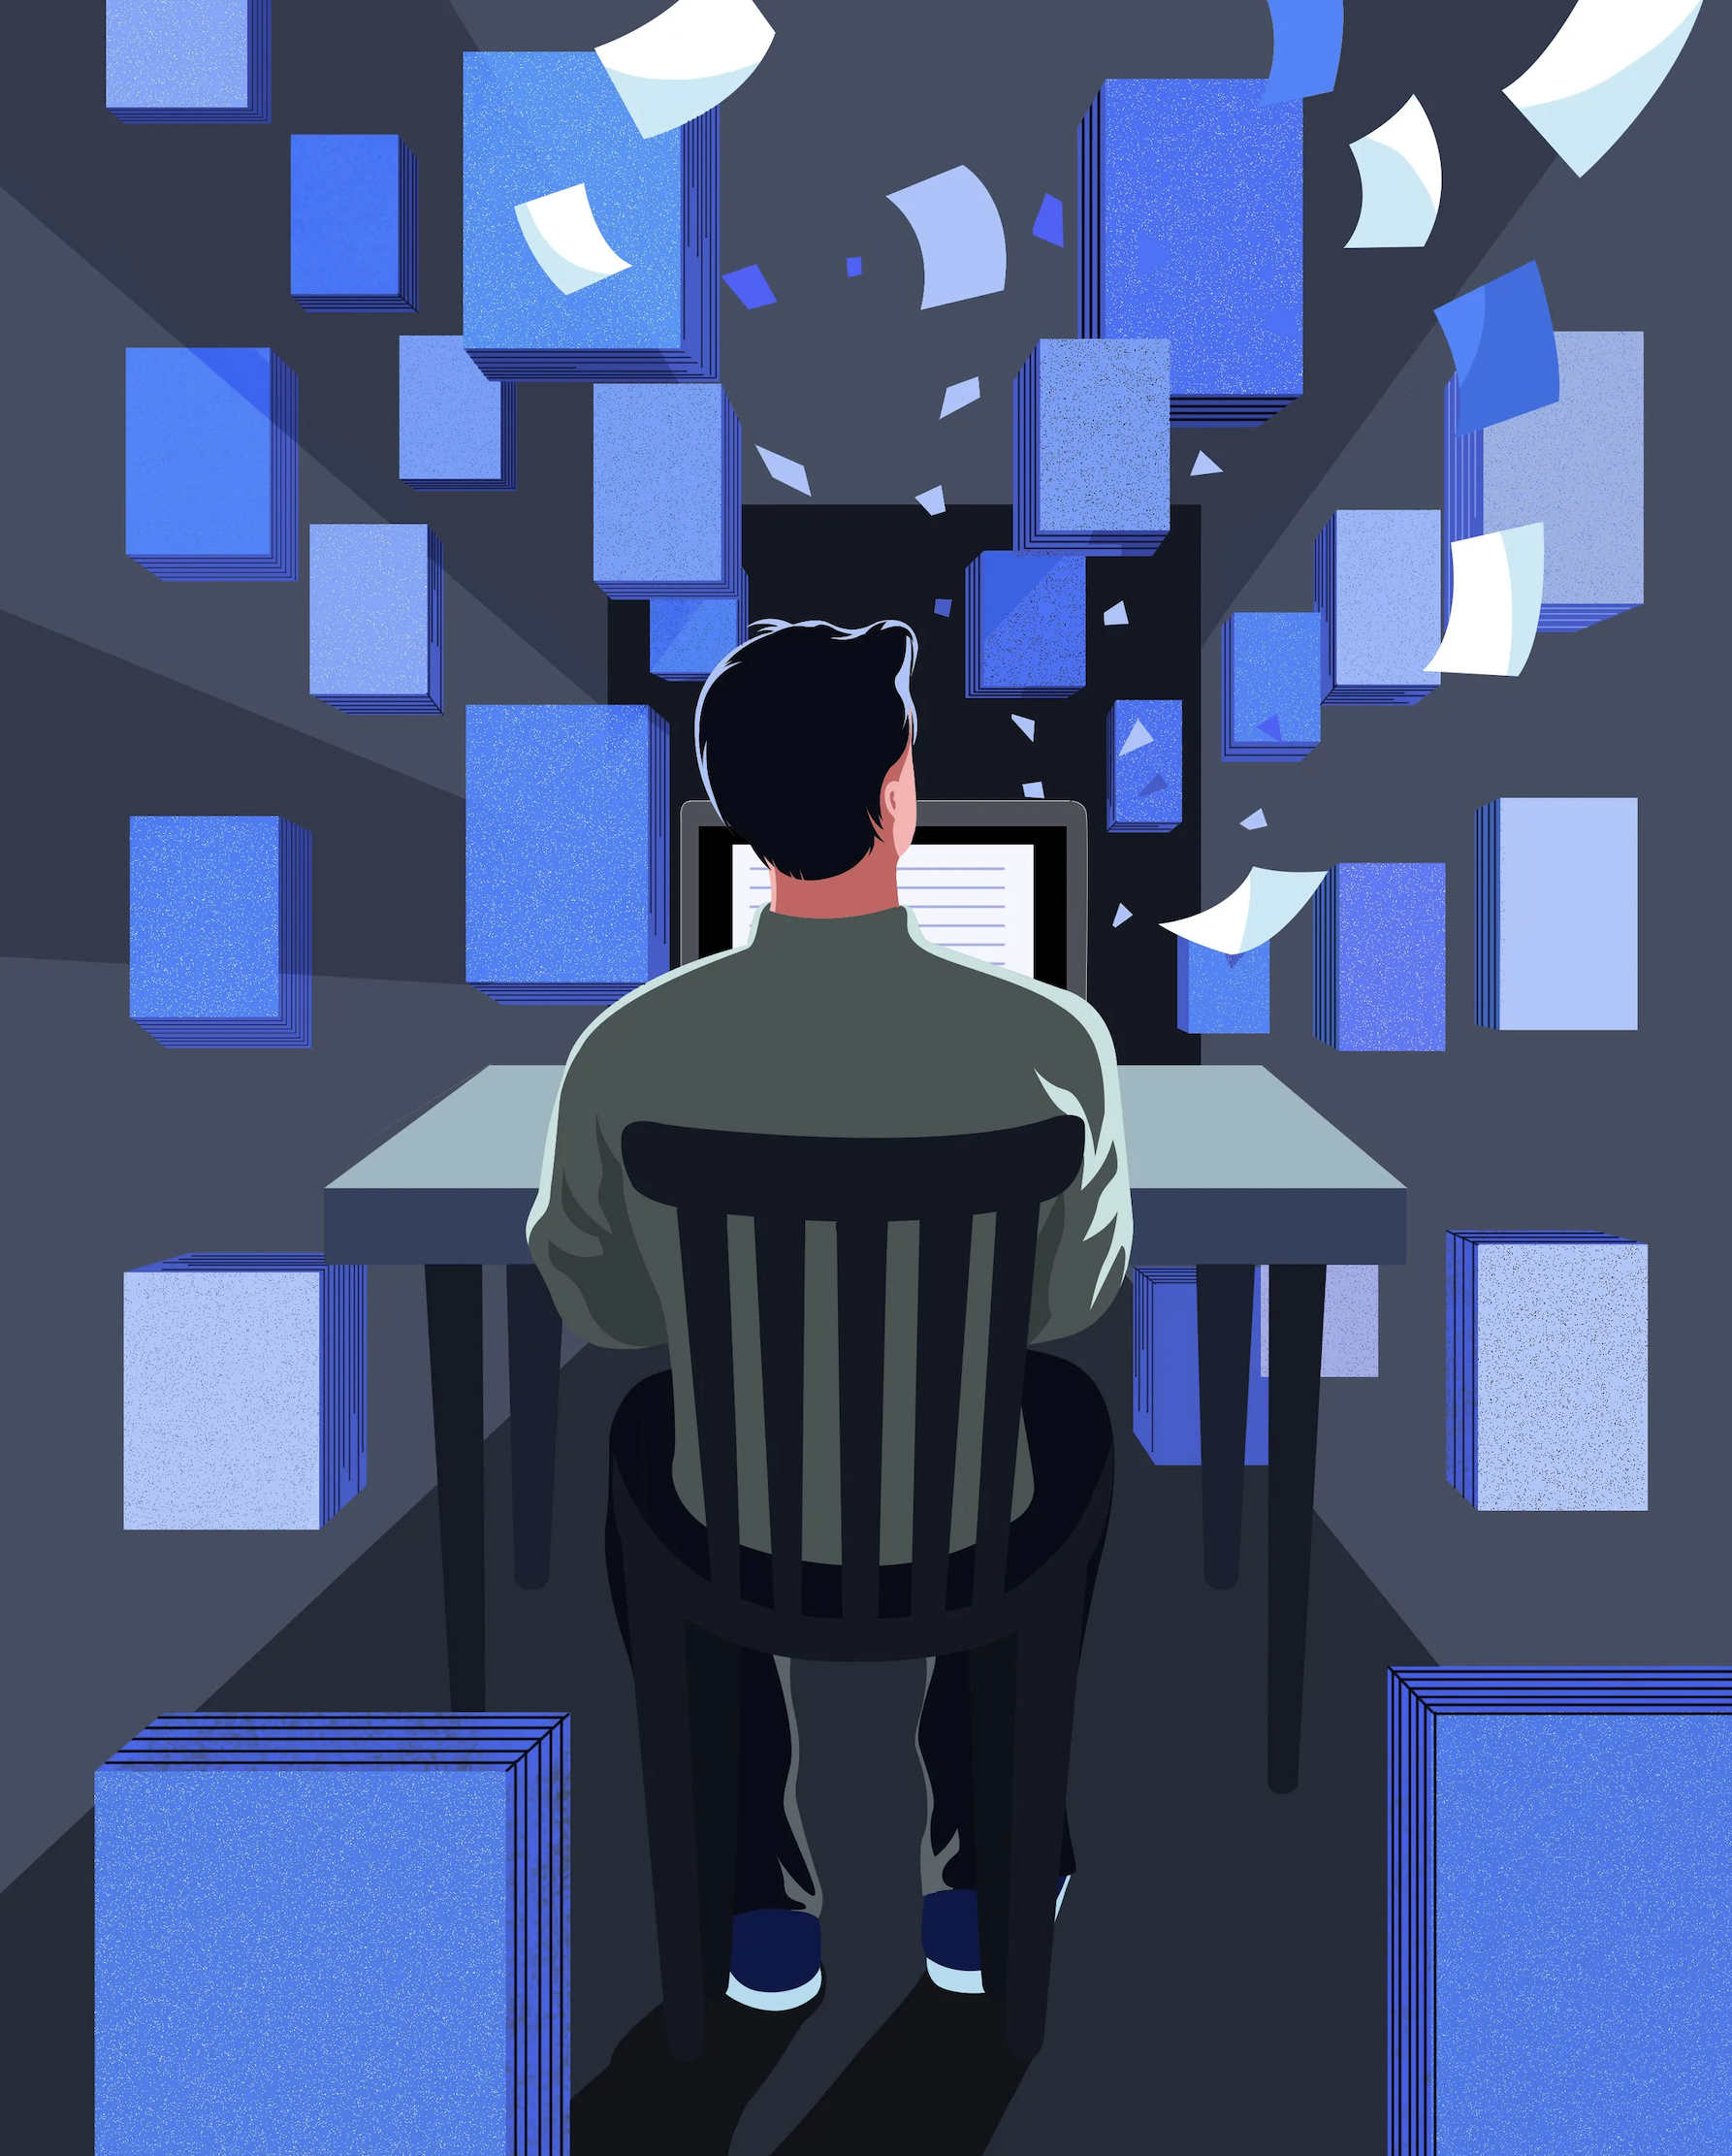
\includegraphics[width=0.35\textwidth]{figures/sample-ai.png}
%   \caption{\href{https://www.newyorker.com/culture/cultural-comment/the-computers-are-getting-better-at-writing}{The Computers Are Getting Better at Writing (The NewYorker)\sm{We don't need this figure, I would remove, you got several comments on this. definitely remove for CHI submission}}}
%   \label{fig:teaser}
% \end{teaserfigure}

\received{20 February 2007}
\received[revised]{12 March 2009}
\received[accepted]{5 June 2009}


\maketitle

% \newcommand{\optimality}{{\mathcal O}}
\newcommand{\voptimality}{{\mathcal O}}
\newcommand{\penv}{p_{\text{env}}}
\newcommand{\done}{\text{done}}
\newcommand{\stopgrad}{\text{sg}}
%\newcommand{\snr}{\text{SNR}_{\infparams}}
\newcommand{\snr}{R}
\newcommand{\Jac}{\text{Jac}}
\newcommand{\icdf}{\text{icdf}}

\newcommand{\missing}{\text{mis}}
\newcommand{\observed}{\text{obs}}

\newcommand{\hmu}{\vh_{\vmu}}
\newcommand{\hsigma}{\vh_{\vSigma}}

\newcommand{\low}{\text{low}}
\newcommand{\high}{\text{high}}

\def\ceil#1{\lceil #1 \rceil}
\def\floor#1{\lfloor #1 \rfloor}
\def\1{\bm{1}}

\def\eps{{\epsilon}}

\newcommand{\Lsimple}{L_{\text{simple}}}
\newcommand{\oalpha}{\overline{\alpha}}

\newcommand{\env}{\calE}

\newcommand{\flowvx}{\vx}
\newcommand{\flowx}{x}
\newcommand{\flowvu}{\vu}
\newcommand{\flowu}{u}

\newcommand{\todokevin}[1]{{\color{green}{TODO(kevin):#1}}}
\newcommand{\balaji}[1]{{\color{red}{TODO(balaji):#1}}}
\newcommand{\notes}[1]{{\color{red}{#1}}}
\newcommand{\vcoupling}{\hat{\mathbf{f}}}
\newcommand{\coupling}{\hat{f}}
\newcommand{\scalarbijection}{h}
% KL divergence
\newcommand{\kl}[2]{D_{\mathrm{KL}}\left[\,#1\,\|\,#2\,\right]}
% Densities
\newcommand{\createDensityWithSub}[2]{{#1}_{\mathrm{#2}}}
\newcommand{\pz}{\createDensityWithSub{p}{z}}
\newcommand{\pzprime}{\createDensityWithSub{p}{z'}}
\newcommand{\px}{\createDensityWithSub{p}{x}}


\newcommand{\fdyn}{f^{\text{dyn}}}
\newcommand{\fobs}{f^{\text{obs}}}
\newcommand{\freward}{f^{\text{R}}}

\newcommand{\ESS}{\text{ESS}}

% LDA
\newcommand{\Ntopics}{{N_z}}
\newcommand{\Nwords}{{N_w}}


%https://www.overleaf.com/learn/latex/Mathematical_fonts
%\prescript{\mathrm t}{}{A},

%https://tex.stackexchange.com/questions/121865/nameref-how-to-display-section-name-and-its-number
\newcommand*{\fullref}[1]{\hyperref[{#1}]{\cref{#1} (\nameref*{#1})}}
%\newcommand*{\fullref}[1]{\hyperref[{#1}]{\autoref*{#1} (\nameref*{#1})}}

\newcommand{\eat}[1]{}
\newcommand{\new}{\text{new}}

%https://tex.stackexchange.com/questions/246/when-should-i-use-input-vs-include
\newcommand{\myinclude}[1]{\include{#1}}
%\newcommand{\myinclude}[1]{\input{#1}} 

\mathchardef\mhyphen="2D % Define a "math hyphen"
\mathchardef\mdash="2D % Define a "math hyphen"

\newcommand{\ie}{\emph{i.e.}}
\newcommand{\condition}{\,|\,}
\newcommand{\eg}{\emph{e.g.}}
\newcommand{\bo}{\mathbf{o}}
\newcommand{\bx}{\mathbf{x}}
\newcommand{\by}{\mathbf{y}}
\newcommand{\bc}{\mathbf{c}}

\newcommand{\colvec}[1]{\ensuremath{\begin{pmatrix} #1 \end{pmatrix}}}
\newcommand{\myvec}[1]{\mathbf{#1}}
\newcommand{\myvecsym}[1]{\boldsymbol{#1}}
%\newcommand{\myvecsym}[1]{\bm{#1}}
\newcommand{\mytensor}[1]{\mathbf{\tilde{#1}}}

%\newcommand{\prior}[1]{\underline{#1}}
%\newcommand{\post}[1]{\overline{#1}}

%\newcommand\smileacc[1]{\overset{\adjustedaccent{\smallsmile}}{#1}}
%\newcommand\frownacc[1]{\overset{\adjustedaccent{\smallfrown}}{#1}}
%\newcommand\smileacc[1]{\overset{\smallsmile}{#1}}
%\newcommand\frownacc[1]{\overset{\smallfrown}{#1}}

%https://tex.stackexchange.com/questions/194798/change-vertical-space-in-overset


\makeatletter
\newcommand{\oset}[3][-0.3ex]{%
  \mathrel{\mathop{#3}\limits^{
    \vbox to#1{\kern-4\ex@
    \hbox{$\scriptstyle#2$}\vss}}}}
\makeatother
\newcommand\smileacc[1]{\oset{\smallsmile}{#1}}
\newcommand\frownacc[1]{\oset{\smallfrown}{#1}}

\newcommand{\priorDist}{\pi_0}
\newcommand{\prior}[1]{\smileacc{#1}}
\newcommand{\post}[1]{\frownacc{#1}}

\newcommand{\pseudox}{\tilde{\vx}}
\newcommand{\acqfn}{\alpha}
\newcommand{\mynew}{\mathrm{new}}
\newcommand{\myold}{\mathrm{old}}
\newcommand{\mymin}{\mathrm{min}}
\newcommand{\mymax}{\mathrm{max}}
\newcommand{\rnn}{\mathrm{rnn}}

\newcommand{\acceptance}{A}
\newcommand{\centered}[1]{{#1}_c}

\newcommand{\vmask}{\vs}
\newcommand{\mask}{s}

\newcommand{\vauxvar}{\vv}
\newcommand{\auxvar}{v}

\newcommand{\SSeff}{S_{\text{eff}}}
\newcommand{\SSmin}{S_{\text{min}}}

% Numbers
\newcommand{\vzero}{\myvecsym{0}}
\newcommand{\vone}{\myvecsym{1}}


% Greek https://www.latex-tutorial.com/symbols/greek-alphabet/
\newcommand{\valpha}{\myvecsym{\alpha}}
\newcommand{\vbeta}{\myvecsym{\beta}}
\newcommand{\vchi}{\myvecsym{\chi}}
\newcommand{\vdelta}{\myvecsym{\delta}}
\newcommand{\vDelta}{\myvecsym{\Delta}}
\newcommand{\vepsilon}{\myvecsym{\epsilon}}
\newcommand{\vzeta}{\myvecsym{\zeta}}
\newcommand{\vXi}{\myvecsym{\Xi}}
\newcommand{\vell}{\myvecsym{\ell}}
\newcommand{\veta}{\myvecsym{\eta}}
%\newcommand{\vEta}{\myvecsym{\Eta}}
\newcommand{\vgamma}{\myvecsym{\gamma}}
\newcommand{\vGamma}{\myvecsym{\Gamma}}
\newcommand{\vmu}{\myvecsym{\mu}}
\newcommand{\vmut}{\myvecsym{\tilde{\mu}}}
\newcommand{\vnu}{\myvecsym{\nu}}
\newcommand{\vkappa}{\myvecsym{\kappa}}
\newcommand{\vlambda}{\myvecsym{\lambda}}
\newcommand{\vLambda}{\myvecsym{\Lambda}}
\newcommand{\vLambdaBar}{\overline{\vLambda}}
%\newcommand{\vnu}{\myvecsym{\nu}}
\newcommand{\vomega}{\myvecsym{\omega}}
\newcommand{\vOmega}{\myvecsym{\Omega}}
\newcommand{\vphi}{\myvecsym{\phi}}
\newcommand{\vvarphi}{\myvecsym{\varphi}}
\newcommand{\vPhi}{\myvecsym{\Phi}}
\newcommand{\vpi}{\myvecsym{\pi}}
\newcommand{\vPi}{\myvecsym{\Pi}}
\newcommand{\vpsi}{\myvecsym{\psi}}
\newcommand{\vPsi}{\myvecsym{\Psi}}
\newcommand{\vrho}{\myvecsym{\rho}}
\newcommand{\vtheta}{\myvecsym{\theta}}
\newcommand{\vthetat}{\myvecsym{\tilde{\theta}}}
\newcommand{\vTheta}{\myvecsym{\Theta}}
\newcommand{\vsigma}{\myvecsym{\sigma}}
\newcommand{\vSigma}{\myvecsym{\Sigma}}
\newcommand{\vSigmat}{\myvecsym{\tilde{\Sigma}}}
\newcommand{\vsigmoid}{\vsigma}
\newcommand{\vtau}{\myvecsym{\tau}}
\newcommand{\vxi}{\myvecsym{\xi}}


% Lower Roman (Vectors)
\newcommand{\va}{\myvec{a}}
\newcommand{\vb}{\myvec{b}}
\newcommand{\vBt}{\myvec{\tilde{B}}}
\newcommand{\vc}{\myvec{c}}
\newcommand{\vct}{\myvec{\tilde{c}}}
\newcommand{\vd}{\myvec{d}}
\newcommand{\ve}{\myvec{e}}
\newcommand{\vf}{\myvec{f}}
\newcommand{\vg}{\myvec{g}}
\newcommand{\vh}{\myvec{h}}
%\newcommand{\myvh}{\myvec{h}}
\newcommand{\vi}{\myvec{i}}
\newcommand{\vj}{\myvec{j}}
\newcommand{\vk}{\myvec{k}}
\newcommand{\vl}{\myvec{l}}
\newcommand{\vm}{\myvec{m}}
\newcommand{\vn}{\myvec{n}}
\newcommand{\vo}{\myvec{o}}
\newcommand{\vp}{\myvec{p}}
\newcommand{\vq}{\myvec{q}}
\newcommand{\vr}{\myvec{r}}
\newcommand{\vs}{\myvec{s}}
\newcommand{\vt}{\myvec{t}}
\newcommand{\vu}{\myvec{u}}
\newcommand{\vv}{\myvec{v}}
\newcommand{\vw}{\myvec{w}}
\newcommand{\vws}{\vw_s}
\newcommand{\vwt}{\myvec{\tilde{w}}}
\newcommand{\vWt}{\myvec{\tilde{W}}}
\newcommand{\vwh}{\hat{\vw}}
\newcommand{\vx}{\myvec{x}}
%\newcommand{\vx}{\myvec{x}}
\newcommand{\vxt}{\myvec{\tilde{x}}}
\newcommand{\vy}{\myvec{y}}
\newcommand{\vyt}{\myvec{\tilde{y}}}
\newcommand{\vz}{\myvec{z}}
%\newcommand{\vzt}{\myvec{\tilde{z}}}


% Elements of vectors
\def\evalpha{{\alpha}}
\def\evbeta{{\beta}}
\def\evepsilon{{\epsilon}}
\def\evlambda{{\lambda}}
\def\evomega{{\omega}}
\def\evmu{{\mu}}
\def\evpsi{{\psi}}
\def\evsigma{{\sigma}}
\def\evtheta{{\theta}}
\def\eva{{a}}
\def\evb{{b}}
\def\evc{{c}}
\def\evd{{d}}
\def\eve{{e}}
\def\evf{{f}}
\def\evg{{g}}
\def\evh{{h}}
\def\evi{{i}}
\def\evj{{j}}
\def\evk{{k}}
\def\evl{{l}}
\def\evm{{m}}
\def\evn{{n}}
\def\evo{{o}}
\def\evp{{p}}
\def\evq{{q}}
\def\evr{{r}}
\def\evs{{s}}
\def\evt{{t}}
\def\evu{{u}}
\def\evv{{v}}
\def\evw{{w}}
\def\evx{{x}}
\def\evy{{y}}
\def\evz{{z}}

% Upper Roman (Matrices)
\newcommand{\vA}{\myvec{A}}
\newcommand{\vB}{\myvec{B}}
\newcommand{\vC}{\myvec{C}}
\newcommand{\vD}{\myvec{D}}
\newcommand{\vE}{\myvec{E}}
\newcommand{\vF}{\myvec{F}}
\newcommand{\vG}{\myvec{G}}
\newcommand{\vH}{\myvec{H}}
\newcommand{\vI}{\myvec{I}}
\newcommand{\vJ}{\myvec{J}}
\newcommand{\vK}{\myvec{K}}
\newcommand{\vL}{\myvec{L}}
\newcommand{\vM}{\myvec{M}}
\newcommand{\vMt}{\myvec{\tilde{M}}}
\newcommand{\vN}{\myvec{N}}
\newcommand{\vO}{\myvec{O}}
\newcommand{\vP}{\myvec{P}}
\newcommand{\vQ}{\myvec{Q}}
\newcommand{\vR}{\myvec{R}}
\newcommand{\vS}{\myvec{S}}
\newcommand{\vT}{\myvec{T}}
\newcommand{\vU}{\myvec{U}}
\newcommand{\vV}{\myvec{V}}
\newcommand{\vW}{\myvec{W}}
\newcommand{\vX}{\myvec{X}}
%\newcommand{\vXs}{\vX_{\vs}}
\newcommand{\vXs}{\vX_{s}}
\newcommand{\vXt}{\myvec{\tilde{X}}}
\newcommand{\vY}{\myvec{Y}}
\newcommand{\vZ}{\myvec{Z}}
\newcommand{\vZt}{\myvec{\tilde{Z}}}
\newcommand{\vzt}{\myvec{\tilde{z}}}


% Matrix
\def\mA{{\bm{A}}}
\def\mB{{\bm{B}}}
\def\mC{{\bm{C}}}
\def\mD{{\bm{D}}}
\def\mE{{\bm{E}}}
\def\mF{{\bm{F}}}
\def\mG{{\bm{G}}}
\def\mH{{\bm{H}}}
\def\mI{{\bm{I}}}
\def\mJ{{\bm{J}}}
\def\mK{{\bm{K}}}
\def\mL{{\bm{L}}}
\def\mM{{\bm{M}}}
\def\mN{{\bm{N}}}
\def\mO{{\bm{O}}}
\def\mP{{\bm{P}}}
\def\mQ{{\bm{Q}}}
\def\mR{{\bm{R}}}
\def\mS{{\bm{S}}}
\def\mT{{\bm{T}}}
\def\mU{{\bm{U}}}
\def\mV{{\bm{V}}}
\def\mW{{\bm{W}}}
\def\mX{{\bm{X}}}
\def\mY{{\bm{Y}}}
\def\mZ{{\bm{Z}}}
\def\mBeta{{\bm{\beta}}}
\def\mPhi{{\bm{\Phi}}}
\def\mLambda{{\bm{\Lambda}}}
\def\mSigma{{\bm{\Sigma}}}


% tensors
%\newcommand{\tX}{\mytensor{X}}
%\newcommand{\tY}{\mytensor{Y}}
%\newcommand{\tZ}{\mytensor{Z}}
%\newcommand{\tW}{\mytensor{W}}


% Tensor
\DeclareMathAlphabet{\mathsfit}{\encodingdefault}{\sfdefault}{m}{sl}
\SetMathAlphabet{\mathsfit}{bold}{\encodingdefault}{\sfdefault}{bx}{n}
\newcommand{\tens}[1]{\bm{\mathsfit{#1}}}
\def\tA{{\tens{A}}}
\def\tB{{\tens{B}}}
\def\tC{{\tens{C}}}
\def\tD{{\tens{D}}}
\def\tE{{\tens{E}}}
\def\tF{{\tens{F}}}
\def\tG{{\tens{G}}}
\def\tH{{\tens{H}}}
\def\tI{{\tens{I}}}
\def\tJ{{\tens{J}}}
\def\tK{{\tens{K}}}
\def\tL{{\tens{L}}}
\def\tM{{\tens{M}}}
\def\tN{{\tens{N}}}
\def\tO{{\tens{O}}}
\def\tP{{\tens{P}}}
\def\tQ{{\tens{Q}}}
\def\tR{{\tens{R}}}
\def\tS{{\tens{S}}}
\def\tT{{\tens{T}}}
\def\tU{{\tens{U}}}
\def\tV{{\tens{V}}}
\def\tW{{\tens{W}}}
\def\tX{{\tens{X}}}
\def\tY{{\tens{Y}}}
\def\tZ{{\tens{Z}}}


% Graph
\def\gA{{\mathcal{A}}}
\def\gB{{\mathcal{B}}}
\def\gC{{\mathcal{C}}}
\def\gD{{\mathcal{D}}}
\def\gE{{\mathcal{E}}}
\def\gF{{\mathcal{F}}}
\def\gG{{\mathcal{G}}}
\def\gH{{\mathcal{H}}}
\def\gI{{\mathcal{I}}}
\def\gJ{{\mathcal{J}}}
\def\gK{{\mathcal{K}}}
\def\gL{{\mathcal{L}}}
\def\gM{{\mathcal{M}}}
\def\gN{{\mathcal{N}}}
\def\gO{{\mathcal{O}}}
\def\gP{{\mathcal{P}}}
\def\gQ{{\mathcal{Q}}}
\def\gR{{\mathcal{R}}}
\def\gS{{\mathcal{S}}}
\def\gT{{\mathcal{T}}}
\def\gU{{\mathcal{U}}}
\def\gV{{\mathcal{V}}}
\def\gW{{\mathcal{W}}}
\def\gX{{\mathcal{X}}}
\def\gY{{\mathcal{Y}}}
\def\gZ{{\mathcal{Z}}}

% Sets
\def\sA{{\mathbb{A}}}
\def\sB{{\mathbb{B}}}
\def\sC{{\mathbb{C}}}
\def\sD{{\mathbb{D}}}
% Don't use a set called E, because this would be the same as our symbol
% for expectation.
\def\sF{{\mathbb{F}}}
\def\sG{{\mathbb{G}}}
\def\sH{{\mathbb{H}}}
\def\sI{{\mathbb{I}}}
\def\sJ{{\mathbb{J}}}
\def\sK{{\mathbb{K}}}
\def\sL{{\mathbb{L}}}
\def\sM{{\mathbb{M}}}
\def\sN{{\mathbb{N}}}
\def\sO{{\mathbb{O}}}
\def\sP{{\mathbb{P}}}
\def\sQ{{\mathbb{Q}}}
\def\sR{{\mathbb{R}}}
\def\sS{{\mathbb{S}}}
\def\sT{{\mathbb{T}}}
\def\sU{{\mathbb{U}}}
\def\sV{{\mathbb{V}}}
\def\sW{{\mathbb{W}}}
\def\sX{{\mathbb{X}}}
\def\sY{{\mathbb{Y}}}
\def\sZ{{\mathbb{Z}}}

% Entries of a matrix
\def\emLambda{{\Lambda}}
\def\emA{{A}}
\def\emB{{B}}
\def\emC{{C}}
\def\emD{{D}}
\def\emE{{E}}
\def\emF{{F}}
\def\emG{{G}}
\def\emH{{H}}
\def\emI{{I}}
\def\emJ{{J}}
\def\emK{{K}}
\def\emL{{L}}
\def\emM{{M}}
\def\emN{{N}}
\def\emO{{O}}
\def\emP{{P}}
\def\emQ{{Q}}
\def\emR{{R}}
\def\emS{{S}}
\def\emT{{T}}
\def\emU{{U}}
\def\emV{{V}}
\def\emW{{W}}
\def\emX{{X}}
\def\emY{{Y}}
\def\emZ{{Z}}
\def\emSigma{{\Sigma}}

% entries of a tensor
% Same font as tensor, without \bm wrapper
\newcommand{\etens}[1]{\mathsfit{#1}}
\def\etLambda{{\etens{\Lambda}}}
\def\etA{{\etens{A}}}
\def\etB{{\etens{B}}}
\def\etC{{\etens{C}}}
\def\etD{{\etens{D}}}
\def\etE{{\etens{E}}}
\def\etF{{\etens{F}}}
\def\etG{{\etens{G}}}
\def\etH{{\etens{H}}}
\def\etI{{\etens{I}}}
\def\etJ{{\etens{J}}}
\def\etK{{\etens{K}}}
\def\etL{{\etens{L}}}
\def\etM{{\etens{M}}}
\def\etN{{\etens{N}}}
\def\etO{{\etens{O}}}
\def\etP{{\etens{P}}}
\def\etQ{{\etens{Q}}}
\def\etR{{\etens{R}}}
\def\etS{{\etens{S}}}
\def\etT{{\etens{T}}}
\def\etU{{\etens{U}}}
\def\etV{{\etens{V}}}
\def\etW{{\etens{W}}}
\def\etX{{\etens{X}}}
\def\etY{{\etens{Y}}}
\def\etZ{{\etens{Z}}}


\newcommand{\bbI}{\mathbb{I}}
\newcommand{\bbL}{\mathbb{L}}
\newcommand{\bbM}{\mathbb{M}}
\newcommand{\bbP}{\mathbb{P}}
\newcommand{\bbQ}{\mathbb{Q}}
\newcommand{\bbS}{\mathbb{S}}



%\newcommand{\mymathcal}[1]{\pazocal{#1}}
\newcommand{\mymathcal}[1]{\mathcal{#1}}

\newcommand{\calA}{\mymathcal{A}}
\newcommand{\calB}{\mymathcal{B}}
\newcommand{\calC}{\mymathcal{C}}
\newcommand{\calD}{{\mymathcal{D}}}
\newcommand{\calDx}{\calD_x}
\newcommand{\calE}{\mymathcal{E}}
\newcommand{\cale}{{\cal e}}
\newcommand{\calF}{\mymathcal{F}}
\newcommand{\calG}{\mymathcal{G}}
\newcommand{\calH}{\mymathcal{H}}
\newcommand{\calHX}{{\calH}_X}
\newcommand{\calHy}{{\calH}_y}
\newcommand{\calI}{\mymathcal{I}}
\newcommand{\calJ}{\mymathcal{J}}
\newcommand{\calK}{\mymathcal{K}}
\newcommand{\calL}{\mymathcal{L}}
\newcommand{\calM}{\mymathcal{M}}
\newcommand{\calN}{\mymathcal{N}}
\newcommand{\caln}{{\cal n}}
\newcommand{\calNP}{\mymathcal{NP}}
\newcommand{\calO}{\mymathcal{O}}
\newcommand{\calMp}{\calM^+}
\newcommand{\calMm}{\calM^-}
\newcommand{\calMo}{\calM^o}
\newcommand{\Ctest}{C_*}
\newcommand{\calP}{\mymathcal{P}}
\newcommand{\calq}{{\cal q}}
\newcommand{\calQ}{\mymathcal{Q}}
\newcommand{\calR}{\mymathcal{R}}
\newcommand{\calS}{\mymathcal{S}}
\newcommand{\calSstar}{\calS_*}
\newcommand{\calT}{\mymathcal{T}}
\newcommand{\calU}{\mymathcal{U}}
\newcommand{\calV}{\mymathcal{V}}
\newcommand{\calW}{\mymathcal{W}}
\newcommand{\calv}{{\cal v}}
\newcommand{\calX}{\mymathcal{X}}
\newcommand{\calY}{\mymathcal{Y}}
\newcommand{\calZ}{\mymathcal{Z}}


%%%%%%%

\newcommand{\betadist}{\mathrm{Beta}}
\newcommand{\Betadist}{\mathrm{Beta}}
\newcommand{\bernoulli}{\mathrm{Ber}}
\newcommand{\Ber}{\mathrm{Ber}}
\newcommand{\BB}{\mathrm{BetaBinom}}
\newcommand{\Binom}{\mathrm{Bin}}
\newcommand{\BinoDist}{\mathrm{Bin}}
\newcommand{\NegBinom}{\mathrm{NegBinom}}
\newcommand{\binomdist}{\mathrm{Bin}}
%\newcommand{\cauchy}{\mathrm{Cauchy}}
\newcommand{\cauchy}{\mathcal{C}}
\newcommand{\Cauchy}{\cauchy}
\newcommand{\DE}{\mathrm{DE}}
\newcommand{\DP}{\mathrm{DP}}
\newcommand{\PYP}{\mathrm{PYP}}
\newcommand{\Dir}{\mathrm{Dir}}
%\newcommand{\discrete}{\mathrm{Discrete}}
\newcommand{\erlang}{\mathrm{Erlang}}
\newcommand{\expdist}{\mathrm{Expon}}
\newcommand{\expon}{\mathrm{Expon}}
\newcommand{\expfam}{\mathrm{Expfam}}
\newcommand{\Expfam}{\mathrm{Expfam}}
\newcommand{\gammadist}{\mathrm{Ga}}
\newcommand{\Ga}{\mathrm{Ga}}
\newcommand{\GDP}{\mathrm{GDP}}
\newcommand{\GP}{\mathrm{GP}}
\newcommand{\GEM}{\mathrm{GEM}}
\newcommand{\gauss}{\mathcal{N}}
\newcommand{\loggauss}{\mathcal{LN}}
\newcommand{\matrixgauss}{\mathcal{MN}}
\newcommand{\MNIW}{\mathrm{MNIW}}
\newcommand{\circulargauss}{\mathrm{vMF}}
\newcommand{\gausscan}{\mathcal{N}_c}
\newcommand{\geom}{\mathrm{Geom}}
%\newcommand{\halfCauchy}{\mathrm{HalfCauchy}}
\newcommand{\halfCauchy}{\mathcal{C}_+}
\newcommand{\HalfCauchy}{\halfCauchy}
\newcommand{\halfcauchy}{\halfCauchy}
\newcommand{\halfNormal}{\mathcal{N}_+}
%\newcommand{\halfNormal}{\mathrm{HalfNormal}}
\newcommand{\horseshoe}{\mathrm{HS}}
%\newcommand{\IG}{\mathrm{InvGam}}
\newcommand{\IG}{\mathrm{IG}}
\newcommand{\IGauss}{\mathrm{InvGauss}}
%\newcommand{\invchi}{\chi^{-2}}
\newcommand{\invchisq}{\chi^{-2}}
\newcommand{\IW}{\mathrm{IW}}
\newcommand{\Laplace}{\mathrm{Laplace}}
\newcommand{\laplace}{\mathrm{Laplace}} % Laplace distribution
\newcommand{\LKJ}{\mathrm{LKJ}}
\newcommand{\LKJchol}{\mathrm{LKJchol}}
\newcommand{\logisticdist}{\mathrm{Logistic}}
%\newcommand{\Mu}{\mathrm{Mu}}
\newcommand{\Mu}{\mathcal{M}}
\newcommand{\Multi}{\Mu}
\newcommand{\NIX}{NI\chi^2}
\newcommand{\NJ}{\mathrm{NJ}}
\newcommand{\GIX}{NI\chi^2}
\newcommand{\NIG}{\mathrm{NIG}}
\newcommand{\GIG}{\mathrm{NIG}}
\newcommand{\NIW}{\mathrm{NIW}}
\newcommand{\GIW}{\mathrm{NIW}}
\newcommand{\GT}{{\mathrm{GT}}}
%\newcommand{\MVNIW}{\mathrm{MVNIW}}
\newcommand{\MVNIW}{\mathrm{NIW}}
\newcommand{\NW}{\mathrm{NWI}}
\newcommand{\NWI}{\mathrm{NWI}}
%\newcommand{\MVNIG}{\mathrm{MVNIG}}
\newcommand{\MVNIG}{\mathrm{NIG}}
\newcommand{\NGdist}{\mathrm{NG}}
\newcommand{\prob}{p}
\newcommand{\Plaw}{\mathbb{P}}
\newcommand{\Poi}{\mathrm{Poi}}
%\newcommand{\softmax}{\calS}
\newcommand{\softmax}{\mathrm{softmax}}
%\newcommand{\softmax}{\vsigma}
\newcommand{\Student}{\mathcal{T}}
\newcommand{\student}{\mathcal{T}}
\newcommand{\unif}{\mathrm{Unif}}
\newcommand{\Unif}{\unif}
\newcommand{\uniform}{\unif}
\newcommand{\Wishart}{\mathrm{Wi}}
\newcommand{\Wi}{\mathrm{Wi}}
\newcommand{\poissondist}{\mathrm{Poisson}}
\newcommand{\dirichletdist}{\mathrm{Dir}}

\newcommand{\cat}{\mathrm{Cat}}
%\newcommand{\cat}{\Mu}
\newcommand{\Cat}{\cat}
\newcommand{\discrete}{\cat}
\newcommand{\Discrete}{\cat}

\newcommand{\attn}{\mathrm{Attn}}
\newcommand{\atten}{\attn}
\newcommand{\attnWeights}{\alpha}
\newcommand{\attenWeights}{\attnWeights}
\newcommand{\attnScore}{a}
\newcommand{\attenScore}{\attnScore}

\newcommand{\LOO}{\mathrm{LOO}}
%%%%%%%%%%%%%%%%%%%%%%%%%%%%%%%%%%%%%%%%%%%%%%%%


\newcommand{\cbar}{\overline{c}}
\newcommand{\vcbar}{\overline{\vc}}
\newcommand{\fbar}{\overline{f}}
\newcommand{\myhbar}{\overline{h}}
\newcommand{\xmybar}{\overline{x}}
\newcommand{\ybar}{\overline{y}}
\newcommand{\zbar}{\overline{z}}
\newcommand{\vAbar}{\overline{\vA}}
\newcommand{\vBbar}{\overline{\vB}}
\newcommand{\vCbar}{\overline{\vC}}
\newcommand{\vxbar}{\overline{\vx}}
\newcommand{\vXbar}{\overline{\vX}}
\newcommand{\vybar}{\overline{\vy}}
\newcommand{\vYbar}{\overline{\vY}}
\newcommand{\vzbar}{\overline{\vz}}
\newcommand{\vZbar}{\overline{\vZ}}
\newcommand{\xbar}{\overline{x}}
\newcommand{\wbar}{\overline{w}}
\newcommand{\Xbar}{\overline{X}}
\newcommand{\Ybar}{\overline{Y}}
\newcommand{\Gbar}{\overline{G}}
\newcommand{\Jbar}{\overline{J}}
\newcommand{\Lbar}{\overline{\ell}}
\newcommand{\Nbar}{\overline{N}}
%\newcommand{\Qbar}{\overline{Q}}
\newcommand{\Qbar}{\overline{Q}}
\newcommand{\Abar}{\overline{A}}
\newcommand{\Tbar}{\overline{T}}
\newcommand{\Sbar}{\overline{S}}
\newcommand{\vSbar}{\overline{\vS}}
\newcommand{\Rbar}{\overline{R}}

\newcommand{\vtaubar}{\overline{\vtau}}
\newcommand{\vtbar}{\overline{\vt}}
\newcommand{\vsbar}{\overline{\vs}}
\newcommand{\mubar}{\overline{\mu}}
\newcommand{\phibar}{\overline{\phi}}



\newcommand{\lr}{\eta}
\newcommand{\stepsize}{\lr}
\newcommand{\momentum}{\gamma}
\newcommand{\dummy}{\mathrm{dummy}}
\newcommand{\onehot}{\mathrm{one}\mhyphen\mathrm{hot}}
%\newcommand{\onehot}{\mathrm{one-hot}}
\newcommand{\encode}{\mathrm{enc}}
\newcommand{\decode}{\mathrm{dec}}
\newcommand{\mydigamma}{\psi}

\newcommand{\AEencoder}{f_e}
\newcommand{\AEdecoder}{f_d}
\newcommand{\encoder}{e}
\newcommand{\backcoder}{b}
\newcommand{\decoder}{d}
\newcommand{\marginal}{m}


%\newcommand{\Wgen}{\vW_{\mathrm{gen}}}
%\newcommand{\Wrec}{\vW_{\mathrm{rec}}}

%https://www.overleaf.com/learn/latex/Theorems_and_proofs

%https://tex.stackexchange.com/questions/45355/theorem-numbering-as-chapter-section-subsection-theorem-number
\newtheorem{thm}{Theorem}[section]
\newtheorem{lem}{Lemma}[section]
\newtheorem{cor}{Corollary}[section]
\newtheorem{defn}{Definition}[section]

%\newenvironment{mythm}{{\bf Theorem}}{}
%\newenvironment{myproof}{{\bf Proof}}{}


\newcommand{\eos}{\text{\em{eos}}\xspace}
%\newcommand{\eos}{\langle /s \rangle}
\newcommand{\bos}{\text{\em{bos}}\xspace}
%\newcommand{\bos}{\langle s \rangle}
\newcommand{\pad}{\mathrm{<pad>}}
\newcommand{\unk}{\mathrm{<unk>}}

\newcommand{\unknown}{\vz} % state of nature

% make qed symbol a solid square
%\renewcommand{\qed}{\mbox{$\hrulefill \blacksquare $}}

%http://jblevins.org/notes/latex#independence
\newcommand\independent{\protect\mathpalette{\protect\independenT}{\perp}} 
\def\independenT#1#2{\mathrel{\rlap{$#1#2$}\mkern2mu{#1#2}}}


%http://imaging.mrc-cbu.cam.ac.uk/statswiki/TexTips
\newcommand{\argmax}{\operatornamewithlimits{argmax}}
\newcommand{\argmin}{\operatornamewithlimits{argmin}}

%\DeclareMathOperator*{\argmax}{arg\,max}
%\DeclareMathOperator*{\argmin}{arg\,min}

%\DeclareMathOperator{\sign}{sign}
%\DeclareMathOperator{\Tr}{Tr}
\let\ab\allowbreak

\newcommand{\todo}[1]{\textbf{TODO: #1}}
\newcommand{\todol}[1]{\textcolor{blue}{\textbf{LL: #1}}}

\newcommand{\reconstruct}[1]{r({#1})}
\newcommand{\recon}{r}
\newcommand{\act}{\vz}
\newcommand{\actScalar}{z}
\newcommand{\actMat}{\vZ}
\newcommand{\preact}{\va}
\newcommand{\preactScalar}{a}
\newcommand{\preactMat}{\vA}
\newcommand{\erf}{\text{erf}}
\newcommand{\activation}{\varphi}
\newcommand{\vactivation}{\varphi}
%\newcommand{\activation}{\phi}
%\newcommand{\vactivation}{\vphi}
\newcommand{\choice}[2]{\left(\!\!\! \begin{array}{c} #1 \\ #2\end{array} \!\!\!\right)}
\newcommand{\half}{\frac{1}{2}}
\newcommand{\nicehalf}{\nicefrac{1}{2}}

\newcommand{\addeq}{\stackrel{c}{=}}
\newcommand{\pluseq}{\mathrel{+}=}
%\newcommand{\defeq}{\stackrel{\rm def}{=}}
\newcommand{\defeq}{\triangleq}
%http://tex.stackexchange.com/questions/163829/delta-equal-to-symbol
%\def\defeq{\mathrel{\ensurestackMath{\stackon[2pt]{=}{\scriptstyle\Delta}}}}

%\newcommand{\defeq}{:=}
%\newcommand{\consteq}{\stackrel{+}{=}}
\newcommand{\consteq}{\bumpeq}
%\newcommand{\real}{{\rm I\hspace{-0.2em}R}}
%\newcommand{\real}{\mathbb{R}}
\newcommand{\real}{\sR}
\newcommand{\simplex}{\mathbb{S}}
%\newcommand{\posreal}{\mathbb{R}_{>0}}
\newcommand{\posreal}{\mathbb{R}_{+}}
\newcommand{\realpos}{\posreal}
\newcommand{\nonnegreal}{\mathbb{R}_{\geq 0}}
\newcommand{\ints}{\mathbb{Z}}
%\newcommand{\natural}{\mathbb{N}}
\newcommand{\posint}{\ints_{+}} % https://proofwiki.org/wiki/Symbols:Z
\newcommand{\intpos}{\posint}
\newcommand{\posints}{\posint}
%\newcommand{\posint}{\ints_{>0}} % https://proofwiki.org/wiki/Symbols:Z
\newcommand{\nonnegint}{\ints_{\geq 0}}


\newcommand{\train}{\text{train}}
\newcommand{\test}{\text{test}}
\newcommand{\valid}{\text{valid}}
\newcommand{\meta}{\text{meta}}

\newcommand{\testNull}{\test_{\text{null}}}
\newcommand{\testObs}{\test_{\text{obs}}}
\newcommand{\testStat}{t}

%\newcommand{\indep}{\perp}
%\newcommand{\given}{\|}
\newcommand{\given}{|}
\newcommand{\indep}[2]{{#1} \perp {#2}}
\newcommand{\condindep}[3]{{#1} \perp {#2} \; | \; {#3}}
\newcommand{\condindepG}[3]{{#1} \perp_G {#2} | {#3}}
\newcommand{\condindepP}[3]{{#1} \perp_p {#2} | {#3}}
\newcommand{\depend}[2]{{#1} \not \perp {#2}}
\newcommand{\conddepend}[3]{{#1} \not \perp {#2} | {#3}}

%\newcommand{\trans}{\top}
%\newcommand{\trans}{\intercal}
\newcommand{\trans}{{\mkern-1.5mu\mathsf{T}}}
\newcommand{\transpose}[1]{{#1}^{\trans}}

\newcommand{\inv}[1]{{#1}^{-1}}

\newcommand{\ra}{\rightarrow}
\newcommand{\lra}{\leftrightarrow}
\newcommand{\Ra}{\Rightarrow}
%\newcommand{\rv}{r.v.}
\newcommand{\la}{\leftarrow}
\newcommand{\tr}{\mathrm{tr}}
\newcommand{\st}{\ \ \ \ \mathrm{s.t.} \ \ \ }
\newcommand{\myst}{\ \  \mathrm{s.t.} \ \ }
%\newcommand{\det}{\mathrm{det}}
\newcommand{\size}{\mathrm{size}}
\newcommand{\trace}{\mathrm{tr}}
\newcommand{\mle}{\mathrm{mle}}
\newcommand{\pooled}{\mathrm{pooled}}
\newcommand{\bayes}{\mathrm{bayes}}
\newcommand{\ols}{\mathrm{ols}}
\newcommand{\old}{\mathrm{old}}
\newcommand{\unb}{\mathrm{unb}}
\newcommand{\map}{\mathrm{map}}
\newcommand{\mml}{\mathrm{mml}}


\newcommand{\hparams}{\vxi}
\newcommand{\hparam}{\xi}
\newcommand{\varparams}{\vpsi}
%\newcommand{\varparams}{\vlambda}
\newcommand{\vparams}{\varparams}
\newcommand{\vparamsScalar}{\psi}
\newcommand{\vparamstheta}{\vparams_{\vtheta}}
\newcommand{\infparams}{\vphi}
\newcommand{\params}{\vtheta}
\newcommand{\param}{\theta}
\newcommand{\genparams}{\vtheta}
%\newcommand{\nparams}{{\ensuremath{N_{\theta}}\xspace}}
\newcommand{\nparams}{D}
\newcommand{\Nparams}{\nparams}
\newcommand{\nopt}{n}
\newcommand{\infnet}{f^\text{inf}_{\infparams}}
\newcommand{\gennet}{f^\text{gen}_{\genparams}}
\newcommand{\qinf}{q_{\infparams}}
\newcommand{\qinfgen}{q_{\infparams,\genparams}}
\newcommand{\qvar}{q_{\varparams}}
\newcommand{\qvarn}{q_{\varparams_n}}
\newcommand{\pgen}{p_{\params}}
\newcommand{\reparam}{g}
%\newcommand{\reparam}{\text{REPARAM}}

%\newcommand{\hvar}{\ell_{\vparams}}
%\newcommand{\hvarHat}{\hat{\ell}_{\vparams}}
%\newcommand{\hh}{\ell}
  
%\newcommand{\optvarSpace}{\mathcal{X}}
%\newcommand{\optspace}{\mathcal{X}}
%\newcommand{\optvar}{x}
%\newcommand{\optvars}{\vx}
%\newcommand{\optvarsMatrix}{\vX}
%\newcommand{\xdata}{\va}


\newcommand{\optvarSpace}{\Theta}
\newcommand{\optspace}{\Theta}
\newcommand{\optvar}{\theta}
\newcommand{\optvars}{\vtheta}
\newcommand{\optvarsScalar}{\theta}
\newcommand{\optvarsMatrix}{\vTheta}
\newcommand{\xdata}{\vx}

\newcommand{\doptvarSpace}{\calX}
\newcommand{\doptspace}{\doptvarSpace}
\newcommand{\doptvar}{x}
\newcommand{\doptvars}{\vx}

% feynman kac
\newcommand{\fkM}{M}
\newcommand{\fkMM}{\bbM}
\newcommand{\fkQQ}{\bbQ}
\newcommand{\fkPP}{\bbP}
\newcommand{\fkG}{G}
\newcommand{\fkL}{L}
\newcommand{\fkl}{l}
\newcommand{\fkernel}{\stackrel{\ra}{M}}
\newcommand{\bkernel}{\stackrel{\la}{L}}
\newcommand{\bkernelOpt}{\stackrel{\la}{M}}


% importance sampling
\newcommand{\targetDist}{\pi}
\newcommand{\targetDistSeq}{\overline{\pi}}
\newcommand{\targetUn}{\tilde{\gamma}}
\newcommand{\targetEmp}{\hat{\pi}}
\newcommand{\targetfn}{\varphi}
\newcommand{\targetFn}{\targetfn}
\newcommand{\weightsUn}{\tilde{w}}
\newcommand{\weightsNorm}{W}
\newcommand{\weightsInc}{\alpha}

\newcommand{\ancestors}{a}
\newcommand{\ancestor}{a}

\newcommand{\smcH}{\vz}
\newcommand{\smcV}{\vy}
\newcommand{\backwards}{L}
\newcommand{\forwards}{M}

\newcommand{\proposalDist}{q}
\newcommand{\proposal}{q}
\newcommand{\qproposal}{\proposal}


\newcommand{\pmodel}{p_{\vtheta}}
\newcommand{\ptrue}{p^*}
%\newcommand{\pemp}{p_{\text{data}}}
\newcommand{\pemp}{p_{\data}}
\newcommand{\qemp}{q_{\data}}
\newcommand{\ptrain}{p_{\mathrm{tr}}}
%\newcommand{\ptrain}{p_1}
\newcommand{\ptest}{p_{\mathrm{te}}}
%\newcommand{\ptest}{p_2}
\newcommand{\pdata}{\pemp}

\newcommand{\psource}{p}
\newcommand{\ptarget}{q}

%\newcommand{\priorz}{\pi}
%\newcommand{\pgen}{p_G}
%\newcommand{\pteacher}{p_t}
%\newcommand{\pstudent}{p_s}

\newcommand{\postloss}{\rho}

\newcommand{\IDAG}{IDAG\xspace}
\newcommand{\doPearl}{\mathrm{do}}
\newcommand{\ceffect}{\tau}
\newcommand{\ETT}{\text{ETT}}
\newcommand{\ATE}{\text{ATE}}
\newcommand{\CATE}{\text{CATE}}
\newcommand{\exog}{U}
\newcommand{\exogVal}{u}
\newcommand{\exogSet}{\calU}
\newcommand{\scm}{V}
\newcommand{\scmVal}{v}
\newcommand{\scmSet}{\calV}
\newcommand{\POM}{POM\xspace}


\newcommand{\outcome}{Y}
\newcommand{\outcomeVal}{y}
\newcommand{\joutcome}{\tilde{\vY}}
\newcommand{\poutcome}[1]{\outcome^{#1}} % Y_a potential outcome
\newcommand{\pout}[2]{\outcome^{#1}_{#2}} % Y_{a,i} action a, unit  i
\newcommand{\ptreat}[2]{\treatment^{#1}_{#2}} %X_{a,i} action a, unit  i


\newcommand{\covariate}{C}
\newcommand{\covariateVal}{c}
\newcommand{\forceTreatment}{F_A}
\newcommand{\treatment}{A}
\newcommand{\treatmentVal}{a}
\newcommand{\treatmentValv}{\va}
\newcommand{\observation}{Y}
\newcommand{\lconfounder}{U}
\newcommand{\lconfounderVal}{u}
\newcommand{\confounder}{X}
\newcommand{\confounderVal}{x}
\newcommand{\deconfounder}{S}
\newcommand{\deconfounderVal}{s}
\newcommand{\mediator}{M}
\newcommand{\mediatorVal}{m}
\newcommand{\instrument}{Z}
\newcommand{\instrumentVal}{z}
\newcommand{\instrumentValv}{\vz}

  

\newcommand{\dom}{\mathrm{dom}}
\newcommand{\bel}{\mathrm{bel}}
\newcommand{\dsep}{\mathrm{dsep}}
\newcommand{\sep}{\mathrm{sep}}
\newcommand{\entails}{\models}
\newcommand{\range}{\mathrm{range}}
\newcommand{\myspan}{\mathrm{span}}
\newcommand{\nullspace}{\mathrm{nullspace}}
\newcommand{\adj}{\mathrm{adj}}
%\newcommand{\pval}{\mathrm{p}-\mathrm{value}}

\newcommand{\pval}{\mathrm{pval}}
\newcommand{\pvalue}{p_v}

\newcommand{\chol}{\mathrm{chol}}
\newcommand{\supp}{\mathrm{supp}}

%\newcommand{\xrange}[1]{[#1]}  % for set, [n]
\newcommand{\xrange}[1]{\ensuremath{\{1,\ldots,#1\}}}  % for set, [n]


%\newcommand{\dim}{\mathrm{dim}}
\newcommand{\length}{\mathrm{T}}
\newcommand{\sinc}{\mathrm{sinc}}
\newcommand{\mse}{\mathrm{mse}}
%\newcommand{\pon}{\pi_0}
\newcommand{\poff}{p_0}
\newcommand{\pon}{p_1}
\newcommand{\lse}{\ensuremath{\mathrm{lse}}\xspace}
\newcommand{\soft}{\mathrm{SoftThreshold}}
\newcommand{\hard}{\mathrm{hard}}
\newcommand{\cond}{\mathrm{cond}}
\newcommand{\sign}{\mathrm{sign}}
\newcommand{\sgn}{\mathrm{sgn}}

\newcommand{\iid}{\ensuremath{\mathrm{iid}}\xspace}
\newcommand{\myiff}{\ensuremath{\mathrm{iff}}\xspace}
\newcommand{\pd}{\ensuremath{\mathrm{pd}}\xspace}
\newcommand{\psd}{\ensuremath{\mathrm{psd}}\xspace}
\newcommand{\pdf}{\ensuremath{\mathrm{pdf}}\xspace}
\newcommand{\cdf}{\ensuremath{\mathrm{cdf}}\xspace}
\newcommand{\pmf}{\ensuremath{\mathrm{pmf}}\xspace}
\newcommand{\RV}{\ensuremath{\mathrm{rv}}\xspace}
%\newcommand{\rv}{\ensuremath{\mathrm{rv}}\xspace}
\newcommand{\wrt}{\ensuremath{\mathrm{wrt}}\xspace}
\newcommand{\mywp}{\ensuremath{\mathrm{wp}}\xspace}
\newcommand{\RSS}{\ensuremath{\mathrm{RSS}}\xspace}
\newcommand{\MSE}{\ensuremath{\mathrm{MSE}}\xspace}
\newcommand{\RMS}{\ensuremath{\mathrm{RMS}}\xspace}
\newcommand{\RMSE}{\ensuremath{\mathrm{RMSE}}\xspace}
\newcommand{\mydof}{\ensuremath{\mathrm{dof}}\xspace}
\newcommand{\dof}{\mydof}

\newcommand{\matlab}{{\sc MATLAB}}
\newcommand{\PMTK}{{\sc PMTK}}


\DeclareMathOperator{\JS}{D_\mathbb{JS}}
\newcommand{\JSpq}[2]{\JS\left({#1}\middle\Vert{#2}\right)}
\newcommand{\JSpi}[2]{\JS_{\pi}\left({#1}\middle\Vert{#2}\right)}
\DeclareMathOperator{\KL}{D_\mathbb{KL}}
%\DeclareMathOperator{\KL}{\mathbb{KL}}
%\newcommand{\KLpq}[2]{\KL\left({#1}\middle\Vert{#2}\right)}
%\newcommand{\KLpq}[2]{D_{\mathbb{KL}}\left({#1}\middle\Vert{#2}\right)}
\newcommand{\KLpq}[2]{D_{\mathbb{KL}}\left({#1} \mrel{\|} {#2}\right)}
\newcommand{\chipq}[2]{\chi^2\left({#1}\middle\Vert{#2}\right)}
\DeclareMathOperator{\MI}{\mathbb{I}}
\newcommand{\MIxy}[2]{\MI\left({#1};{#2}\right)}
\newcommand{\MIxyz}[3]{\MI\left({#1};{#2}|{#3}\right)}
\DeclareMathOperator{\PMI}{\mathbb{PMI}}
\DeclareMathOperator{\PPMI}{\mathbb{PPMI}}
\DeclareMathOperator{\entropy}{\mathbb{H}}
\DeclareMathOperator{\TC}{\mathbb{TC}}
\newcommand{\entropyp}[1]{\entropy\left({#1}\right)}
\newcommand{\crossentropy}{\entropy_{ce}}
\newcommand{\entropypq}[2]{\crossentropy\left({#1}, {#2}\right)}
\newcommand{\CE}{\text{CrossEntropy}}
\newcommand{\INCE}{\MI_{\mathrm{NCE}}}
\DeclareMathOperator{\fdiv}{D_f}
\newcommand{\fdivpq}[2]{\fdiv\left({#1}\middle\Vert{#2}\right)}

\newcommand{\hatf}{\hat{f}}
\newcommand{\hatp}{\hat{p}}
\newcommand{\haty}{\hat{y}}
\newcommand{\const}{\mathrm{const}}
%\newcommand{\sigmoid}{\mathrm{sigm}}
%\newcommand{\sigmoid}{\bm{\sigma}}
\newcommand{\sigmoid}{\sigma}
%\newcommand{\sigmoid}{\varsigma}
\newcommand{\softplus}{\sigma_{+}}

\newcommand{\relu}{\ensuremath{\mathrm{ReLU}}\xspace}
\newcommand{\gelu}{\ensuremath{\mathrm{GELU}}\xspace}
\newcommand{\resnet}{ResNet}

\newcommand{\deltafn}[2]{\delta(#1=#2)}
\newcommand{\ind}[1]{\mathbb{I}\left({#1}\right)}
\newcommand{\Ind}[1]{\ind{#1}}
\newcommand{\etr}{\mathrm{etr}}
\newcommand{\xor}{\veebar}
\newcommand{\LTU}{\mathrm{LTU}}
\newcommand{\heaviside}{H}

%\newcommand{\fin}{\mathrm{fan}_{\mathrm{in}}}
%\newcommand{\fout}{\mathrm{fan}_{\mathrm{out}}}
%\newcommand{\favg}{\mathrm{fan}_{\mathrm{avg}}}

\newcommand{\fin}{n_{\mathrm{in}}}
\newcommand{\fout}{n_{\mathrm{out}}}
\newcommand{\favg}{n_{\mathrm{avg}}}


\newcommand{\fisher}{F}
\newcommand{\Fisher}{\fisher} 
\newcommand{\vFisher}{\vF}
\newcommand{\vfisher}{\vFisher}



\newcommand{\ip}[2]{\langle #1, #2 \rangle}
\newcommand{\vvec}{\mathrm{vec}}
\newcommand{\vvech}{\mathrm{vech}}
\newcommand{\E}{\mathbb{E}} % \E{f(x)}
\newcommand{\expectAngle}[1]{\langle #1 \rangle} % \expectAngle{f(x)}
\newcommand{\expect}[1]{\mathbb{E}\left[{#1}\right]} %\expect{f(x)}
\newcommand{\expectQ}[2]{\mathbb{E}_{{#2}}\left[ {#1} \right]} %\expectAngle{f(x)}{p(x)}
%\newcommand{\Var}{\mathrm{Var}}
%\newcommand{\var}[1]{\mathrm{var}\left[{#1}\right]}
\newcommand{\Var}{\mathbb{V}}
\newcommand{\var}[1]{\mathbb{V}\left[ {#1}\right]}
\newcommand{\varQ}[2]{\mathbb{V}_{{#2}}\left[ {#1}\right]}
\newcommand{\std}[1]{\mathrm{std}\left [{#1}\right]}
\newcommand{\stderr}{\mathrm{se}}
\newcommand{\cov}[1]{\mathrm{Cov}\left[ {#1}\right] }
\newcommand{\covQ}[2]{\mathrm{Cov}_{{#2}}\left[ {#1}\right] }
\newcommand{\corr}[1]{\mathrm{corr}\left[ {#1}\right]}
\newcommand{\mymode}[1]{\mathrm{mode}\left[ {#1}\right]}
\newcommand{\median}[1]{\mathrm{median}\left[ {#1}\right]}


\newcommand{\sech}{\mathrm{sech}}
%\newcommand{\cosh}{\mathrm{cosh}}
\newcommand{\kurt}{\mathrm{kurt}}
\newcommand{\proj}{\mathrm{proj}}
\newcommand{\prox}{\mathrm{prox}}
\newcommand{\proxop}[2]{\prox_{#1}(#2)} % proxop{f}{v}
\newcommand{\proxopp}[3]{\prox_{#1,#2}(#3)} % proxop{f}{V}{v}
%\newcommand{\moreau}[2]{M_{#1}(#2)} % M{f}{v}
\newcommand{\myskew}{\mathrm{skew}}
\newcommand{\rank}{\mathrm{rank}}
\newcommand{\diag}{\mathrm{diag}}
\newcommand{\blkdiag}{\mathrm{blkdiag}}
\newcommand{\bias}{\mathrm{bias}}
\newcommand{\union}{\cup}
\newcommand{\intersect}{\cap}



%%%%%%%%%%%%%%%%%%%%%%%%%%%%%%%%%%%%%%%%%%%%%%%%



\newcommand{\vxtest}{\myvec{x}_*}
\newcommand{\ftrue}{f_{true}}
\newcommand{\myprec}{\mathrm{prec}}
\newcommand{\precw}{\lambda_{w}} % precision of weights (alpha)
\newcommand{\precy}{\lambda_{y}} % precision of y (beta)

\newcommand{\htilde}{\tilde{h}}
\newcommand{\vhtilde}{\tilde{\vh}}
\newcommand{\Dtilde}{\tilde{D}}
\newcommand{\Ftilde}{\tilde{F}}
\newcommand{\wtilde}{\tilde{w}}
\newcommand{\ptilde}{\tilde{p}}
\newcommand{\qtilde}{\tilde{q}}
\newcommand{\pstar}{p^*}
\newcommand{\xtilde}{\tilde{x}}
\newcommand{\Xtilde}{\tilde{X}}
\newcommand{\ytilde}{\tilde{y}}
\newcommand{\ym}{y^{-}}
\newcommand{\Ytilde}{\tilde{Y}}
\newcommand{\vxtilde}{\tilde{\vx}}
\newcommand{\vytilde}{\tilde{\vy}}
\newcommand{\ztilde}{\tilde{\z}}
\newcommand{\vthetaMAP}{\hat{\vtheta}_{MAP}}
\newcommand{\vthetaS}{\vtheta^{(s)}}
\newcommand{\vthetahat}{\hat{\vtheta}}
\newcommand{\thetahat}{\hat{\theta}}
\newcommand{\thetabar}{\overline{\theta}}
\newcommand{\thetastar}{\theta^*}
\newcommand{\vthetastar}{\vtheta^*}
\newcommand{\vthetabar}{\overline{\vtheta}}
\newcommand{\pibar}{\overline{\pi}}
\newcommand{\vpibar}{\overline{\vpi}}


% GPs
\newcommand{\kernelfn}{\mathcal{K}}
\newcommand{\kernelGauss}{\kernelfn_{\text{gauss}}}
\newcommand{\kernelfnShadow}{\mathcal{H}}
\newcommand{\kernelProfile}{k}
%\newcommand{\kernel}{\kappa}
%\newcommand{\meanfn}{\mu}
\newcommand{\meanfn}{m}




\newcommand{\nodes}{\calV}

\newcommand{\assign}{\leftarrow}

\newcommand{\dist}{\mathrm{dist}}
\newcommand{\class}{\mathrm{class}}
\newcommand{\NN}{\mathrm{NN}}

%\newcommand{\mya}{\mbox{a}}
%\newcommand{\myat}{\alpha_{t|t-1}}
\newcommand{\AIC}{\mathrm{AIC}}
\newcommand{\BIC}{\mathrm{BIC}}
\newcommand{\score}{\mathrm{score}}

\newcommand{\similarity}{\mathrm{sim}}

\newcommand{\model}{\calM}

\newcommand{\deriv}[2]{\frac{d {#1}}{d {#2}}}
\newcommand{\pderiv}[2]{\frac{\partial {#1}}{\partial {#2}}}

\newcommand{\sigmaSqMle}{\sigma^2_{\mle}}
\newcommand{\sigmaSqUnb}{\sigma^2_{\unb}}

%\newcommand{\mydesc}[2]{\textbf{#1}: #2}
\newcommand{\itemheader}[1]{\textbf{#1}.}

\newcommand{\DGM}{DPGM\xspace}
\newcommand{\UGM}{UPGM\xspace}
\newcommand{\PGM}{PGM\xspace}

\newcommand{\DGMs}{DPGMs\xspace}
\newcommand{\UGMs}{UPGMs\xspace}
\newcommand{\PGMs}{PGMs \xspace}

\newcommand{\iter}{t}
\newcommand{\niter}{T}
\newcommand{\predfn}{f}


\newcommand{\hyp}{h}
\newcommand{\hypspace}{\mathcal{H}}

  
%\newcommand{\ptran}{p_T}    % MDP transition model
\newcommand{\ptran}{p_S}    % MDP transition model
\newcommand{\preward}{p_R}    % MDP reward model
\newcommand{\policy}{\pi}
%\newcommand{\policy}{\Pi}
\newcommand{\policydet}{\mu_{\vtheta}}
\newcommand{\behavior}{\pi_b}
\newcommand{\policyexp}{\policy_{\mathrm{exp}}}
\newcommand{\traj}{\vtau}
\newcommand{\return}{G}
%\newcommand{\return}{R^{\ra}}
\newcommand{\initdist}{p_0}
%\newcommand{\initdist}{\mu_0}

\newcommand{\statmeasure}{\rho}
\newcommand{\statmeasuredet}{\rho_{\policydet}}

\newcommand{\ttraj}{\text{traj}}
\newcommand{\ttrue}{\text{true}}
\newcommand{\tsteps}{\text{steps}}
\newcommand{\tinit}{\text{init}}
\newcommand{\tpg}{\text{pol}}
\newcommand{\tpol}{\text{pol}}
\newcommand{\thorizon}{\text{maxlen}}
\newcommand{\tenv}{\text{env}}
\newcommand{\timag}{\text{imag}}
\newcommand{\tmodel}{\text{model}}
\newcommand{\ttot}{\text{total}}
\newcommand{\Mtrue}{M_{\text{env}}}
%\newcommand{\Mtrue}{M^*}
\newcommand{\Mest}{\hat{M}}
\newcommand{\MVE}{\hat{M}_{\text{VE}}}


\newcommand{\ttrace}{\text{trace}}
\newcommand{\tref}{\text{ref}}
\newcommand{\policyref}{\pi_{\tref}}

%\newcommand{\statdist}{p^{\infty}}
\newcommand{\statdist}{p^{\gamma}}
\newcommand{\statdistpol}{\statdist_{\policy}}
\newcommand{\statdistpolk}{\statdist_{\policy_k}}
\newcommand{\statdistpolki}{\statdist_{\policy_{k-i}}}
\newcommand{\statdistpolref}{\statdist_{\policyref}}
\newcommand{\statdistpolapprox}{\statdist_{\polapprox}}
\newcommand{\statdistbehave}{\statdist_{\behavior}}
\newcommand{\statdistdet}{\statdist_{\policydet}}
\newcommand{\policydist}{p_{\policy}^t}
\newcommand{\statdistpolexp}{\statdist_{\policyexp}}

\newcommand{\Vapprox}{V_{\vw}}
\newcommand{\Qapprox}{Q_{\vw}}
\newcommand{\Vpol}{V_{\policy}}
\newcommand{\Vpolapprox}{V_{\polapprox}}
\newcommand{\Vpoll}{V_{\policy'}}
\newcommand{\Vpolopt}{V_{\polopt}}
\newcommand{\Vopt}{V_{*}}
\newcommand{\Vdet}{V_{\policydet}}
\newcommand{\Qpol}{Q_{\policy}}
\newcommand{\Qpolapprox}{Q_{\polapprox}}
\newcommand{\Qopt}{Q_{*}}
\newcommand{\Qdet}{Q_{\policydet}}
\newcommand{\advantage}{A}
\newcommand{\Apol}{A_{\policy}}
\newcommand{\Apolapprox}{A_{\polappxorox}}
\newcommand{\Aopt}{A_{*}}
\newcommand{\Aapprox}{A_{\vw}}
\newcommand{\polopt}{\policy_{*}}
\newcommand{\polapprox}{\policy_{\vtheta}}
\newcommand{\polfn}{\policy_{\vtheta}}
\newcommand{\regret}{l}    % per-step regret
\newcommand{\totalRegret}{L}    % total regret
\newcommand{\estP}{\hat{P}}    % estimated transition
\newcommand{\estR}{\hat{R}}    % estimated reward
\newcommand{\optR}{\tilde{R}}    % optimistic reward
\newcommand{\estQ}{\hat{Q}}    % estmated Q-function
\newcommand{\estV}{\hat{V}}    % estimated V-function
\newcommand{\trueQ}[1]{Q_{#1}}    % true Q-function
\newcommand{\trueV}[1]{V_{#1}}    % true V-function
\newcommand{\bstate}{\vb}    % belief state
\newcommand{\polval}{J}    % policy value
\newcommand{\polvallin}{L}    % policy value first order term
\newcommand{\polvalest}{\hat{\polval}}    % estimated policy value
\newcommand{\polvaldm}{\polvalest_{\mathrm{DM}}}    % DM policy value
\newcommand{\polvalis}{\polvalest_{\mathrm{IS}}}    % basic IS policy value estimate
\newcommand{\polvalpdis}{\polvalest_{\mathrm{PDIS}}}    % per-decision IS policy value estimate
\newcommand{\polvaldr}{\polvalest_{\mathrm{DR}}}    % DR policy value
\newcommand{\polvalbeh}{\polval_b}    % policy value under behavior distribution
\newcommand{\policytgt}{\policy}    % target policy
\newcommand{\policybeh}{\policy_b}    % behavior policy
\newcommand{\estPolicybeh}{\hat{\policy}_b}    % estimated behavior policy
\newcommand{\psiRatio}{\rho}    % per-step importance ratio
\newcommand{\estPsiRatio}{\hat{\rho}}     % estimated per-step importance ratio
\newcommand{\statdistdata}{p_{\data}}    % off-policy data distribution over (s,a)
\newcommand{\statdistcorr}{\zeta}    % off-policy data distribution correction factor

\newcommand{\targetV}{q}
%\newcommand{\targetV}{\text{TargetV}}
\newcommand{\TargetV}{\targetV}
\newcommand{\estimatorE}{\hat{\Theta}}
\newcommand{\estimator}{\delta}
\newcommand{\SamplingDist}{\mathrm{SamplingDist}}

\newcommand{\Linf}{\ensuremath{\ell_{\infty}}\xspace}
\newcommand{\Lone}{\ensuremath{\ell_1}\xspace}
\newcommand{\Ltwo}{\ensuremath{\ell_2}\xspace}

\newcommand{\penaltyfn}{\phi}
\newcommand{\nconstr}{m}
\newcommand{\constrSet}{\mathcal{C}}
\newcommand{\ineqconstrSet}{\mathcal{I}}
\newcommand{\eqconstrSet}{\mathcal{E}}
\newcommand{\constr}{c}
\newcommand{\constrs}{\vc}
%\newcommand{\eqconstr}{c^{=}}
%\newcommand{\ineqconstr}{c^{\geq}}
\newcommand{\eqconstr}{h}
\newcommand{\ineqconstr}{g}
\newcommand{\eqconstrs}{\vh}
\newcommand{\ineqconstrs}{\vg}


\newcommand{\costfn}{\loss}
\newcommand{\costfnStoch}{\tilde{\loss}}
\newcommand{\stochfn}{\costfnStoch}
\newcommand{\costfnSmooth}{\loss_s}
\newcommand{\costfnRough}{\loss_r}
\newcommand{\lagrange}{L}
\newcommand{\taylor}{\mathcal{T}}
\newcommand{\paramspace}{\Theta}
\newcommand{\feasible}{\mathcal{C}}
\newcommand{\upperbound}{U}



\newcommand{\sample}{\vz}
\newcommand{\sampleScalar}{z}
\newcommand{\sampledist}{q}

\newcommand{\noise}{\vepsilon}
\newcommand{\noisedist}{q_0}
\newcommand{\baseline}{b}

% Discrete optimization
\newcommand{\scorefn}{f} % reward
\newcommand{\states}{\vs}
\newcommand{\state}{s}
\newcommand{\statespace}{\mathcal{S}}

 %https://tex.stackexchange.com/questions/468409/how-do-i-reproduce-a-calligraphic-z-that-looks-like-an-l-from-a-text-by-abramo/468438
%\newcommand{\loglik}{\textcursive{L}}
%\newcommand{\loglik}{\mathrm{LL}}
\newcommand{\loglik}{\ell}
%\newcommand{\loglik}{LL}
\newcommand{\lik}{\loglik}

\newcommand{\loss}{\calL}
\newcommand{\NLL}{\ensuremath{\mathrm{NLL}}\xspace}
\newcommand{\NLLN}{\ensuremath{\mathrm{NLLN}}\xspace}
\newcommand{\PNLL}{\ensuremath{\mathrm{PNLL}}\xspace}
\newcommand{\cost}{c}


%\newcommand{\elbo}{\mathscr{E}}
%\newcommand{\elbo}{\mathcal{E}}
%\newcommand{\elbo}{\mathscr{L}}
\newcommand{\elbo}{\text{\L}}
\newcommand{\helbo}{\hat{\elbo}}
\newcommand{\telbo}{\elbo}
%\newcommand{\elbo}{\text{ELBO}}
%\newcommand{\elbow}{\elbo_{\vtheta,\vphi}}
\newcommand{\elbow}[1]{\elbo(\vtheta,\vphi|#1)}
%\newcommand{\elbo}{\mathfrak{E}}
\newcommand{\ELBO}{\elbo}
\newcommand{\nelbo}{\mathrm{NELBO}}
\newcommand{\ielbo}{\tilde{\end{description}\elbo}}
\newcommand{\EUBO}{\text{EUBO}}
\newcommand{\CUBO}{\text{CUBO}}

\newcommand{\EU}{\mathrm{EU}}
\newcommand{\MEU}{\mathrm{MEU}}

\newcommand{\utilityfn}{U} % U(truth, pred)
%\newcommand{\lossfn}{\ell} % \lossfn(truth, pred)
\newcommand{\lossfn}{\ell} % \lossfn(truth, pred)
\newcommand{\squaredloss}{\ensuremath{\ell_{2}}}
\newcommand{\binaryloss}{\ensuremath{\ell_{01}}}
\newcommand{\logloss}{\ensuremath{\ell_{ll}}}
\newcommand{\hingeloss}{\ensuremath{\ell_{\mathrm{hinge}}}}
\newcommand{\huberloss}{\ensuremath{\ell_{\mathrm{huber}}}}
%\newcommand{\celoss}{\ensuremath{\ell_{\mathrm{ce}}}}


\newcommand{\ftarget}{f^*}
\newcommand{\fprior}{f^{\mathrm{prior}}}
\newcommand{\history}{\vh}
\newcommand{\data}{\calD}
\newcommand{\dataAug}{\calD_{\mathrm{aug}}}
\newcommand{\dataTrain}{\calD_{\mathrm{train}}}
\newcommand{\dataTest}{\calD_{\mathrm{test}}}
\newcommand{\dataValid}{\calD_{\mathrm{valid}}}
\newcommand{\dataPrior}{\calD_{\mathrm{prior}}}
\newcommand{\dataMeta}{\calD_{\mathrm{meta}}}
\newcommand{\dataExp}{\calD_{\mathrm{exp}}}
\newcommand{\dataAll}{\calD_{\mathrm{all}}}

%\newcommand{\N}{{\ensuremath{\tilde{N}}}}
\newcommand{\N}{N}
%\newcommand{\Ndata}{{N_{\mathrm{data}}\xspace}}
%\newcommand{\Ndata}{{N_{\mathcal{D}}\xspace}}
%\newcommand{\Ndata}{{N_{\calD}}}
\newcommand{\Ndata}{N}
\newcommand{\ndata}{\Ndata}

\newcommand{\timeInt}{n}
\newcommand{\timeTot}{m}

\newcommand{\futuredata}{\tilde{\calD}}
\newcommand{\algo}{\calA}
\newcommand{\fitAlgo}{\calF}
\newcommand{\predictAlgo}{\calP}
%\newcommand{\data}{D}
\newcommand{\err}{\mathrm{err}}
\newcommand{\logit}{\mathrm{logit}}

\newcommand{\errApprox}{\calE_{\mathrm{app}}(\calH)}
\newcommand{\errEst}{\calE_{\mathrm{est}}(\calH,N)}
\newcommand{\valrisk}{R^{\mathrm{val}}}
\newcommand{\cvrisk}{R^{\mathrm{cv}}}



\newcommand{\inputs}{\vu}
\newcommand{\vinputs}{\vu}
\newcommand{\features}{\vphi}
\newcommand{\vfeatures}{\vphi}
\newcommand{\pot}{\psi}
\newcommand{\word}{w}

\newcommand{\Nout}{C}

\newcommand{\Nc}{{N_c}}
\newcommand{\Nl}{{N_l}}
\newcommand{\No}{{N_o}}
\newcommand{\Nr}{{N_r}}
\newcommand{\Nu}{{N_u}}
\newcommand{\Nv}{{N_v}}
\newcommand{\Nx}{{N_x}}
\newcommand{\Ny}{{N_y}}
\newcommand{\Nz}{{N_z}}

\newcommand{\suffstat}{\mathcal{T}}
%\newcommand{\suffstat}{\mathbf{s}}
\newcommand{\suffstatScalar}{\suffstat}
%\newcommand{\suffstat}{\vt}
%\newcommand{\suffstat}{\vphi}

\newcommand{\Niter}{T}
\newcommand{\batch}{\mathcal{B}}
\newcommand{\Ndim}{D}
%\newcommand{\Nsamples}{n_s}
\newcommand{\Nsamples}{N_s}
\newcommand{\nsamples}{\Nsamples}
\newcommand{\Nlowdim}{L}
\newcommand{\Nlow}{\Nlowdim}
%\newcommand{\Nfolds}{K}
\newcommand{\Nclusters}{N_c}
%\newcommand{\Nnodes}{{|G|}}
%\newcommand{\Nedges}{E}
\newcommand{\Nnodes}{{N_G}}
\newcommand{\nnodes}{\Nnodes}
\newcommand{\nodei}{{i}}
\newcommand{\nodej}{{j}}
%\newcommand{\Nfuture}{\tilde{N}}
\newcommand{\Nfuture}{M}



%%%%%%%%%%%%%%
% SSM

\newcommand{\nsymbols}{N_y}
\newcommand{\Nstates}{K}
%\newcommand{\Nstates}{N_z}
\newcommand{\nstates}{\Nstates}
\newcommand{\nswitch}{N_m}

\newcommand{\dlatent}{m}
\newcommand{\dlatents}{\vm}
%\newcommand{\dlatent}{s}
%\newcommand{\dlatents}{\vs}

\newcommand{\hidden}{\vz}
\newcommand{\Hidden}{\vZ}
\newcommand{\hiddenScalar}{z}
\newcommand{\hiddenNode}{\hiddenScalar}
\newcommand{\latent}{\hiddenNode}
\newcommand{\obs}{\vy}
\newcommand{\obsHyp}{\tilde{\obs}}
\newcommand{\Obs}{\vY}
\newcommand{\obsScalar}{y}
\newcommand{\obsNode}{\obsScalar}



\newcommand{\hmmTrans}{\vA}
\newcommand{\hmmTransScalar}{A}
\newcommand{\hmmObs}{\vB}
\newcommand{\hmmObsScalar}{B}
\newcommand{\hmmInit}{\vpi}
\newcommand{\hmmInitScalar}{\pi}
\newcommand{\hmmMix}{\vw}
\newcommand{\hmmMixScalar}{w}

%\newcommand{\NlatentKF}{N_z}
%\newcommand{\NobsKF}{N_y}
\newcommand{\nhidden}{N_z}
\newcommand{\nobs}{N_y}
\newcommand{\ninputs}{N_u}
\newcommand{\nfeatures}{N_x}


\newcommand{\jac}{\text{Jac}}

\newcommand{\SSM}{State-space model}
\newcommand{\ssm}{state-space model}
\newcommand{\ssms}{state-space models}

\newcommand{\ldsTrans}{\vF}
\newcommand{\ldsObs}{\vH}
\newcommand{\ldsTransIn}{\vB}
\newcommand{\ldsObsIn}{\vD}
\newcommand{\ldsObsAR}{\vE}
\newcommand{\transCov}{\vQ}
\newcommand{\transCovExtra}{\tilde{\vQ}}
\newcommand{\transVar}{Q}
\newcommand{\transNoise}{\vq}
\newcommand{\transNoiseScalar}{q}
\newcommand{\obsCov}{\vR}
\newcommand{\obsCovExtra}{\tilde{\vR}}
\newcommand{\obsVar}{R}
\newcommand{\obsNoise}{\vr}
\newcommand{\obsNoiseScalar}{r}
\newcommand{\ldsTransBias}{\vb}
\newcommand{\ldsObsBias}{\vd}

\newcommand{\kalmanGain}{\vK}
%\newcommand{\rtsGain}{\vG}
\newcommand{\rtsGain}{\vJ}
  
%\newcommand{\fn}{\vf}
%\newcommand{\fnScalar}{f}
%\newcommand{\fnJac}{\vJ_{\vf}}

\newcommand{\fn}{\vg}
\newcommand{\fnScalar}{g}
\newcommand{\fnJac}{\vG}

\newcommand{\fnIn}{\vx}
\newcommand{\fnOut}{\vy}
\newcommand{\fnCov}{\vOmega}

\newcommand{\transFn}{\vf}
\newcommand{\transFnScalar}{f}
%\newcommand{\transFnJac}{\vJ_{\vf}}
\newcommand{\transFnJac}{\vF}
\newcommand{\obsFn}{\vh}
\newcommand{\obsFnScalar}{h}
%\newcommand{\obsFnJac}{\vJ_{\vh}}
\newcommand{\obsFnJac}{\vH}

\newcommand{\sigmaPointsFn}{\mathbf{SigmaPoints}}
%\newcommand{\unscentedFn}{\mathbf{UnscentedPredict}}
\newcommand{\unscentedFn}{\mathbf{UnscentedMoments}}
%\newcommand{\linearizeFn}{\mathbf{LinearizedPredict}}
\newcommand{\linearizeFn}{\mathbf{LinearizedMoments}}
%\newcommand{\affineFn}{\mathbf{AffineApprox}}
%\newcommand{\linearizeCondFn}{\mathbf{CondLinearizedPredict}}
\newcommand{\linearizeCondFn}{\mathbf{CondLinearizedMoments}}
\newcommand{\slrFn}{\mathbf{SLR}}
\newcommand{\gaussConditionFn}{\mathbf{GaussCondition}}
\newcommand{\gaussSoftConditionFn}{\mathbf{GaussSoftCondition}}
%\newcommand{\gaussSmoothFn}{\mathbf{GaussSmoothUpdate}}
\newcommand{\gaussSmoothFn}{\gaussSoftConditionFn}
%\newcommand{\gaussUpdateFn}{\mathbf{LinGaussUpdate}}
%\newcommand{\gaussPredictFn}{\mathbf{LinGaussPredict}}
\newcommand{\gaussMomentsFn}{\mathbf{GaussMoments}}
\newcommand{\condMomentsFn}{\mathbf{CondMoments}}
\newcommand{\IPLF}{\mathbf{IPLF}}
\newcommand{\IPLS}{\mathbf{IPLS}}
\newcommand{\IEKF}{\mathbf{IEKF}}
\newcommand{\IMMF}{\mathbf{GIPLF}}


%%%%%%%%%%%%%%%%%

%\newcommand{\ldacount}{N} % count of each word
%\newcommand{\hmmlda}{h} % hidden state of HMM in HMM-LDA model
%\newcommand{\Ntopics}{{K}}
%\newcommand{\Nwords}{{V}}
%\newcommand{\Nvocab}{{V}}

% graph terms
\newcommand{\Npastates}{{\ensuremath{N_{\pi}}}}
\newcommand{\nbd}{\mathrm{nbd}}
\newcommand{\nbr}{\mathrm{nbr}}
\newcommand{\anc}{\mathrm{anc}}
\newcommand{\desc}{\mathrm{desc}}
\newcommand{\pred}{\mathrm{pred}}
\newcommand{\mysucc}{\mathrm{suc}}
\newcommand{\nondesc}{\mathrm{nd}}
\newcommand{\pa}{\mathrm{pa}}
%\newcommand{\pa}{\pi}
\newcommand{\parent}{\mathrm{pa}}
\newcommand{\family}{\mathrm{fam}}
\newcommand{\copa}{\mathrm{copa}}
\newcommand{\ch}{\mathrm{ch}}
\newcommand{\mb}{\mathrm{mb}}
\newcommand{\connects}{\sim}
\newcommand{\nd}{\mathrm{nd}}
\newcommand{\bd}{\mathrm{bd}}
\newcommand{\cl}{\mathrm{cl}}

\DeclareMathOperator{\children}{Ch}
\DeclareMathOperator{\parents}{Pa}


\newcommand{\topK}{\mathrm{top}\mhyphen\mathrm{K}}
\newcommand{\MLE}{\mathrm{MLE}}


\newcommand{\be}{\begin{equation}}
\newcommand{\ee}{\end{equation}}
% for cormen.cls, we define
%\newcommand{\be}{\begin{eqnarray}}
%\newcommand{\ee}{\end{eqnarray}}
% NOTE that use of eqnarray causes issues with \label and \cref

\newcommand{\bea}{\begin{eqnarray}}
\newcommand{\eea}{\end{eqnarray}}
\newcommand{\beaa}{\begin{eqnarray*}}
\newcommand{\eeaa}{\end{eqnarray*}}
\newcommand{\ba}{\begin{align*}}
\newcommand{\ea}{\end{align*}}


%https://en.wikipedia.org/wiki/List_of_mathematical_symbols_by_subject
%\DeclareMathOperator{\dotstar}{\circ}
\DeclareMathOperator{\dotstar}{\odot}
\DeclareMathOperator{\kron}{\otimes}

\DeclareMathOperator{\convolve}{\circledast}
\DeclareMathOperator{\conv}{\convolve}
\DeclareMathOperator{\xcorr}{\ast}
%\DeclareMathOperator{\xcorr}{\times}

\newcommand{\imcol}{\mathrm{I2C}}
\newcommand{\reshape}{\mathrm{T2M}}
\newcommand{\unreshape}{\mathrm{M2T}}

\newcommand{\eigmax}{\lambda_{\mathrm{max}}}
\newcommand{\eigmin}{\lambda_{\mathrm{min}}}

%\newcommand{\figdir}{../figures}
\newcommand{\dldir}{\figdir}


\newcommand{\figgen}[1]{Generated by #1} % Example usage: \figgen{\notenook{foo}}


%% \iftoggle{draft}
%% { % draft mode
%% \newcommand{\figgen}[1]{Generated by #1} % Example usage: \figgen{\pycode{foo}}
%% }
%% { % non_draft mode
%% %  \newcommand{\figgen}[1]{Generated by \href{https://code.probml.ai/\bookname/\thefigure}{code.probml.ai/\bookname/\thefigure}}
%%   \newcommand{\figgen}[1]{Generated by \href{https://code.probml.ai/\bookname/\thefigure}{#1}}
%% }
%https://github.com/probml/pyprobml/blob/master/notebooks/book2/02/bayes_change_of_var.ipynb


\newcommand{\figbased}[1]{Adapted from #1}
\newcommand{\figgenLink}[2]{Generated by code at \href{http://#2}{#2}} % \figgenLink{python file}{smart URL}
\newcommand{\figtaken}[1]{From  #1}
\newcommand{\figthanks}[1]{Used with kind permission of #1}
\newcommand{\figCC}{}
%\newcommand{\figfix}[1]{{\bf TODO}: #1}
\newcommand{\figfix}[1]{}
\newcommand{\demoCode}[1]{#1} % Example Usage: "See \demoCode{\pycode{}} for an illustration"
%\newcommand{\demoCodeLink}[2]{\href{http://#2}{#2}} % demoCodeLink{filename}{smart URL}


%\newcommand{\gitlatex}[2]{} % usage: \gitlatex{title}{body}, does not display anything


%\newcommand{\twofigheight}{1.5in}
\newcommand{\twofigheight}{1.85in}

% File names cannot contain periods or underscores.
% When specifying file names, do not include extension.
% Paths are relative to the current figure directory \figdir
% Options include [height | width | scale | rotation]
% and can be combined.

\newcommand{\addfig}[4] %{options}{caption}{label}{filename}
{
    \begin{figure}
    \centering
    \includegraphics[#1]{\figdir/#4}
    \caption{#2}
    \label{fig:#3}
    \end{figure}
}




\newcommand{\addtwofigs}[5]    %{options}{caption}{label}{fname1}{fname2}
{
    \begin{figure}
    \centering
    \begin{subfigure}{0.45\textwidth}
      \centering
      \includegraphics[#1]{\figdir/#4}
      \caption{ }
     \end{subfigure}
~
    \begin{subfigure}{0.45\textwidth}
            \centering
            \includegraphics[#1]{\figdir/#5}
                  \caption{ }
    \end{subfigure}
%    
    \caption{#2}
    \label{fig:#3}
    \end{figure}
}

\newcommand{\addthreefigs}[6]    %{options}{caption}{label}{fname1}{fname2}{fname3}
{
    \begin{figure}
    \centering
    \begin{subfigure}{0.3\textwidth}
      \centering
      \includegraphics[#1]{\figdir/#4}
      \caption{ }
     \end{subfigure}
~
    \begin{subfigure}{0.3\textwidth}
            \centering
            \includegraphics[#1]{\figdir/#5}
                  \caption{ }
  \end{subfigure}
~
    \begin{subfigure}{0.3\textwidth}
            \centering
            \includegraphics[#1]{\figdir/#6}
                  \caption{ }
    \end{subfigure}
%    
    \caption{#2}
    \label{fig:#3}
    \end{figure}
}

\newcommand{\addfourfigs}[7]    %{options}{caption}{label}{fname1}{fname2}{fname3}{fname4}
{
    \begin{figure}
    \centering
    \begin{subfigure}{0.45\textwidth}
      \centering
      \includegraphics[#1]{\figdir/#4}
      \caption{ }
     \end{subfigure}
~
    \begin{subfigure}{0.45\textwidth}
      \centering
      \includegraphics[#1]{\figdir/#5}
      \caption{ }
     \end{subfigure}
\\
    \begin{subfigure}{0.45\textwidth}
      \centering
      \includegraphics[#1]{\figdir/#6}
      \caption{ }
     \end{subfigure}
~
    \begin{subfigure}{0.45\textwidth}
      \centering
      \includegraphics[#1]{\figdir/#7}
      \caption{ }
     \end{subfigure}
%
    \caption{#2}
    \label{fig:#3}
    \end{figure}
}


\newcommand{\refex}[1]{Exercise~\ref{#1}}

% refex{unique id}{human readable name}
% eg \refex{prosecutor}{Prosecutors Fallicy}
%https://github.com/probml/exercises/blob/master/QMRleaf_ex.pdf
%https://github.com/probml/exercises/blob/master/QMRleaf_sol.pdf
%\newcommand{\refex}[2]{\href{https://github.com/probml/exercises/blob/master/#1_ex.pdf}{Exercise ``#2''}}
%\newcommand{\refex}[1]{\href{http://machinelearningpp.com/exercises/#1}{this exercise}}

% Latex companion p36
%\newcommand{\listofexercises}{\@starttoc{exer}}


%\usepackage[chapter]{minted}
%\setminted{fontsize=\footnotesize,baselinestretch=1}
%\newminted{python}{autogobble}
%\newminted{matlab}{autogobble}

%\newminted{julia}{autogobble,linenos}
%\newcommand{\jcode}[1]{\mintinline{julia}{#1}}


%\newcommand{\notebook}[1]{\href{https://colab.research.google.com/github/probml/pyprobml/blob/master/notebooks/\bookname/\twodigits{\thechapter}/#1.ipynb}{#1.ipynb}}
\newcommand{\notebook}[1]{\href{https://probml.github.io/notebooks\##1.ipynb}{#1.ipynb}}
\newcommand{\redirect}[1]{\href{https://probml.github.io/notebooks\##1}{#1}}
%\newcommand{\notebook}[1]{\href{https://github.com/probml/pyprobml/blob/auto_notebooks_md/notebooks.md\##1.ipynb}{#1.ipynb}}





\newcommand{\pcode}[1]{\texttt{#1}}

\newcommand{\pycode}[1]{\href{https://github.com/probml/pyprobml/blob/master/scripts/#1.py}{#1.py}}
\newcommand{\jslcode}[1]{\href{https://github.com/probml/JSL/blob/main/jsl/demos/#1.py}{#1.py}}

\newcommand{\scriptbook}[1]{\href{https://colab.research.google.com/github/probml/pyprobml/blob/master/scripts/#1.ipynb}{#1.ipynb}}

\newcommand{\pybook}[1]{\href{https://colab.research.google.com/github/probml/probml-notebooks/blob/master/notebooks/#1.ipynb}{#1.ipynb}}

\newcommand{\dlbook}[1]{\href{https://colab.research.google.com/github/probml/probml-notebooks/blob/master/notebooks-d2l/#1.ipynb}{#1.ipynb}}

\newcommand{\twodigits}[1]{\ifnum #1 < 10 0\fi #1}


% \newcommand{\notebookText}[1]{\href{https://colab.research.google.com/github/probml/pyprobml/blob/master/notebooks/\bookname/\twodigits{\thechapter}/#1.ipynb}{#1.ipynb}}
\newcommand{\notebookText}[1]{\notebook{#1}}

% \newcommand{\notebookB}[1]{\href{https://colab.research.google.com/github/probml/pyprobml/blob/master/notebooks/book2/#1.ipynb}{#1.ipynb}}

%\notebooks{filename}{book1} or \notebooks{filename}{book2}
\newcommand{\notebooks}[2]{\href{https://colab.research.google.com/github/probml/pyprobml/blob/master/notebooks/#2/#1.ipynb}{#1.ipynb}}


\newcommand{\Rcode}[1]{\href{https://github.com/probml/pyprobml/blob/master/scripts/#1.R}{#1.R}}
\newcommand{\matcode}[1]{\href{https://github.com/probml/pmtk3/blob/master/demos/#1.m}{#1.m}}
%\newcommand{\codename}[1]{\matcode{#1}}
%\newcommand{\codefix}[1]{TODO: #1}
\newcommand{\tftut}[1]{\href{https://www.tensorflow.org/tutorials/#1}{tf/#1}}

%https://tex.stackexchange.com/questions/156862/displaying-author
\eat{
\makeatletter
\newcommand{\chapterauthor}[1]{%
  {\parindent0pt\vspace*{-25pt}%
  \linespread{1.1}\large\scshape#1%
  \par\nobreak\vspace*{35pt}}
  \@afterheading%
}
\makeatother
}


\newcommand{\contributor}[1]{%
  {\parindent0pt
    {\em #1}
    \par\vspace{0.2cm}
    }
}

\newcommand{\coauthor}[1]{\contributor{#1}}

\newcommand{\chaptercode}[1]{%
  {\parindent0pt
    {\em Online material to accompany this chapter can be found \notebook{#1}{here}.}%
    \par\nobreak
  }
}

%\newcommand{\chapterfootnote}[1]{\footnotetext{Online material to accompany  this chapter can be found \notebook{#1}{here}.}}

%  https://tex.stackexchange.com/questions/319994/make-footnote-number-appear-next-to-chapter-title
% \mychapter{title}{notebook-name}
%\newcommand{\mychapterFootnote}[2]{\chapter[#1]{#1\raisebox{.3\baselineskip}{\normalsize\footnotemark}} \chapterfootnote{#2}}

%\newcommand{\mychapter}[2]{\chapter{#1}\vspace{-1.5cm}\chaptercode{#2}}
%\newcommand{\mychapter}[2]{\chapter{#1}}

%\newcommand{\chapterFootnote}[2]{\chapter[#1]{#1\raisebox{.3\baselineskip}{\normalsize\footnotemark}}
%\footnotetext{#2}}

%\newcommand{\sectionFootnote}[2]{\section[#1]{#1\raisebox{.3\baselineskip}{\normalsize\footnotemark}}
%\footnotetext{#2}}

%\newcommand{\subsectionFootnote}[2]{\subsection[#1]{#1\raisebox{.3\baselineskip}{\normalsize\footnotemark}}
%\footnotetext{#2}}





\newcommand{\Matern}{Mat\'ern\xspace}
\newcommand{\fdivergence}{$f$-divergence\xspace}
\newcommand{\fdivergences}{$f$-divergences\xspace}

\newcommand{\advanced}{*\xspace}
\newcommand{\unfinished}{ {\bf (Unfinished)} }

\newcommand{\sklearn}{scikit-learn\xspace}
\newcommand{\numpy}{NumPy\xspace}
\newcommand{\scipy}{SciPy\xspace}
\newcommand{\jax}{JAX\xspace}

\newcommand{\keywordIndex}[1]{#1\index{#1}}
\newcommand{\keyword}[1]{\keywordIndex{#1}}
%\newcommand{\keywordSpecial}[2]{#1\index{#2@#1}}
\newcommand{\keywordSpecial}[2]{{\bf #1}\index{#2}} % appearance, index
\newcommand{\keywordDef}[1]{{\bf #1}\index{#1|textbf}}
\newcommand{\keywordBold}[1]{{\bf #1}}
%\newcommand{\keywordDef}[1]{#1\index{#1|textbf}}

% functional derivative notation
\newcommand{\fpartial}{\partial}

\newcommand{\fheight}{H}
\newcommand{\fwidth}{W}
\newcommand{\receptiveij}{\ensuremath{\vR_{i,j}}}
\newcommand{\receptivei}{\ensuremath{\vR_{i}}}

% Adagrad
\newcommand{\sumgradsq}{s}
\newcommand{\vsumgradsq}{\vs}

\newcommand{\aprox}{\textsc{AProx}\xspace}
\newcommand{\adagrad}{\textsc{AdaGrad}\xspace}
\newcommand{\adadelta}{\textsc{AdaDelta}\xspace}
\newcommand{\RMSprop}{\textsc{RMSProp}\xspace}
\newcommand{\RPROP}{\textsc{RPROP}\xspace}
\newcommand{\adam}{\textsc{Adam}\xspace}
\newcommand{\adamW}{\textsc{AdamW}\xspace}
\newcommand{\padam}{\textsc{Padam}\xspace}
\newcommand{\nadam}{\textsc{Nadam}\xspace}
\newcommand{\AMSgrad}{\textsc{AMSGrad}\xspace}
\newcommand{\NAG}{\textsc{NAG}\xspace}
\newcommand{\yogi}{\textsc{Yogi}\xspace}
\newcommand{\emparams}{\params}

\newcommand{\flin}{f^{\text{lin}}}
\newcommand{\ntkMat}{\vT}
\newcommand{\kernelMat}{\vK}
\newcommand{\ntk}{\calT}
\newcommand{\MMD}{\mathrm{MMD}}

\newcommand{\mds}{\text{MDS}}
\newcommand{\pca}{\text{PCA}}
\newcommand{\kpca}{\text{kPCA}}

\newcommand{\Nystrom}{Nystr{\"o}m\xspace}


%\newcommand{\msg}[2]{\mu_{#1 \ra #2}}
%\newcommand{\vmsg}{\vmu}
\newcommand{\msg}[2]{m_{#1 \ra #2}}
\newcommand{\vmsg}{\vm}
\newcommand{\maxmarginal}{\zeta}

\newcommand{\canfn}{\Psi}
%\newcommand{\linkfn}{\mathit{g}}
%\newcommand{\linkfnCan}{\mathit{g}_{\text{can}}}
\newcommand{\linkfn}{\ell}
\newcommand{\linkfnCan}{\linkfn_{\text{can}}}
%https://tex.stackexchange.com/questions/58098/what-are-all-the-font-styles-i-can-use-in-math-mode

\newcommand{\energy}{\calE}
%\newcommand{\energy}{\calU}
\newcommand{\hamiltonian}{\calH}
\newcommand{\hamilton}{\hamiltonian}
\newcommand{\kinetic}{\calK}
\newcommand{\potential}{\energy}
\newcommand{\vmom}{\vv}
\newcommand{\vpos}{\vtheta}



\newcommand{\nunits}[1]{D_{#1}}
\newcommand{\Ntrain}{N}
\newcommand{\Ntest}{N_*}
\newcommand{\Ninduce}{M}

\newcommand{\trainset}{X}
\newcommand{\trainsetsub}{\tilde{X}}
\newcommand{\testset}{*}
\newcommand{\induceset}{Z}
\newcommand{\queryset}{T}

\newcommand{\Kmat}[2]{\vK_{#1,#2}}
\newcommand{\Kquery}{\Kmat{\queryset}{\queryset}}
\newcommand{\Kqueryinduce}{\Kmat{\queryset}{\induceset}}
\newcommand{\Kinducequery}{\Kmat{\induceset}{\queryset}}
\newcommand{\Ktrain}{\Kmat{\trainset}{\trainset}}
\newcommand{\Ktest}{\Kmat{\testset}{\testset}}
\newcommand{\Ktraintest}{\Kmat{\trainset}{\testset}}
\newcommand{\Ktesttrain}{\Kmat{\testset}{\trainset}}
\newcommand{\Kinduce}{\Kmat{\induceset}{\induceset}}
\newcommand{\Ktraininduce}{\Kmat{\trainset}{\induceset}}
\newcommand{\Kinducetrain}{\Kmat{\induceset}{\trainset}}
\newcommand{\Ktestinduce}{\Kmat{\testset}{\induceset}}
\newcommand{\ktestinduce}{\vk_{\testset,\induceset}}
\newcommand{\kinducetest}{\vk_{\induceset,\testset}}
\newcommand{\Kinducetest}{\Kmat{\induceset}{\testset}}


\newcommand{\Qmat}[2]{\vQ_{#1,#2}}
\newcommand{\Qtrain}{\Qmat{\trainset}{\trainset}}
\newcommand{\QQtrain}{\tilde{\vQ}_{\trainset,\trainset}}
\newcommand{\Qtest}{\Qmat{\testset}{\testset}}
\newcommand{\QQtest}{\tilde{\vQ}_{\testset,\testset}}
\newcommand{\Qtraintest}{\Qmat{\trainset}{\testset}}
\newcommand{\Qtesttrain}{\Qmat{\testset}{\trainset}}
\newcommand{\Qinduce}{\Qmat{\induceset}{\induceset}}
\newcommand{\Qtraininduce}{\Qmat{\trainset}{\induceset}}
\newcommand{\Qinducetrain}{\Qmat{\induceset}{\trainset}}
\newcommand{\Qtestinduce}{\Qmat{\testset}{\induceset}}
\newcommand{\Qinducetest}{\Qmat{\induceset}{\testset}}


\newcommand{\Xtrain}{\vX}
%\newcommand{\Xtrain}{\vX_{\trainset}}
\newcommand{\Xtest}{\vX_{\testset}}
\newcommand{\Xquery}{\vX_{\queryset}}
\newcommand{\xtest}{\vx_{\testset}}
\newcommand{\Xinduce}{\vZ}
%\newcommand{\Xinduce}{\vX_{\induceset}}
\newcommand{\vytrain}{\vy}
%\newcommand{\vytrain}{\vy_{\trainset}}
\newcommand{\vytest}{\myvec{y}_*}

\newcommand{\vFtrain}{\vF_{\trainset}}
\newcommand{\vftrain}{\vf_{\trainset}}
\newcommand{\vftest}{\vf_{\testset}}
\newcommand{\ftest}{f_{\testset}}
\newcommand{\vfinduce}{\vf_{\induceset}}
\newcommand{\vFinduce}{\vF_{\induceset}}
\newcommand{\vfquery}{\vf_{\queryset}}

\newcommand{\vmeantrain}{\vmu_{\trainset}}
\newcommand{\vmeantest}{\vmu_{\testset}}
\newcommand{\meantest}{\mu_{\testset}}

%\newcommand{\Ktrainsigma}{\hat{\vK}_{\trainset,\trainset}}
\newcommand{\Ktrainsigma}{\vK_{\sigma}}
\newcommand{\Qtrainsigma}{\hat{\vQ}_{\trainset,\trainset}}

\newcommand{\pkeep}{p_{\text{keep}}}

\newcommand{\qdphi}{q_{\data,\infparams}}

\newcommand{\pnoise}{p_{N}}
\newcommand{\fnoise}{\overline{f}} % f(x)-log pnoise(

\mdfdefinestyle{fearns}{%
    linecolor=red,
    outerlinewidth=50pt,
    roundcorner=20pt,
    innertopmargin=20pt,
    innerbottommargin=20pt,
    innerrightmargin=20pt,
    innerleftmargin=20pt,
    backgroundcolor=yellow!50!white}

\newenvironment{fearns}
	{
		\begin{mdframed}[style=fearns]
	}
	{
		\end{mdframed}
	}

\mdfdefinestyle{coptcomment}{%
    linecolor=blue,
    innertopmargin=10pt,
    innerbottommargin=10pt,
    innerrightmargin=10pt,
    innerleftmargin=10pt,
    backgroundcolor=green!25!white}

\newenvironment{coptcomment}
	{
		\begin{mdframed}[style=coptcomment]
	}
	{
		\end{mdframed}
	}

\newcommand{\smallissue}[1]{\textcolor{blue}{#1}}

\mdfdefinestyle{alemi}{%
    linecolor=blue,
    outerlinewidth=50pt,
    roundcorner=20pt,
    innertopmargin=20pt,
    innerbottommargin=20pt,
    innerrightmargin=20pt,
    innerleftmargin=20pt,
    backgroundcolor=blue!30!white}

\newenvironment{alemi}
	{
		\begin{mdframed}[style=alemi]
	}
	{
		\end{mdframed}
	}

%% \newcommand{\jzl}[1]{{\color{brown} (\textbf{Jeremiah:} #1)}}
%% \newcommand{\tbw}[1]{{\color{red} (\textbf{Tania:} #1)}}
%% \newcommand{\kpm}[1]{{\color{Sepia} (\textbf{Kevin:} #1)}}

%% \newcommand{\balaji}[1]{{\color{blue} (\textbf{Balaji:} #1)}}
%% \newcommand{\dpk}[1]{{\color{OliveGreen} (\textbf{Deepak:} #1)}}

%% \newcommand{\shr}[1]{{\color{orange} (\textbf{Shreyas:} #1)}}
%% \newcommand{\lzi}[1]{{\color{pink} (\textbf{Zi:} #1)}}

%% \newcommand{\js}[1]{{\color{teal} (\textbf{Jasper:} #1)}}
%% \newcommand{\dt}[1]{{\color{purple} (\textbf{Dustin:} #1)}}
%% \newcommand{\tn}[1]{{\color{Fuchsia} (\textbf{Timothy:} #1)}}

\newcommand{\COVID}{COVID-19\xspace}
\newcommand{\SARS}{SARS-CoV-2\xspace}
        

\newcommand{\fullmoon}{\blacksquare}
\newcommand{\newmoon}{\square}

\newtheorem{lemma}{Lemma}
\newtheorem{definition}{Definition}
\newtheorem{theorem}{Theorem}

\newcommand{\action}{a}
\newcommand{\actionSet}{\calA}
\newcommand{\nature}{h}
\newcommand{\natureSet}{\calH}


\newcommand{\powerset}{\mathcal{P}}
\newcommand{\logits}{\va}


%%% victor

\newcommand{\victor}[1]{{\color{teal} (\textbf{Victor:} #1)}}
\newcommand{\damour}[1]{{\color{red} (\textbf{D'Amour:} #1)}}
\newcommand{\target}{\ytilde}
\def\code#1{\small{\texttt{#1}}}



% We want to avoid name clashes with the exercise.sty package

%\newenvironment{myexercises}
%{\footnotesize \section{Exercises}}
%{\normalsize}

% use fbook.cls
\newenvironment{myexercises} 
{\begin{exercises}}
{\end{exercises}}


\newcommand{\secret}{$\dagger$\xspace}
%\newcommand{\secret}{{\bf *}}

\newcommand{\myexercise}[1]{\exercisenote{#1} } % defined in fbook.cls
%\newcommand{\myexercise}[1]{\exercise{#1} } % defined in fbook.cls


% hide exercise subsection from TOC
% https://latex.org/forum/viewtopic.php?t=1309

%\newcommand{\myexercise}[1]{
%\addtocontents{toc}{\protect\setcounter{tocdepth}{1}}
%\subsection{#1}
%\addtocontents{toc}{\protect\setcounter{tocdepth}{2}}
%}

\newcommand{\exsrc}[1]{(Source: #1.)}
\newcommand{\matlabex}{}
 
\newcommand{\mysoln}[1]{\subsection{#1}}
\newcommand{\solnsrc}[1]{Source: #1.}
\newcommand{\points}[1]{}


\newcommand{\mytext}[1]{\scriptsize{\textsc{#1}}}
%\newcommand{\mytext}[1]{\textsc{#1}}
\newcommand{\dept}{\mytext{DEPT}}
\newcommand{\male}{\mytext{MALE}}
\newcommand{\gender}{\mytext{GENDER}}


        % stuff used by VI chapter

\newcommand{\entropyMF}{\mathbb{H}_{\mathrm{MF}}}
\newcommand{\entropyBethe}{\mathbb{H}_{\mathrm{Bethe}}}
\newcommand{\entropyTRBP}{\mathbb{H}_{\mathrm{TRBP}}}
\newcommand{\entropyKikuchi}{\mathbb{H}_{\mathrm{Kikuchi}}}
\newcommand{\entropyEP}{\mathbb{H}_{\mathrm{ep}}}
\newcommand{\entropyConvex}{\mathbb{H}_{\mathrm{Convex}}}
%\newcommand{\entropyConcave}{\mathbb{H}_{\mathrm{Concave}}}
\newcommand{\entropyConcave}{\mathbb{H}}


\newcommand{\freeEnergy}{\calF}
\newcommand{\freeEnergyBethe}{\calF_{\mathrm{Bethe}}}
\newcommand{\freeEnergyMF}{\calF_{\mathrm{MF}}}
\newcommand{\freeEnergyExact}{\calF_{\mathrm{Exact}}}
\newcommand{\freeEnergyTRBP}{\calF_{\mathrm{TRBP}}}
\newcommand{\freeEnergyKikuchi}{\calF_{\mathrm{Kikuchi}}}
\newcommand{\freeEnergyConvex}{\calF_{\mathrm{Convex}}}

\newcommand{\objBethe}{\calL_{\mathrm{Bethe}}}
\newcommand{\objMF}{\calL_{\mathrm{MF}}}
\newcommand{\objExact}{\calL_{\mathrm{Exact}}}
\newcommand{\objTRBP}{\calL_{\mathrm{TRBP}}}
\newcommand{\objKikuchi}{\calL_{\mathrm{Kikuchi}}}
\newcommand{\objConvex}{\calL_{\mathrm{Convex}}}

\newcommand{\exact}{\text{exact}}
\newcommand{\convex}{\text{convex}}
\newcommand{\concave}{\text{concave}}
        
\newcommand{\GraphEDM}{\textsc{GraphEDM}\xspace}
\newcommand{\graphEncoder}{\mathrm{ENC}}
\newcommand{\graphDecoder}{\mathrm{DEC}}

\newcommand{\lossGraphRecon}{\mathcal{L}_{G,\mathrm{RECON}}}
\newcommand{\lossGraphSup}{\mathcal{L}_\mathrm{SUP}^S}
\newcommand{\lossGraphReg}{\mathcal{L}_\mathrm{REG}}

\newcommand{\mbzi}{\vz_{(i)}}


%%%%%%%%%%%% From GAN

\newcommand{\bl}[1]{{\color{blue}{#1}}}
\newcommand{\mr}[1]{{\color{cyan}{#1}}}
\newcommand{\sm}[1]{{\color{red}{#1}}}
\newcommand{\km}[1]{{\color{green}{#1}}}

\newcommand{\gen}{\mathcal{G}(\vz; \vtheta)}
\newcommand{\disc}{\mathcal{D}(\vx; \vphi)}
\newcommand{\ratio}{\mathcal{R}(\vx; \vphi)}
\newcommand{\tdist}{p^\ast\!} %\breve{p}}
\newcommand{\tdistx}{\tdist(\vx)}
\newcommand{\zdist}{q(\vz)}
\newcommand{\zdistprime}{q(\vz')}
\newcommand{\qtheta}{q_{\theta}}
\newcommand{\qthetax}{q_{\theta}(\vx)}
\newcommand{\qthetatx}{q_{\theta_t}(\vx)}
\newcommand{\qdist}{\qtheta}
\newcommand{\qdistx}{\qthetax}
\newcommand{\rphi}{r_{\phi}}
\newcommand{\rphix}{r_{\phi}(\vx)}
%%%%%%%%%%%%


%%%%%%%%%%% From EBM
% defs_custom.tex

%\usepackage[framemethod=TikZ]{mdframed}

% Comments

\newcommand{\blue}[1]{\textcolor{blue}{#1}}

% Bold shortcuts
\newcommand{\bb}[1]{\mathbf{#1}}

\newcommand{\bS}{\bb{S}}
\newcommand*{\tran}{^{\mkern-1.5mu\mathsf{T}}}

\newcommand{\bT}{{\boldsymbol{\theta}}}
\newcommand{\bphi}{{\boldsymbol{\phi}}}
\newcommand{\pT}{p_{\bT}}
\newcommand{\pTbest}{p_{\bT^*}}
\newcommand{\mcal}[1]{\mathcal{#1}}
\newcommand{\mbs}[1]{{\boldsymbol{#1}}}
\newcommand{\mrel}[1]{\mathrel{#1}}
\newcommand{\pTs}{p_{\bT^*}}
\newcommand{\pTp}{p_{\bT'}}
%\newcommand{\pD}{p_{\mathcal{D}}}
\newcommand{\pD}{\pdata}
%\renewcommand{\pd}{p_{\mathrm{data}}}
\renewcommand{\pd}{\pdata}
\newcommand{\pn}{p_{\mathrm{n}}}
\newcommand{\pnd}{p_{\mathrm{n,data}}}
\newcommand{\pnT}{p_{\mathrm{n,\bT}}}
\newcommand{\pnTbest}{p_{\mathrm{n,\bT^*}}}

%\newcommand{\ET}{E_{\bT}}
\newcommand{\ET}{\energy_{\bT}}
%\newcommand{\ETbest}{E_{\bT*}}
\newcommand{\ETbest}{\energy_{\bT*}}
\newcommand{\ZT}{Z_{\bT}}

\newcommand{\abs}[1]{\lvert#1\rvert}
\newcommand{\mbf}[1]{\mathbf{#1}}
\newcommand{\bs}[1]{\boldsymbol{#1}}
\newcommand{\mbb}[1]{\mathbb{#1}}
\newcommand{\ud}{\mathrm{d}}
\newcommand{\up}{\mathrm}
\def\dbar{\mathrm{\mathchar'26\mkern-12mu d}}

\newcommand{\norm}[1]{\left\lVert#1\right\rVert}

\newcommand{\bfA}{\mathbf{A}}
\newcommand{\bfB}{\mathbf{B}}
\newcommand{\bfW}{\mathbf{W}}
\newcommand{\bfV}{\mathbf{V}}
\newcommand{\bfM}{\mathbf{M}}
\newcommand{\bfb}{\mathbf{b}}
\newcommand{\bfv}{\mathbf{v}}
\newcommand{\bfz}{\mathbf{z}}
\newcommand{\bfI}{\mathbf{I}}
\newcommand{\bft}{\mathbf{t}}
\newcommand{\bfu}{\mathbf{u}}
\newcommand{\bfr}{\mathbf{r}}
\newcommand{\bfzero}{\mathbf{0}}
\newcommand{\bfe}{{\bs{\epsilon}}}
\newcommand{\bftheta}{{\boldsymbol{\theta}}}
\newcommand{\bfalpha}{{\boldsymbol{\alpha}}}
\newcommand{\bbeta}{{\boldsymbol{\beta}}}
\newcommand{\bgamma}{{\boldsymbol{\gamma}}}
\newcommand{\bfphi}{{\boldsymbol{\phi}}}
\newcommand{\bepsilon}{{\boldsymbol{\epsilon}}}
\newcommand{\bsigma}{{\boldsymbol{\sigma}}}
\newcommand{\bmu}{{\boldsymbol{\mu}}}
\newcommand{\blambda}{{\boldsymbol{\lambda}}}
\newcommand{\bfx}{\mathbf{x}}
\newcommand{\bfy}{\mathbf{y}}
\newcommand{\bfs}{\mathbf{s}}
\newcommand{\bfh}{\mathbf{h}}

% Durk EBM

%\makeatletter
%\usepackage{xspace} 
%\def\@onedot{\ifx\@let@token.\else.\null\fi\xspace}
%\DeclareRobustCommand\onedot{\futurelet\@let@token\@onedot}
\newcommand{\onedot}{.\xspace}

%\def\eg{\emph{e.g}\onedot}
\def\eg{e.g.\xspace}
\def\Eg{\emph{E.g}\onedot}
%\def\ie{\emph{i.e}\onedot}
\def\ie{i.e.\xspace}
\def\Ie{\emph{I.e}\onedot}
%\def\cf{\emph{c.f}\onedot}
\def\cf{cf.\xspace}
\def\Cf{\emph{C.f}\onedot}
%\def\etc{\emph{etc}\onedot}
\def\etc{etc.\xspace}
%\def\vs{\emph{vs}\onedot}
%\def\wrt{w.r.t\onedot}
%\def\dof{d.o.f\onedot}
\def\dof{dof\xspace}
%\def\aka{a.k.a\onedot}
\def\aka{aka\xspace}
%\def\iid{i.i.d\onedot}
\def\iid{iid\xspace}
\def\etal{et al.}
%\def\etal{\emph{et al}\onedot}

%\usepackage{amsmath}
%\DeclareMathOperator*{\argmax}{argmax}
%\DeclareMathOperator*{\argmin}{argmin}

%%%%%%%%%%%%%

% @@ copied from defs_general

% Random variables
\def\reta{{\textnormal{$\eta$}}}
%\def\ra{{\textnormal{a}}}
\def\rb{{\textnormal{b}}}
\def\rc{{\textnormal{c}}}
\def\rd{{\textnormal{d}}}
\def\re{{\textnormal{e}}}
\def\rf{{\textnormal{f}}}
\def\rg{{\textnormal{g}}}
\def\rh{{\textnormal{h}}}
\def\ri{{\textnormal{i}}}
\def\rj{{\textnormal{j}}}
\def\rk{{\textnormal{k}}}
\def\rl{{\textnormal{l}}}
% rm is already a command, just don't name any random variables m
\def\rn{{\textnormal{n}}}
\def\ro{{\textnormal{o}}}
\def\rp{{\textnormal{p}}}
\def\rq{{\textnormal{q}}}
\def\rr{{\textnormal{r}}}
\def\rs{{\textnormal{s}}}
\def\rt{{\textnormal{t}}}
\def\ru{{\textnormal{u}}}
\def\rv{{\textnormal{v}}}
\def\rw{{\textnormal{w}}}
\def\rx{{\textnormal{x}}}
\def\ry{{\textnormal{y}}}
\def\rz{{\textnormal{z}}}

% Random vectors
\def\rvepsilon{{\mathbf{\epsilon}}}
\def\rvtheta{{\mathbf{\theta}}}
\def\rva{{\mathbf{a}}}
\def\rvb{{\mathbf{b}}}
\def\rvc{{\mathbf{c}}}
\def\rvd{{\mathbf{d}}}
\def\rve{{\mathbf{e}}}
\def\rvf{{\mathbf{f}}}
\def\rvg{{\mathbf{g}}}
\def\rvh{{\mathbf{h}}}
\def\rvu{{\mathbf{i}}}
\def\rvj{{\mathbf{j}}}
\def\rvk{{\mathbf{k}}}
\def\rvl{{\mathbf{l}}}
\def\rvm{{\mathbf{m}}}
\def\rvn{{\mathbf{n}}}
\def\rvo{{\mathbf{o}}}
\def\rvp{{\mathbf{p}}}
\def\rvq{{\mathbf{q}}}
\def\rvr{{\mathbf{r}}}
\def\rvs{{\mathbf{s}}}
\def\rvt{{\mathbf{t}}}
\def\rvu{{\mathbf{u}}}
\def\rvv{{\mathbf{v}}}
\def\rvw{{\mathbf{w}}}
\def\rvx{{\mathbf{x}}}
\def\rvy{{\mathbf{y}}}
\def\rvz{{\mathbf{z}}}

\def\mI{{\bm{I}}}


% Elements of random vectors
\def\erva{{\textnormal{a}}}
\def\ervb{{\textnormal{b}}}
\def\ervc{{\textnormal{c}}}
\def\ervd{{\textnormal{d}}}
\def\erve{{\textnormal{e}}}
\def\ervf{{\textnormal{f}}}
\def\ervg{{\textnormal{g}}}
\def\ervh{{\textnormal{h}}}
\def\ervi{{\textnormal{i}}}
\def\ervj{{\textnormal{j}}}
\def\ervk{{\textnormal{k}}}
\def\ervl{{\textnormal{l}}}
\def\ervm{{\textnormal{m}}}
\def\ervn{{\textnormal{n}}}
\def\ervo{{\textnormal{o}}}
\def\ervp{{\textnormal{p}}}
\def\ervq{{\textnormal{q}}}
\def\ervr{{\textnormal{r}}}
\def\ervs{{\textnormal{s}}}
\def\ervt{{\textnormal{t}}}
\def\ervu{{\textnormal{u}}}
\def\ervv{{\textnormal{v}}}
\def\ervw{{\textnormal{w}}}
\def\ervx{{\textnormal{x}}}
\def\ervy{{\textnormal{y}}}
\def\ervz{{\textnormal{z}}}



% Random matrices
\def\rmA{{\mathbf{A}}}
\def\rmB{{\mathbf{B}}}
\def\rmC{{\mathbf{C}}}
\def\rmD{{\mathbf{D}}}
\def\rmE{{\mathbf{E}}}
\def\rmF{{\mathbf{F}}}
\def\rmG{{\mathbf{G}}}
\def\rmH{{\mathbf{H}}}
\def\rmI{{\mathbf{I}}}
\def\rmJ{{\mathbf{J}}}
\def\rmK{{\mathbf{K}}}
\def\rmL{{\mathbf{L}}}
\def\rmM{{\mathbf{M}}}
\def\rmN{{\mathbf{N}}}
\def\rmO{{\mathbf{O}}}
\def\rmP{{\mathbf{P}}}
\def\rmQ{{\mathbf{Q}}}
\def\rmR{{\mathbf{R}}}
\def\rmS{{\mathbf{S}}}
\def\rmT{{\mathbf{T}}}
\def\rmU{{\mathbf{U}}}
\def\rmV{{\mathbf{V}}}
\def\rmW{{\mathbf{W}}}
\def\rmX{{\mathbf{X}}}
\def\rmY{{\mathbf{Y}}}
\def\rmZ{{\mathbf{Z}}}

% Elements of random matrices
\def\ermA{{\textnormal{A}}}
\def\ermB{{\textnormal{B}}}
\def\ermC{{\textnormal{C}}}
\def\ermD{{\textnormal{D}}}
\def\ermE{{\textnormal{E}}}
\def\ermF{{\textnormal{F}}}
\def\ermG{{\textnormal{G}}}
\def\ermH{{\textnormal{H}}}
\def\ermI{{\textnormal{I}}}
\def\ermJ{{\textnormal{J}}}
\def\ermK{{\textnormal{K}}}
\def\ermL{{\textnormal{L}}}
\def\ermM{{\textnormal{M}}}
\def\ermN{{\textnormal{N}}}
\def\ermO{{\textnormal{O}}}
\def\ermP{{\textnormal{P}}}
\def\ermQ{{\textnormal{Q}}}
\def\ermR{{\textnormal{R}}}
\def\ermS{{\textnormal{S}}}
\def\ermT{{\textnormal{T}}}
\def\ermU{{\textnormal{U}}}
\def\ermV{{\textnormal{V}}}
\def\ermW{{\textnormal{W}}}
\def\ermX{{\textnormal{X}}}
\def\ermY{{\textnormal{Y}}}
\def\ermZ{{\textnormal{Z}}}

% Vectors
%\def\vzero{{\bm{0}}}
%\def\vone{{\bm{1}}}
%\def\vmu{{\bm{\mu}}}
\def\vtheta{{\bm{\theta}}}
\def\va{{\bm{a}}}
\def\vb{{\bm{b}}}
\def\vc{{\bm{c}}}
\def\vd{{\bm{d}}}
\def\ve{{\bm{e}}}
\def\vf{{\bm{f}}}
\def\vg{{\bm{g}}}
\def\vh{{\bm{h}}}
\def\vi{{\bm{i}}}
\def\vj{{\bm{j}}}
\def\vk{{\bm{k}}}
\def\vl{{\bm{l}}}
\def\vm{{\bm{m}}}
\def\vn{{\bm{n}}}
\def\vo{{\bm{o}}}
\def\vp{{\bm{p}}}
\def\vq{{\bm{q}}}
\def\vr{{\bm{r}}}
\def\vs{{\bm{s}}}
\def\vt{{\bm{t}}}
\def\vu{{\bm{u}}}
\def\vv{{\bm{v}}}
\def\vw{{\bm{w}}}
\def\vx{{\bm{x}}}
\def\vy{{\bm{y}}}
\def\vz{{\bm{z}}}



%SM As I am making changes to intro, I am creating a new file to keep the old file just in case
\section{Introduction}
\label{sec:intro}


Recent work has explored the potential of using large language models (LLMs) as assistants in creative writing tasks, from stories to screenplays 
\cite{mirowski2023cowriting,yang2022re3,lee2022coauthor,ippolito2022creative,chen2023ambient}. An important aspect of this research is to investigate LLMs’ capabilities in terms of their ability to both \textit{generate} creative content and \textit{assess} whether a piece of writing is creative, with the ultimate goal of informing interaction design. However, evaluating objectively the creativity of a piece of writing is challenging. 

We propose a protocol to evaluate \textit{creativity as product} grounded in a widely accepted protocol that evaluates \textit{creativity as process} --- the Torrance Tests of Creative Thinking (TTCT) \cite{torrance1966torrance}. Based on Guilford's work on divergent thinking \cite{guilford1967nature}, TTCT measures creativity as a process by testing participants’ abilities in dealing with unusual uses of objects, specific situations, or impossibilities. TTCT is centered around evaluating four dimensions of creativity: \textit{fluency} (the sheer volume of meaningful ideas produced in reaction to a given stimulus), \textit{flexibility} (the diversity of categories within the responses), \textit{originality} (the uniqueness or novelty of answers) and \textit{elaboration} (the depth or granularity of details within the responses). 
While the direct application of TTCT might not be possible across diverse creative domains \cite{amabile1982social,baer2009assessing}, its four fundamental dimensions have proven adaptable \cite{trisnayanti2019development,mcintyre2003individual,10.1145/3313831.3376495}. Thus, based on TTCT and using the Consensual Assessment Technique (CAT) \cite{amabile1982social} we design the \textit{Torrance Tests for Creative Writing (TTCW)} to evaluate \textit{creativity as product} (Section \ref{design} Design Principle 1 and 2; Figure \ref{pipeline} Step 1). %SM-rr I added Step 1
The Consensual Assessment Technique states that the most valid assessment of the creativity of an idea or creation in any field is the collective judgment of experts in that field. Thus, to design TTCW, we asked 8 creative writing experts in a formative study (Section~\ref{sec:approach}) to propose creativity measures for the evaluation of short fictional stories aligned with the four Torrance dimensions. This resulted in 14 binary tests organized across the four original Torrance dimensions of \textit{fluency, flexibility, originality} and \textit{elaboration} (Section~\ref{CreativityTest}). 

\begin{figure*}
\centering
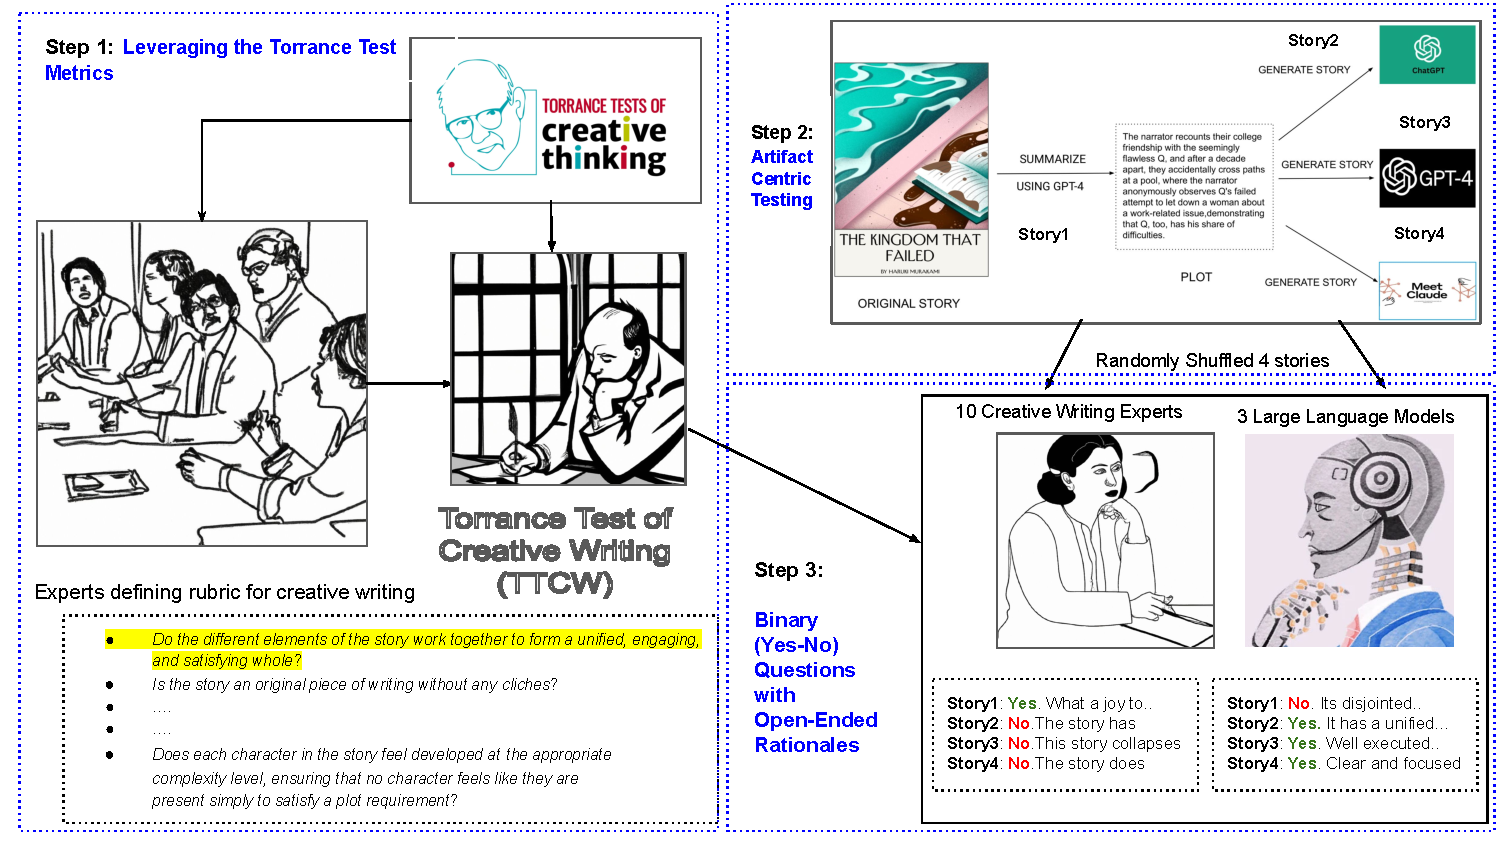
\includegraphics[width=\textwidth]{figures/CHI_pipeline.pdf}
\caption{\label{pipeline}Pipeline showing the construction of TTCW and evaluation of short stories using the TTCW framework where Step 1) shows how experts leverage the process-oriented Torrance Test of Creative Thinking to create 14 tests for evaluating creativity in short stories as a product. Step 2) demonstrates artifact-centric testing where 4 stories based on a single plot are used as a product of creativity evaluation Step3) shows an evaluation of stories using the TTCW framework by both expert humans and LLMs where they each provide Yes/No answers to individual tests followed by natural language rationales justifying their decision.}
\end{figure*}

To empirically validate TTCW as an evaluation protocol for creativity as product (fictional short stories), we build a benchmark consisting of 48 short stories: 12 stories written by professionals, and 36 by three top performing LLMs (ChatGPT \cite{ChatGPT}, GPT4 \cite{OpenAI2023GPT4TR} and Claude 1.3 \cite{Claude}) with 1400 words on average per story (Section~\ref{sec:data}; Figure \ref{pipeline} Step 2). %SM-rr I added Step 2
We recruit a new set of 10 experts, again adhering to CAT, to administer the 14 tests of TTCW on each story, collecting 3 evaluations per story. In this \textit{TTCW implementation with experts as assessors} (Figure \ref{pipeline} Step 3) %SM-rr I added Step 3
we aim to answer three research questions: 
\begin{enumerate}[label=RQ\arabic*:,leftmargin=3em]
     \item \textit{Is the TTCW-based creative evaluation consistent and reproducible? In other words, is there agreement among expert annotators when they perform tests on the same stories?} Based on a total of 2,000+ expert-administered tests, our findings reveal that experts reach moderate agreement on average (Fleiss Kappa 0.41) across the 14 TTCW tests, and reach strong agreement when considering the aggregated tests (Pearson correlation $0.69$). This confirms the validity of TTCW for the evaluation of creativity in fictional short stories.\\
     
    \item \textit{Are the human-written stories more likely to pass individual TTCW than LLM-generated stories? If so, which tests demonstrate the most significant gaps?} The analysis of the conducted tests reveals that the 12 expert-written stories pass an average of 84.7\% of the tests, confirming that although an expert story must not pass all tests to be deemed creative, experienced writers typically produce artifacts that pass the majority of the tests. In comparison, LLM-generated stories pass many fewer tests on average, from 9\% for ChatGPT-generated stories, up to 30\% for Claude-generated stories. In other words, LLM-generated stories are three to ten times less likely to pass individual TTCW tests compared to expert-written stories, revealing a wide gap in the evaluated creativity of LLM-generated content.\\ 
    
    \item \textit{Which LLMs perform better in TTCW evaluation, and are there specializations observed, with some different LLMs performing better on different Torrance dimensions?} Besides the general gap, the granularity of the TTCW reveals that individual LLMs differ in abilities, with GPT4 more likely to pass tests associated with Originality, and Claude V1.3 more likely to pass tests in Fluency, Flexibility and Elaboration.
\end{enumerate}

Prior work \cite{ippolito2022creative} has argued that given the nature of LLMs where they regurgitate text seen during pre-training, they are often unable to directly generate a truly original and creative piece of writing (Also see Section \ref{expertvsai}). However, they might be utilized in providing feedback to authors during their writing process \cite{chakrabarty2023creativity}. Thus, we perform a study of \textit{TTCW implementation with LLMs as assessors} (Section ~\ref{sec:llmeval}; and Figure \ref{pipeline} Step 3) %SM-rr I added Step 3
to understand whether LLMs can be used to assess creative writing. 
We expanded each test into a detailed prompt, and measured whether LLM assessments correlate with collected expert judgments. Our analysis reveals that for the most part, LLMs are not capable of administering the TTCW tests, as the three LLMs we experiment with achieve correlations with experts that are close to zero.

In summary, our work makes the following contributions:
\begin{itemize}
    \item We adapt the Torrance Test for Creative Thinking (TTCT), a protocol for evaluating creativity as a process, and align it for the evaluation of creativity as a product particularly focusing on short stories. Using the Consensual Assessment Technique, we design 14 tests called the \textit{Torrance Test for Creative Writing (TTCW)} based on the four original Torrance dimensions of fluency, flexibility, originality, and elaboration,
    \item We experimentally validate the TTCW through an assessment of 48 stories involving 10 participants with expertise in creative writing, finding that they reach moderate agreement when administering individual tests, and strong agreement when evaluating all tests in aggregate.
    \item We study the abilities of LLMs to generate stories that pass/fail the TTCW tests and their ability to reliably assess the creativity of stories following the TTCW framework through correlation with human judgments. Our findings show that LLM-generated stories are three to ten times less likely to pass TTCW tests compared to expert-written stories, as well as the fact that current state-of-the-art LLMs are not yet capable of reproducing expert assessments when administering TTCW tests. To enable future research in this fast-evolving domain, we release the large-scale annotation of 2,000+ TTCW assessments, each accompanied with a natural language expert explanation. 
    \item Finally, we discuss how creative writing experts can distinguish between AI vs. human written stories and how future work can use our evaluation framework for building rich interactive writing support tools.
\end{itemize}

\section{Related Work}
\subsection{Creativity Evaluation}
In prior work, \citet{baer2014creativity} argued how divergent thinking remains the most frequently used indicator of creativity in both creativity research and educational practice, and divergent thinking theory has a strong hold on everyday conceptions of what it means to be creative. Along the same lines, \citet{kaufman2008essentials} further discusses and evaluates common creativity measures such as divergent thinking tests, consensual technique, peer/teacher assessment, and self-assessment. \citet{silvia2008assessing} examined the reliability and validity of different subjective scoring methods for divergent thinking tests and introduced a new Top 2 scoring method that involves participants selecting their most creative responses, and demonstrates that this method yields reliable scores with a small number of raters. \citet{plucker2010assessment} discuss key issues and methods in creativity assessment including reliability, validity, bias, and use of assessments. \citet{beaty2021automating} explored the use of automated scoring via semantic distance, using natural language processing in assessing the quality of ideas in creativity research, demonstrating its strong predictive abilities for human creativity and novelty ratings across various tasks, thus addressing the labor cost and subjectivity issues in traditional human-rating methods.Like many of the prior works our research centers around grounding creativity evaluation through divergent thinking. In particular, we rely on the Torrance Tests of Creative Thinking (TTCT) as a foundation for measuring creativity.
\subsection{Evaluating Creative Writing}
Rubrics are one of the major tools for assessing writing which incorporate a set of prominent characteristics relevant to a specific type of discourse \cite{weigle2002assessing}. \citet{vaezi2019development} developed a rubric for the evaluation of fiction writing fiction through nine elements, namely narrative voice, characterization, story, setting, mood and atmosphere, language and writing mechanics, dialogue, plot, and image. To ensure its validity, they further recruited a number of distinguished creative writing professors to review this assessment tool and comment on its appropriateness for measuring the intended construct. \citet{biggs1982psychological} proposed to evaluate creative writing through the lens of the structural complexity of the product by utilizing the SOLO (Structure of the Observed Learning Outcome) taxonomy which buckets creative writing into incoherent (prestructural), linear(unistructural), conventional (multistructural), integrated (relational) and metaphoric (extended abstract). In prior work \citet{rodriguez2008problem} argued that narrative theory is key in teaching and grading creative writing. They emphasized how breaking down narrative elements such as plot, discourse-time, character, setting, narration, and filter delineates the tools authors use to effectively write fiction. In the creativity evaluation space \citet{baer2009assessing,amabile1982social} proposed \textit{The Consensual Assessment Technique} as a method of assessing creative performance on a real-world task such as writing a poem or a story. Unlike tests from the Torrance Tests of Creative Thinking (TTCT), the CAT does not rely on any specific criteria or test scores. The method proposes that the most valid assessment of the creativity of an idea or creation in any field is the collective judgment of experts in that field. Unlike prior work, we aim to align the evaluation of creativity as a process to the evaluation of creativity as a product with feedback from experts building upon prior theoretical works such as the TTCT and the CAT. Unlike prior work from \citet{vaezi2019development} where the rubric was created by surveying existing literature our work involved experts for creating the rubric from scratch without biasing their opinion or thought-process. Finally our rubric was validated by 5X more experts and across 3X more stories compared to that of \citet{vaezi2019development}.
\subsection{Expert Evaluation of Language Model Generations}
A cogent argument posits that the engagement with artistic prose isn't confined solely to specialists, but non-experts also can be competent in assessing imaginative prowess. Inheriting from research standards for large-scale natural language processing tasks, the majority of studies assessing the quality of generations from LLMs evaluate model performance by collecting data from crowd workers \cite{10.1145/3424636.3426903,rashkin-etal-2020-plotmachines,goldfarb-tarrant-etal-2020-content,roemmele-gordon-2018-linguistic,10.1609/aaai.v33i01.33017378}. Nevertheless, it is critical to acknowledge that during narrative evaluation trials involving both teachers in English and participants from Amazon Mechanical Turk, the study by \citet{karpinska-etal-2021-perils} exhibited that AMT contributors, even when shortlisted via rigorous eligibility parameters (unlike teachers), struggle to discriminate between model generated text and human-crafted references. \citet{clark-etal-2021-thats} run a similar study assessing non-expert's ability to distinguish between human and machine-authored text (GPT2 and GPT3) in three domains (stories, news articles, and recipes) and find that, without training, evaluators distinguished between GPT3 and human-authored text at random chance level. \citet{mirowski2023cowriting} emphasized why crowd workers are not a good fit for evaluating AI-generated screenplays and instead engage 15 experts—theatre and film industry professionals—who have both experiences in using AI writing tools and who have worked in TV, film, or theatre in one of these capacities: writer, actor, director, or producer for evaluating LLM generated screenplays. Finally, a recent study by \citet{veselovsky2023artificial} highlighted the fact that approximately 33-46\% of crowd workers on such platforms currently utilize large language models (LLMs) to complete any assigned task. Taking account of the above factors, for our work on evaluating short stories, we recruit creative writing experts ranging from professors to literary agents as well as MFA Fiction candidates.
\section{Design Considerations}\label{design}

One of the main contributions of our work is the collection of 14 tests, referred to as the \textit{Torrance Test for Creative Writing (TTCW)}, to evaluate creativity in short fictional stories. These tests were formulated through collaboration with domain experts which we detail in Section \ref{sec:approach}, but in this Section, we first present the design principles that shaped the methodology and provide the desiderata for the tests, which are then empirically validated.

\paragraph{Design Principle 1: Leveraging the Torrance Test Metrics.} The 14 tests we propose are grounded in the Torrance Test for Creative Thinking (TTCT) \cite{torrance1966torrance}, which has been a cornerstone in the evaluation of creativity.TTCT provides measures to understand the creative process through tasks that encompass unusual uses of objects, scenarios, and out-of-the-box problems. TTCT is centered around evaluating four dimensions of creativity

\begin{itemize}
\item \textbf{Fluency.} The sheer volume of meaningful ideas produced in reaction to a given stimulus.
\item \textbf{Flexibility.} The diversity of categories within the responses. 
\item \textbf{Originality.} The uniqueness or novelty of answers.
\item \textbf{Elaboration.} The depth or granularity of details within the responses.
\end{itemize}

While the direct applications of TTCT might exhibit limitations in terms of applicability across diverse creative domains \cite{amabile1982social,baer2009assessing}, its fundamental dimensions have proven adaptable. Researchers have repurposed these dimensions effectively in diverse sectors like science education \cite{trisnayanti2019development}, content strategies in marketing \cite{mcintyre2003individual}, and even in human-computer interaction, particularly interface design \cite{10.1145/3313831.3376495}.In Section \ref{sec:approach}, we show how using creative writing experts we design domain-specific tests grounded in each TTCT dimension. Feedback from these specialists further underscores the pertinence of these dimensions in assessing creative writing.

\paragraph{Design Principle 2: Artifact-centric Testing.}\footnote{In the context of creative writing we will refer to the "product" as artifact}  A key consideration when designing tests to evaluate creativity is whether to center the evaluation on the \textit{cognitive process} that leads to creativity or whether to evaluate the final artifact, which is a byproduct of the process \cite{mayers2007re}.
Much prior work -- including the TTCT -- takes a design-centric approach, as it includes richer observation of the evaluated individual, which might not be captured in the final artifact. However, process-oriented evaluation is limited in several ways. First, process-oriented evaluation is inherently limited by the quality of the observation of the individual's process. For instance, internal thoughts of the individual and other unrecorded activities can bias and lower the quality of the evaluation. Second, prior work has argued that neatly separating a process from an artifact is challenging, as the two are ``tightly integrated'' \cite{mayers2007re}, with ``the creative process leaving traces within the artifact'' \cite{murray2012craft}. Finally, observing the process is not always possible, particularly when evaluating the creativity of a preexisting artifact (e.g., a short story written years ago), or evaluating black-box agents such as LLMs, whose process cannot be observed in an interpretable way. We, therefore, follow prior work \citet{vaezi2019development,rodriguez2008problem} and design our creative writing evaluation to be artifact-centric.

\paragraph{Design Principle 3: Binary (Yes-No) Questions with Open-Ended Rationales.} In accordance with findings from prior work \cite{doi:10.1177/001316447103100307} which showed that reliability and validity are independent of the number of scale points
used for Likert-type items, we stick to a binary scale. The evaluation within each Torrance dimension follows a similar procedure. Each dimension is associated with multiple binary questions, that represent individual tests. Each binary question is formulated as having a Yes/No answer such that an artifact receiving a ``Yes'' answer to a question corresponds to the artifact passing the test. Additionally, the Yes/No answer should be accompanied by a free-text rationale written by the evaluator which justifies the chosen binary label, with a length expectation of at least 1-3 sentences. For each test, the combination of a structured binary assessment and an open-ended rationale are complementary. The binary assessment can be used for quantitative assessment, such as measuring agreement amongst evaluators, or comparative evaluation of a story collection (such as the one we perform in Section ~\ref{ref:humanresult}), whereas the rationale can be used for qualitative assessment, such as understanding concrete reasons for the passing or failing of a test, such as the analysis we perform in Section \ref{sec:analysis} centering around the most common themes that lead to the passing or failing of a given test.
\paragraph{Design Principle 4: Additive Nature of Tests.} Each question is intended to be independent of other questions (i.e., no question is a prerequisite to another question), but the creative assessment of a given artifact requires completing all the TTCW. 
The final assessment of a given artifact is the number of tests passed by the artifact, with the general expectation that passing more tests is directly proportional to the creativity of the artifact. In other words, the passing or failing of any single test cannot be interpreted as a final assessment of the creativity of an artifact, but rather the number of tests passed can paint a more complete picture of the creativity of the artifact. Analysis in Section ~\ref{ref:humanresult} confirms that our experts achieve on average moderate agreement on individual tests, but strong agreement when considering all tests in aggregate, confirming empirically the additive nature of the tests. In Section \ref{sec:approach}, we conduct a formative study with experts to formulate the fourteen TTCW that satisfy our design principles, which we then use in Section ~\ref{ref:humanresult} to run a evaluation of short stories using TTCW with experts as assessors. 

\section{Formative Study: Formulating the Torrance Tests For Creative Writing} \label{sec:approach}
We restricted the involvement of participants in our formative study to only those possessing either a structured educational background in creative writing (for instance, a Master of Fine Arts in Creative Writing), traditionally published authors \footnote{We do not recruit self-published authors}, or lecturers/professors instructing Fiction Writing at the university level. We specifically chose this filtering criterion to restrict our selection pool to experts in the field thereby aligning with the \textit{Consensual Assessment Technique}. Our recruitment resulted in participants who have published novels with leading publishing houses, students enrolled in top MFA programs in the United States, University professors teaching Fiction Writing, and screenwriters from prime-time networks. Participants were recruited through \textit{UserInterviews}~\footnote{\url{https://www.userinterviews.com}}, a professional freelancing website, and were paid \$70 for taking part in the hour-long survey. Table \ref{surveyprof} shows the background of the recruited participants. Our recruited participants span across different age groups, gender and professional expertise.

The formative study was structured in three parts. Initially, over video conferencing, experts were briefed on the study's primary objective, which aimed at devising actionable metrics for assessing creative writing, emphasizing fiction. They were also introduced to the Torrance Tests and the four specific dimensions encompassed by it. In the subsequent phase, participants were emailed the URL to a web app where they were asked to input their measures in text. They were instructed to allocate a 20-minute window to articulate up to five distinct measures corresponding to each of the Torrance dimensions first. This task was conducted without a sample fiction to maintain abstraction. The final phase involved presenting the participants with a sample fiction piece \footnote{\url{https://www.newyorker.com/books/flash-fiction/the-mirror}} on the same web app for evaluation, retrieved from The New Yorker. Participants were encouraged to use this as a tangible example to refine and augment their initial measures, ensuring they were grounded and practical. As an outcome of our study, we received 126 measures from the participants across the four Torrance dimensions. \footnote{The research was conducted at an institution that does not have an IRB approval process in place, but an Ethical Practices team reviewed the work and study protocols. We did not collect or share any PII during data collection, and participants could choose not to complete the survey and still receive a payment.}

\begin{table}[!ht]
\centering
\small
\begin{tabular}{|l|l|l|l|}
\hline
ID & Profession  & Gender & Age                \\ \hline
W1 & Professor of Creative Writing & Female & 45 \\ \hline
W2 & Professor of Creative Writing & Female & 56 \\ \hline
W3 & Lecturer in Creative Writing & Male & 40  \\ \hline
W4 & MFA Fiction Student & Male & 35        \\ \hline
W5 & MFA Fiction Student & Male & 31      \\ \hline
W6 & MFA Fiction Student & Female & 48         \\ \hline
W7 & Young Adult Fiction Writer  & Non-Binary & 39                      \\ \hline
W8 & ScreenWriter & Non-Binary & 34                  \\ \hline
\end{tabular}
\vspace{2ex}
\caption{\label{surveyprof}Background of Participants recruited for collecting judgments about Creativity across the dimensions of Torrance Test}
\end{table}

\begin{table}[!ht]
\centering
\small
\begin{tabular}{|l|l|l|}
\hline
Dimension & Expert Measure & Participants                  \\ \hline
\multirow{7}{*}{Fluency} & Narrative Pacing & W4,W6,W7 \\ \cline{2-3}
&\begin{tabular}[c]{@{}l@{}}Understandability\\ \& Coherence\end{tabular}  & W3,W7 \\ \cline{2-3}
&\begin{tabular}[c]{@{}l@{}}Language Proficiency\\ \& Literary Devices\end{tabular}  & W4,W2  \\ \cline{2-3}
&Narrative Ending & W3           \\ \cline{2-3}
&Scene vs Summary & W2,W5,W8          \\ \hline
\multirow{3}{*}{Flexibility} &Structural Flexibility & W1,W3,W8           \\ \cline{2-3}
& Perspective \& Voice Flexibility & W3,W6                        \\ \cline{2-3}
& Emotional Flexibility & W3                  \\ \hline
\multirow{5}{*}{Originality} & Originality in Theme/Content & W3,W6                 \\ \cline{2-3}
&Originality in Thought & \begin{tabular}[c]{@{}l@{}}W1,W2,W3,\\W5,W7\end{tabular}                  \\ \cline{2-3}
&Originality in Form & W2,W3,W4                  \\ \hline
\multirow{5}{*}{Elaboration} & World Building \& Setting & W2,W6                  \\ \cline{2-3}
&Rhetorical Complexity & W3,W4                  \\ \cline{2-3}
&Character Development & \begin{tabular}[c]{@{}l@{}}W2,W3,W4\\W5,W7,W8\end{tabular}                  \\ \hline
\end{tabular}
\vspace{2ex}
\caption{\label{testsource}Tests proposed and mapped by experts for evaluating story writing across TTCW dimensions}
\end{table}

\subsection{From Measures to Actionable Tests}
The measures derived from the participants exhibited a considerable degree of semantic congruence. For example, W2 proposed one way to measure Originality in Creative Writing as \textit{``Shows an innovative use of form/structure.''} while W4 proposed a similar measure \textit{Formal or stylistic novelty}.
W6 proposed one way to measure Elaboration depending on whether \textit{``The story has developed 3D characters.''} while W3 proposed an exactly similar measure but phrased it as \textit{``Does the piece make a flat character complex?''}. To consolidate these measures and develop a framework of the underlying tests for measuring creativity, we use a general inductive approach for analyzing qualitative data \cite{thomas2006general}. Following this method, three authors independently read all of the measures and assigned each measure an initial potential low-level group. Then, through repeated discussion, we reduced category overlap and created shared low-level groups associated. Finally, these low-level groups were collected into high-level groups, and a name was proposed for each group that encapsulates a generalized representation of the measures within the group. During the later meetings, an American Novelist and Creative Writing Professor were present to give further insights into the data.

In total, the tagging process yielded 14 distinct groups, 5 in the Fluency dimension, and 3 in Flexibility, Originality, and Elaboration. Table~\ref{testsource} presents the name we assigned to each group and the study participants that proposed a measure tagged within this group. For every group, we had a list of expert-suggested questions speaking about the same artifact. To choose a representative measure for every group, we selected the most well-articulated measure (in terms of word count). If the measure was already suggested as a question, we keep it intact; otherwise, we used the GPT4 model to convert a measure to a Yes/No question. For example, \textit{Originality suggests that the piece isn’t cliche $\rightarrow$ Is the story an original piece of writing without any
cliches?}
Next, we list each TTCW and provide the necessary background to contextualize the test. It should be noted that our tests are additive in nature. Failing a particular test should not be interpreted as the fact that the story doesn’t present any creative elements. Instead, it should be considered, by counting the number of distinct tests passed by a given story to obtain a more calibrated understanding of the creativity in a given piece.

\subsection{The Torrance Test for Creative Writing} \label{CreativityTest}

\paragraph{\textbf{{Fluency}}}: Compared with both reading and speaking fluency, writing fluency has always been traditionally harder to define \cite{abdel2013we}. Our 5 measures across this dimension each look at individual aspects of creative writing. 

\subsubsection{\textbf{{\color{blue} Narrative Pacing (TTCW Fluency1)}: Does the manipulation of time in terms of compression or stretching feel appropriate and balanced?}}This measure refers to the manipulation of time in storytelling for dramatic effect. Essentially, it is about controlling the perceived speed and rhythm at which a story unfolds. A skilled writer can manipulate the relationship between these two to affect the pacing of the narrative, either speeding it up (compression) or slowing it down (stretching). This technique plays a crucial role in shaping the reader's experience and engagement with the story. To assess narrative pacing, W4 suggested looking  ``\textit{Compression/stretching of time (story time vs. real world time)}'' while W6 and W7 advised to ``\textit{control the speed at which a story unfolds
\footnote{\url{https://www.writingclasses.com/toolbox/articles/stretching-and-shrinking-time}}.}''

\subsubsection{\textbf{{\color{blue}Scene vs Exposition (TTCW Fluency2)}: Does the story display awareness and insight into the balance between scene and summary/exposition?}} A `Scene' is a moment in the story that is dramatized in real-time, often featuring character interaction, dialogue, and action, while `Exposition', on the other hand, involves summarizing events or providing information like character history, setting details, or prior events. The right balance between scene and summary/exposition can vary depending on the story, but in general, it's essential for maintaining a good pace, keeping the reader engaged, and delivering necessary information \citet{burroway2019writing} 
\footnote{\url{https://creativenonfiction.org/syllabus/scene-summary/}}.
W2 strongly felt that fluent writing needs to ``\textit{display awareness and insight into the balance between scene and summary/exposition in the story.}'' while W5 and W8 emphasized the need for ``\textit{Enough dialogue to compensate for backstory.}''

\subsubsection{\textbf{{\color{blue}Language Proficiency \& Literary Devices (TTCW Fluency3)}: Does the story make sophisticated use of idiom or metaphor or literary allusion?}} Eminent novelist Milan Kundera said ``\textit{Metaphors are not to be trifled with. A single metaphor can give birth to love.}''. Sophisticated use of literary allusion or figurative language such as metaphor/idioms often add depth, interest, and nuanced meaning to any creative writing. It allows for a richer reading experience, where the literal events are imbued with deeper symbolic or thematic significance. W4 and W2 both emphasized the presence of ``\textit{Sophisticated use of idiom, metaphor, and literary allusion} or \textit{Surprising, skilled, and complex use of metaphor/simile/allusion} as a way to measure Fluency in creative writing.
\subsubsection{\textbf{{\color{blue}Narrative Ending (TTCW Fluency4)}: Does the end of the story feel natural and earned, as opposed to
arbitrary or abrupt?}} In her New Yorker essay ``On Bad Endings'' \cite{BadEndings} Accocela writes ``Another possibility is that the author just gets tired. I review a lot of books, many of them non-fiction. Again and again, the last chapters are hasty and dull. `I’ve worked hard enough,' the author seems to be saying. `My advance wasn’t much. I already have an idea for my next book. Get me out of here'.''
If the writer ends the piece simply because they are ``tired of writing'', the conclusion might feel abrupt, disjointed, or unfulfilling to the reader. This is one of the important factors of creative writing fluency. A strong ending offers a sense of closure, ties up the central conflicts or questions of the story, and generally leaves the reader feeling that the narrative journey was worthwhile and complete. For this measure of Fluency, W3 asked  ``\textit{Does the writer know how to end the piece not because they're tired of writing, but because they have come to the moment the entire piece has been leading us towards?}''
\subsubsection{\textbf{{\color{blue}Understandability \& Coherence (TTCW Fluency5)}: Do the different elements of the story work together to form a unified, engaging, and satisfying whole?}} Narrative coherence is the degree to which a story makes sense  \footnote{https://en.wikipedia.org/wiki/Narrative\_paradigm}. A well-crafted story usually follows a logical path, where the events in the beginning set up the middle, which then logically leads to the end. Every scene, character action, and piece of dialogue should serve the story and propel it forward. Well-written stories have an underlying unity that binds the elements together. W3 strongly advocated for this measure by saying ``\textit{Does the piece hold together? In other words, does the beginning lead through the middle to the end in a way that feels deliberate and intentional? This is the difference between several pages of writing and a PIECE of writing. Great writing errs on the side of unity over disorder.}'' while W7 suggested the importance of this measure through ``\textit{a logical flow.''}

\paragraph{\textbf{Flexibility}} Flexibility is often referred to as the ability to look at something from a different angle or point of view. In the context of creative writing, our participants agreed on 3 distinct measures of Flexibility.
\subsubsection{\textbf{{\color{blue}Perspective \& Voice Flexibility (TTCW Flexibility1)}: Does the story provide diverse perspectives, and if there are unlikeable characters, are their perspectives presented convincingly and accurately?}} An \textit{omniscient} narrator is the all-knowing voice in a story that can convincingly and accurately depict a wide range of character viewpoints, including those of characters who may be morally ambiguous, difficult, or otherwise unappealing. As stated in \citet{friedman1955point} an omniscient narrator enhances a sense of reliability or truth within literary works since readers are given deeper insights into many characters. The multiple viewpoints feel more objective because readers have access to multiple interpretations of events and can thus decide how they feel about each character’s perspective. W3 wanted ``\textit{a writer to be able to inhabit various perspectives, even unlikable ones.}'' while W6 suggested ``\textit{Flexibility of voice. Can the author inhabit the consciousness of different characters and not just likable ones?}"
\subsubsection{\textbf{{\color{blue}Emotional Flexibility (TTCW Flexibility2)} : Does the story achieve a good balance between interiority and exteriority, in a way that feels emotionally flexible?}}
Emotional flexibility is asking whether the piece of writing effectively balances action and introspection, and if it portrays a broad and realistic spectrum of emotions as corroborated by W3. \textit{Exteriority} refers to the observable actions, behaviors, or dialogue of a character, and the physical or visible aspects of the setting, plot, and conflicts.\textit{Interiority}, on the other hand, pertains to the inner life of a character — their thoughts, feelings, memories, and subjective experiences. A balance between these two aspects is crucial in creating well-rounded characters and compelling narratives. As stated in \citet{campe2014rethinking} if a story is too heavy on exteriority, it may feel shallow or lack emotional depth. If it leans too much on interiority, it could become overly introspective and potentially lose the momentum of the plot.
\subsubsection{\textbf{{\color{blue} Structural Flexibility(TTCW Flexibility3)}: Does the story contain turns that are both surprising and appropriate?}} A good piece of creative writing often has plot twists, character developments, or thematic revelations that surprise the reader, subverting their expectations in a thrilling way. However, despite the surprises and twists, the turns in the story must also make sense within the established context of the story's universe, its characters, and its themes. It shouldn't feel like the writer has broken the rules they've set up, or made a character behave inconsistently without reason, simply for the sake of shock value. In order for any writing to be structurally flexible W3 wanted to ensure that ``\textit{the writer capable of making turns in the work that are both surprising and appropriate} while W1 required the presence of ``\textit{New twist in the story that are believable} to measure structural flexibility
\paragraph{\textbf{{Originality}}} Creative writing requires originality, or the ability to generate unique ideas \cite{ward1999creative}.
Our participants suggested three unique ways in which they look for originality in creative writing.

\subsubsection{\textbf{{\color{blue}Originality in Theme and Content (TTCW Originality1)}: Will an average reader of this story obtain a unique and original idea from reading it?}} In his book ``Literature and the Brain'' well-known literary critic and scholar Norman Holland discusses how stories stimulate the mind and impact readers \citet{holland2009literature}. A good story that offers a deeper understanding of human nature, cultural insights, unique viewpoints, or even the exploration of new ideas and themes has a lasting impact on its reader and society. In ``Poetic Justice'', prominent philosophers Martha Nussbaum explores how the literary imagination is an essential ingredient of public discourse and a democratic society \citet{nussbaum1997poetic}. As such originality in theme and content is an important measure of creative writing. In the words of W6 originality in theme meant  ``\textit{New brilliant ideas about the future and humanity (mostly in speculative fiction). Does the writing have an original message?} while W3 mentioned ``\textit{Do I feel I am learning something new from the piece? What is the purpose of putting it into the world?}''
\subsubsection{\textbf{{\color{blue} Originality in Thought (TTCW Originality2)}: Is the story an original piece of writing without any cliches?}} A cliche is an idea, expression, character, or plot that has been overused to the point of losing its original meaning or impact \citet{fountain2012cliches}. They often become predictable and uninteresting for the reader. In his book \citet{clark2008writing} eminent American writer, editor, and writing coach: Roy Peter Clark advised writers to strictly avoid cliches because they often indicate a lack of original thought or laziness in language use. Originality suggests that the piece isn't cliche. Several experts agreed on this measure with W3 saying ``\textit{Originality suggests that the piece isn't cliche.} while W4 required ``\textit{Plot that is surprising rather than cliche}''. W6 emphasized originality in thought through ``\textit{writing that is not cliche, not recycled tropes, and does not contain stereotyped one-dimensional characters}
\subsubsection{\textbf{{\color{blue}TTCW Originality in Form \& Structure (Originality3)} : Does the story show originality in its form?}} In his book \citet{boardman1992narrative} Frederic Jameson highlighted the complexities of postmodern literature, where the blurring of genres and innovation in form was a key characteristic \citet{jameson1991postmodernism}. Originality in form has also been accomplished by the unconventional use of format, genre, or narrative structure or arc. For instance, the Pulitzer-winning book \textit{The Color Purple} by Alice Walker is told through a series of letters written by the protagonist. Neil Gaiman's \textit{American Gods} on the other hand combines elements of fantasy, mystery, and mythic fiction in unexpected ways. \textit{The Sound and the Fury} by William Faulkner deviates from the traditional plot structure by presenting a narrative that unfolds through the stream of consciousness of different characters. The goal of originality in form or structure is often to provide a fresh reader experience, challenge conventional reading expectations, or to create a deeper or more complex exploration of the story's themes. This was corroborated by W2 and W5 who wanted to see ``\textit{formal or stylistic novelty}. W3 also wanted to see if \textit{A piece demonstrates original ways to work in sometimes tired forms (such as the short story)}
\paragraph{\textbf{{{Elaboration}}}}
Elaboration in creative writing is the process of adding details and information to a story to make it more interesting and engaging. This can be done by describing the setting, characters, and action in more detail, or by adding dialogue, thoughts, and feelings to the story.

\subsubsection{\textbf{{\color{blue} World Building and Setting (TTCW Elaboration1)}: Does the writer make the fictional world believable at the sensory level?}} American poet and memoirist Mark Doty discuss the importance of creating a vivid, immersive reality at the sensory level through the use of detailed, evocative description \cite{doty2014art}. An effective writer often uses sensory details to paint a detailed picture of the story's environment, making it feel tangible and real to the reader. This level of detail contributes to the believability of the world, even if it is a completely fictional or fantastical setting. It helps the reader to suspend disbelief and become more deeply invested in the narrative. W2 suggested measuring elaboration through ``\textit{Use of setting to inform the action and atmosphere of the story without succumbing to pathetic fallacy}''. W6 further confirmed the same by saying ``\textit{There is a setting. The short story is rooted in a time and a place. If it's science fiction or fantasy there will be some world building.}''. W5 further mentioned ``\textit{the presence of a self-consistent world}'' as a measure of elaboration while W3 asked ``\textit{How does the writer make the fictional world believable at the sensory level?}
\subsubsection{\textbf{{\color{blue}Character Development (TTCW Elaboration2)}: Does each character in the story feel developed at the appropriate complexity level, ensuring that no character feels like they are present simply to satisfy a plot requirement?}} A 'flat character' is typically a minor character who is not thoroughly developed or who does not undergo significant change or growth throughout the story. They often embody or represent a single trait or idea, and they're only used to advance the plot or highlight certain qualities in other characters. A 'complex character' on the other hand also known as a round character, has depth in feelings and passions, has a variety of traits of a real human being, and evolves over time. \citet{forster1927aspects,fishelov1990types,currie1990nature} highlights that any creative piece of fiction or non-fiction tends to be more engaging to the reader when authors can take a character who initially appears to be one-dimensional or stereotypical (flat) and add depth to them, as it mirrors the complexity of real people. Multiple experts emphasized on the importance of character development. For instance, W6 thought ``\textit{The story should have developed 3D characters.} while W2 and W8 asked for ``\textit{Complex character development that avoids stereotype, generalization, trope, etc}''. W3 wanted to see ``\textit{Does the piece make a flat character complex?}
\subsubsection{\textbf{{\color{blue}Rhetorical Complexity (TTCW Elaboration3)}: Does the story operate at multiple ``levels'' of meaning (surface and subtext)?}}In Ernest Hemingway's short story ``Hills Like White Elephants,'' the couple's conversation about seemingly unrelated topics implies a much deeper and more serious discussion about abortion. Their actual dialogue never directly addresses this issue, but it's heavily suggested through what's left unsaid — the subtext. Effective writing often operates on both surface and subtext levels. The surface text keeps the reader engaged with the plot and characters, while the subtext provides depth, complexity, and additional layers of interpretation, contributing to a richer and more rewarding reading experience \citet{kochis2007baxter,phelan1996narrative}. W3 asked for rhetorical complexity by saying ``\textit{Is there a sense of the piece being complex in such a way that it needed to be written as a whole, not simply paraphrased or summed up?} while W4 mentioned that ``\textit{Text should operate at multiple levels of meaning (surface and subtext)}.''

\section{TTCW Implementation with Experts as Assessors} \label{sec:data}
In this Section, we detail our implementation of creative writing evaluation using the TTCW framework derived previously. We first carefully select the 48 short stories included in the evaluation, then go over the 2.5-hour study design protocol that our 10 experiment participants followed, and finally analyze the results based on the 2,000+ individual tests administered by the experts. We leverage the collected annotations to answer the following research questions:
\begin{enumerate}[label=RQ\arabic*:,leftmargin=2.5em]
    \item \textit{Are the human-written New Yorker stories more likely to pass individual TTCW than LLM-generated stories? If so, which tests demonstrate the most significant gaps?}
    \item \textit{Is the TTCW-based creative evaluation consistent and reproducible? In other words, is there agreement among expert annotators when they perform tests for similar stories?}
    \item \textit{Which LLMs perform better in TTCW evaluation, and are there specializations observed, with some different LLMs performing better on different Torrance dimensions?}
\end{enumerate}

\subsection{Data Selection}

\begin{figure*}
\centering
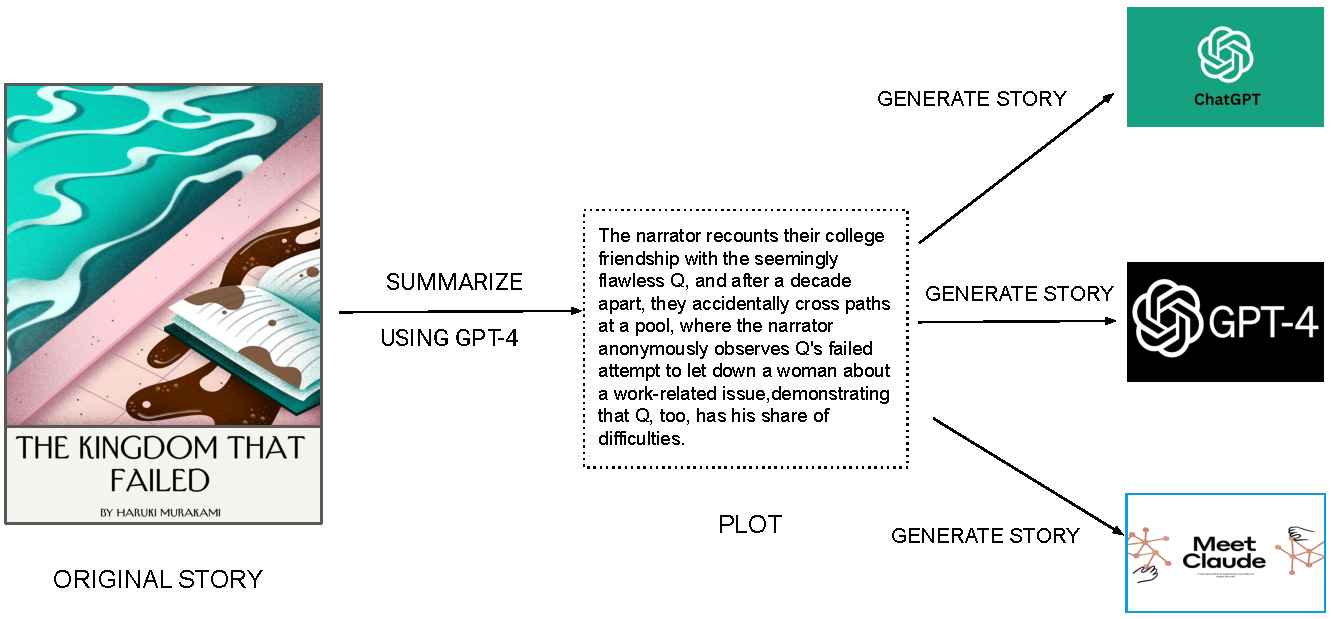
\includegraphics[width=\textwidth]{figures/datapipeline.pdf}
\caption{\label{datapipeline}Pipeline showing how our test set is created for evaluation. For each human-written original New Yorker story, we generate 3 stories from one LLM each, based on the plot of the original story. The plot is a single-sentence summary of the original story automatically generated by GPT-4 and verified by humans.}
\end{figure*}

Prior studies in the creativity of model-generated text have shown that technologies such as LLMs are capable of generative long and coherent stories \cite{yang2022doc,yang2022re3}, as well as act as assist and collaborate with creative writers \cite{yuan2022wordcraft,ippolito2022creative,mirowski2023cowriting}. For practical considerations, these studies limit their evaluation solely to model-generated content, typically only claiming relative improvements from one system to another, and do not establish whether a gap remains between high-quality human-written stories and model-generated text. Our research employs a rigorous evaluation protocol that juxtaposes human-written short stories against those constructed by LLMs to discern the potential gap, if any, in their creative quality. The dataset selection process is visually summarized in Figure~\ref{datapipeline}. We first collect 12 short stories from The New Yorker collection of short stories \footnote{https://www.newyorker.com/tag/short-stories}. Our selection criterion involved choosing short stories with diverse authors and plots. Spanning from August 13, 2020, to May 8, 2023, these stories (ranging between 1000 to 2,400 words as delineated in Figure \ref{lengthdist} in the Appendix) include compositions from acclaimed authors such as Haruki Murakami to Nobel laureate Annie Ernaux. The titles and a one-sentence plot summary (generated by GPT-4 and verified by humans) of included New Yorker short stories are listed in Table ~\ref{teststories} in Appendix.

We prompt three top-performing LLMs: GPT3.5, GPT4, and Claude V1.3 to generate a story of similar length to each New Yorker story, based on the one-sentence plot summary. We note that the choice to condition model-generated stories on the plot of the New Yorker story is an important design consideration of our evaluation. First, LLMs are known to have limited ability in devising original plotlines, as highlighted in previous research \cite{ippolito2022creative}. Second, it creates groups of stories that center around a common plot, allowing to dissociating evaluation of a story's form (i.e., creative writing), from the evaluation of plot-line creativity. 

Although LLMs were prompted to generate stories of a given length, initial experimentation by the authors of the paper revealed that the LLMs typically generate stories that can be 20-50\% more concise than intended. Length is a known confounding factor in text generation evaluation, for example with work showing that evaluators systematically prefer longer summaries as they tend to be more informative \cite{stiennon2020learning}. To address this limitation, we employed an iterative mechanism that prompted the LLM to iteratively expand on its initial story until the divergence in word count between the AI-generated and its paired human-written story was less than 200 ( See Prompt in Table \ref{promptstory} in Appendix). In our processing, all LLMs were able to converge to the desired length in at most 20 iterations. The procedure yields a total of 12 story groups, each consisting of one New Yorker story, and three LLM-generated stories, all following a common plot-line and having very similar length, for a total of 48 short stories.
We also experimented with a few other choices in prompt design such as adding \textit{You are an expert of creative fiction writing} to the beginning of the prompt or demonstrating an example New Yorker story in the prompt but these did not lead to any appreciable difference in the quality of the stories based on preliminary evaluation.

In our experiments, the stories either originate from experts or LLMs, and we do not include stories written by non-experts or `amateurs'. Although this was a consideration in the initial phases of the project, collecting amateur-written stories turned out to be a challenging and expensive process. Given the way our experiments are designed, it would require recruiting 12 non-experts to write stories given a plot since each expert-written story comes from a distinct author. The definition of an `expert' or `amateur' creative writer is difficult in a field that has unclear professional delineations. Collecting expert-written stories is straightforward as we rely on publication venue as a signal but identifying amateur writers is in itself a challenging task and might entail certain selection biases. A story written by any individual otherwise deemed as `amateur' can still be of considerable high quality. Another alternative we considered is resorting to crowd-working platforms to recruit amateurs for writing stories but a recent study by \citet{veselovsky2023artificial} highlighted the fact that approximately 33-46\% of crowd workers on such platforms currently utilize large language models (LLMs) to complete any assigned task, which would negatively impact our experiments' reproducibility. Finally adding amateur-written stories would require increased budgets for evaluation. These difficulties govern our decision not to include amateur-written stories.
\subsection{Evaluation Protocol}

\subsubsection{Expanded Expert Measure and Prompt Design} \label{sec:prompting}

\begin{table*}[!ht]
\centering
\small
\begin{tabular}{|l|l|}
\hline
\begin{tabular}[c]{@{}l@{}}Expert \\ Measure\end{tabular}               & Does the writer make the fictional world believable at the sensory level?                                                                                                                                     \\ \hline
\begin{tabular}[c]{@{}l@{}}Expanded\\ Expert\\ Measure (M)\end{tabular} & \begin{tabular}[c]{@{}l@{}}Sensory details pertain to the five senses - sight, sound, touch, taste, and smell. An effective \\ writer can use these elements to paint a detailed picture of the story's environment, making\\ it feel tangible and real to the reader.\\ \\ For example, describing the specific colors and shapes in a scene, the sounds that fill a space,the \\ textures and temperatures that a character comes into contact with, the flavors of the food they \\ eat, or the scents that fill the air, can all contribute to creating a sensory-rich and believable world.\\ \\ By stimulating the reader's senses, the writer can make the reader feel as though they're \\ experiencing the events of the story firsthand.This level of detail contributes to the believability of\\ the world, even if it's a completely fictional or fantastical setting. It helps the reader to suspend\\ disbelief and become more deeply invested in the narrative.\end{tabular} \\ \hline
\begin{tabular}[c]{@{}l@{}}Human\\ Instruction\end{tabular}             & \begin{tabular}[c]{@{}l@{}}\{\{M\}\}\\ \\ Based on the story that you just read, answer the following question.\\ \textit{\color{blue}Does the writer make the fictional world believable at the sensory level?}\\ -Yes \\ -No \\\\ Reasoning : \end{tabular}                                                                       \\ \hline
\begin{tabular}[c]{@{}l@{}}LLM\\ Instruction\end{tabular}               & \begin{tabular}[c]{@{}l@{}}\{\{M\}\}\\ \\ Given the story above, list out the elements in the story that call to each of the\\ five senses. Then overall, give your reasoning about the question below and give\\ an answer to it between 'Yes' or 'No' only\\ \\ \textit{\color{blue} Q) Does the writer make the fictional world believable at the sensory level?}\end{tabular}                                                                                                                                                                                                                                 \\ \hline
\end{tabular}
\vspace{2ex}
\caption{\label{prompting1}Expert suggested question for World Building and setting (Row1) ; Expanded Expert Measure (Row2); Elucidated prompt designed for other expert humans
(Row3); Elucidated quantifiable prompt designed for Large Language Models that elicit Chain of Thought Reasoning(Row4) }
\vspace{-5ex}
\end{table*}

We want these tests described above to be understandable by both other creative writing experts or even LLMs, such that they can be used for evaluation purposes. An expert suggested questions for empirically evaluating creative writing might frequently elicit ambiguity in Large Language Models or even other creative writing experts. In order for LLMs or other experts to comprehend the suggested questions in Section
\ref{CreativityTest}, we attempt to expand them by adding more details.
Recent pre-trained LLMs (e.g., GPT-4 \cite{OpenAI2023GPT4TR} GPT3.5 \cite{ChatGPT}) can engage in fluent, multi-turn conversations out of the box, substantially lowering the data and programming-skill barriers to creating passable conversational user experiences. People can improve LLM outputs by prepending prompts—textual instructions and examples of their desired interactions—to LLM inputs. The prompts steer the model towards generating the desired outputs, raising the ceiling of what conversational UX is achievable for non-AI experts. To elucidate these questions we prompt GPT4 with the following instruction: \textit{What do creative experts mean when they say the following: \{\{expert question\}\}}. Once GPT4 gives a response 3 domain experts carefully verify the response and edit it where required. Table \ref{prompting1} (Row2) 
shows the human-verified GPT4 expanded expert measure in response to the input prompt. Table \ref{prompting1} (Row3; Human Instruction) shows the final instruction given to human experts during the evaluation of our stories that contains the expanded expert measure \{\{M\}\} in addition to the original yes/no question.More examples of Human Instructions for the remaining 13 tests are provided in Section \ref{allprompts} in the Appendix.

\begin{table}[!ht]
\centering
\small
\begin{tabular}{|l|l|l|l|}
\hline
ID & Profession  & Gender & Age                \\ \hline
E1 & Lecturer of Creative Writing & Male & 42 \\ \hline
E2 & Lecturer of Creative Writing & Male & 32 \\ \hline
E3 & Professor of Creative Writing & Male & 46  \\ \hline
E4 & Professor of Creative Writing & Female & 43 \\ \hline
E5 & Literary Agent & Male & 29 \\ \hline
E6 & Literary Agent & Female & 30  \\ \hline
E7 & Writer with an MFA in Fiction & Non-Binary &  25       \\ \hline
E8 & Writer with an MFA in Fiction & Male & 24      \\ \hline
E9 & Writer with an MFA in Fiction & Male & 28      \\ \hline
E10 & Writer with an MFA in Poetry  & Male & 30                      \\ \hline
\end{tabular}
\vspace{2ex}
\caption{\label{creativeexperts}Background of creative writing experts recruited for evaluating the stories from our test set}
\vspace{-3ex}
\end{table}

\begin{table*}[!ht]
\small
\centering
\begin{tabular}{|l|l|l|l|l|l|l|}
\hline
Dimension & Test & GPT3.5 & GPT4 & Claudev1.3 & NewYorker & Expert Agreement \\ \hline
\multirow{5}{*}{Fluency} & Understandability \& Coherence & 22.2 & 33.3 & 55.6 & \textbf{91.7} & 0.27 \\ \cline{2-7}
& Narrative Pacing & 8.3 & 52.8 & 61.1 & \textbf{94.4} & 0.39 \\ \cline{2-7}
& Scene vs Exposition & 8.3 & 50.0 & 58.3 & \textbf{91.7} & 0.27 \\ \cline{2-7}
& Literary Devices \& Language Proficiency & 5.6 & 36.1 & 13.9 & \textbf{88.9} & 0.37 \\ \cline{2-7}
& Narrative Ending & 8.3 & 19.4 & 33.3 & \textbf{91.7} & 0.48 \\ \hline\hline
\multirow{3}{*}{Flexibility} & Emotional Flexibility & 16.7 & 19.4 & 36.1 & \textbf{91.7} & 0.32 \\ \cline{2-7}
& Perspective \& Voice Flexibility & 8.3 & 16.7 & 19.4 & \textbf{72.2} & 0.44 \\ \cline{2-7}
& Structural Flexibility & 11.1 & 19.4 & 30.6 & \textbf{88.9} & 0.39 \\ \hline\hline
\multirow{3}{*}{Originality} & Originality in Form & 2.8 & 8.3 & 0.0 & \textbf{63.9} & 0.41 \\ \cline{2-7}
& Originality in Thought & 2.8 & 44.4 & 19.4 & \textbf{91.7} & 0.40 \\ \cline{2-7}
& Originality in Theme \& Content & 0 & 19.4 & 11.1 & \textbf{75.0} & 0.66 \\ \hline\hline
\multirow{3}{*}{Elaboration} & World Building \& Setting & 16.7 & 41.7 & 58.3 & \textbf{94.4} & 0.33 \\ \cline{2-7}
& Character Development & 8.3 & 16.7 & 16.7 & \textbf{61.1} & 0.31 \\ \cline{2-7}
& Rhetorical Complexity & 2.8 & 11.1 & 5.6 & \textbf{88.9} & 0.66 \\ \hline\hline
\multicolumn{2}{|c|}{Average} & 8.7 &27.9 & 30.0 & \textbf{84.7} & 0.41 \\ \hline
\end{tabular}
\vspace{2ex}
\caption{\label{absolutehumaneval} Average passing rate on individual TTCW, based on annotations of 10 creative writing experts across the 48 stories in our collection, authored by GPT3.5, GPT4, Claude, and expert human writers published in the New Yorker along with agreement measures (Fleiss Kappa) on individual test.}
\end{table*}

\subsubsection{Expert Evaluation Protocol}
\label{experteval}
We developed an evaluation protocol tailored specifically for experts in the domain of creative writing. The protocol, designed to be completed in approximately 2 to 2.5 hours, centered around a rigorous assessment of tuples of four distinct stories (one New Yorker story and the associated LLM-generated stories by the three LLMs) using the TTCW. The study was structured as follows:

\begin{enumerate}
    \item The four stories in a group were shuffled, and anonymized (i.e., the author of the story was not visible to the evaluator).
    \item The expert evaluator read the first story in its entirety and then administered the fourteen TTCW tests by assigning a Yes/No label and providing a justification for the label.
    \item Upon completing the evaluation of the first story in the group, the evaluator proceeded to read and evaluate the second, third, and fourth stories in the group respectively. The evaluators were also allowed to edit their responses at any point of time during the entire process.
    \item Once the evaluator had completed the TTCW evaluation of the four stories within a group, they were asked to rank all four stories in terms of subjective preference, and were asked to make an estimated guess of each story's origin: choosing from ``An experienced writer'', ``An amateur writer'', or ``Written by AI.'' The exact formulation of each question is given in Figure~\ref{relev} in the Appendix.
\end{enumerate}

In preliminary trials conducted by the authors of the paper, the entire task completion was observed to range from 2-2.5 hours. Consequently, an \$80 remuneration was determined to appropriately acknowledge the expertise of participants and encourage them to provide detailed justifications in their TTCW assessments. We note that participants were not provided details on the process used to create the groups of four stories, and were not told that each group consisted of one human-written story and 3 LLM-generated stories. Participants were explicitly instructed to avoid using search engines, which might reveal the origin of the New Yorker story. We also ensured beforehand that the participants were not familiar with any of the stories within a given group. Finally, participants were permitted to take breaks during the study but were encouraged to complete the entire task within a 24-hour window, so they would clearly remember each story when completing the final comparative task.

\subsection{Participant Recruitment}
\label{participant}

To test the robustness and validity of TTCW-based evaluation, we chose to recruit a new set of experts to conduct the evaluation and not re-hire the ones from our formative study that played a role in the creation of the tests. We posit that such a choice demonstrates the fact that the TTCW can be administered by any expert provided solely with the tests and their expanded explanations. We recruited 10 participants on the \textit{User Interviews} platform and listed their background in Table~\ref{creativeexperts}. Four of these participants are associated with the creative writing departments at leading American academic institutions, with considerable experience conducting undergraduate and graduate-level courses. Two participants function as literary agents at a top-tier, full-service US literary agency representing well-recognized authors, and four are professional writers with a Master of Fine Arts in Fiction or Poetry.

To experimentally analyze the reproducibility and validity of the TTCW, we randomly assigned each story group to 3 distinct experts. This allows us to study the agreement levels between experts on individual tests as well as in aggregate. After each task, an expert participant was given the option to receive another group of stories, and our participants completed on average 3.6 tasks over 3 weeks, for a total of 36 assessments (i.e., 3 for each of the twelve groups). Because each assessment contains four stories, and each story was evaluated using the 14 TTCW, we collected a total of 2,016 binary labels and expert-written justifications for these labels.
\subsection{Results} \label{ref:humanresult}
\subsubsection{Analyzing Pass Rates of Stories}
\begin{figure*}
    \centering
    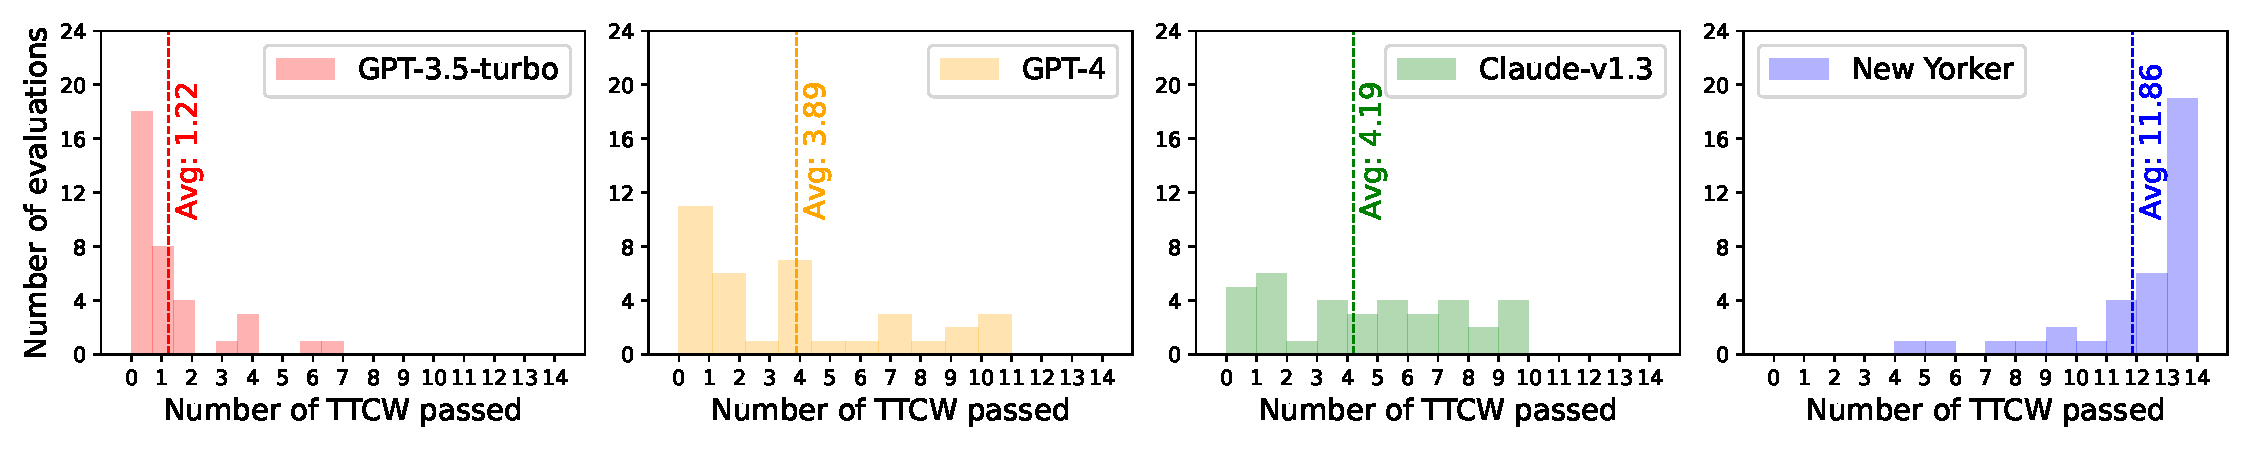
\includegraphics[width=0.95\textwidth]{figures/Creativity_Aggregate_Performance.pdf}
    \caption{Distribution of aggregate TTCW results, in which only the number of tests passed is retained. }
    \label{fig:ttcw_aggregate_histogram}
\end{figure*}

\begin{figure*}[!ht]
    \subfloat[Likert plot showing ranking of stories within an individual group based on all expert preferences]{\frame{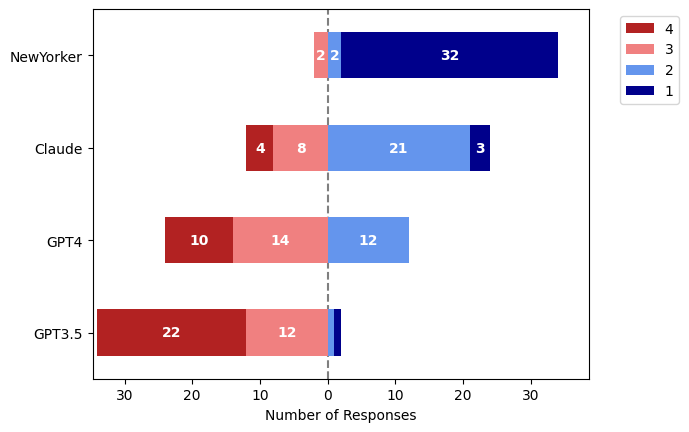
\includegraphics[width=0.44\textwidth]{figures/relativerank.png}}} \quad
    \subfloat[Likert plot showing how often authors attributed the source of the stories correctly]{\frame{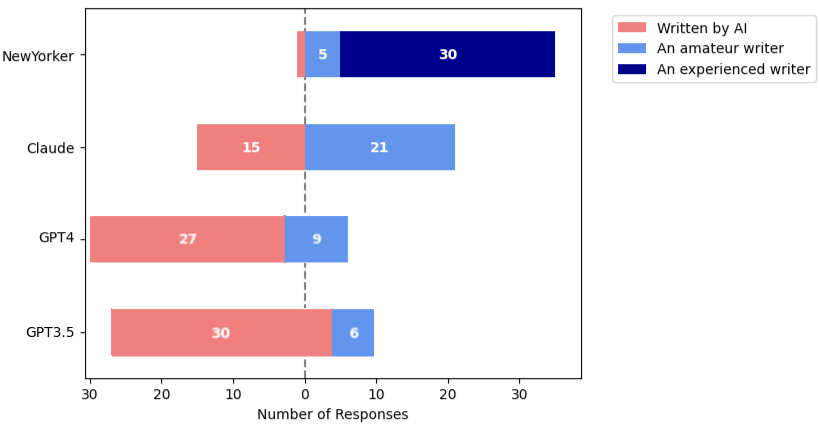
\includegraphics[width=0.53\textwidth]{figures/relativeauthor.png}}} 
    \caption{\label{relativehumaneval1} \textbf{Relative Evaluation} Left figure showing ranking preference assigned to each story within a group. Right figure showing how creative experts attributed any given story from The NewYorker or 3 LLMs to one of the options between An experienced writer, An amateur writer, or An AI }
\end{figure*}

Table ~\ref{absolutehumaneval} summarizes the average \textit{passing rate} on the 14 TTCW for each of the four story types (GPT3.5, GPT4, Claude-v1.3, and New Yorker). Passing rate here corresponds to the percentage of time expert participants answer `Yes' to an individual TTCW for any given story. The New Yorker stories widely achieve the highest passing rate on all fourteen tests, with an overall pass rate of 84.7\%. In other words, individual New Yorker stories are assessed to pass 11.9 of the 14 TTCW on average. When examining performance on individual tests, no test receives a pass rate of 100\%, confirming that no test is an absolute requirement in high-quality creative writing, and experimentally justifying the need to conduct the TTCW tests as a set (Design Principle 4).

Moving to the performance of the LLM-generated stories, passing rates are much lower, with GPT3.5 stories passing less than 10\% of TTCW, while GPT4 and Claude v1.3 are closer to 30.0\%. In other words, LLM-generated stories pass between a third and a tenth of the TTCW compared to human-written New Yorker stories. When breaking down LLM-story performance across the Torrance dimensions, all models achieve their highest pass rate on the Fluency dimension, and Claude v1.3 achieves the highest performance on average across Fluency, Flexibility, and Elaboration, while GPT4 scores highest on the Originality dimension. This experimental finding is surprising as Claude v1.3 is an LLM that is smaller in size(52B) than GPT4 \footnote{https://the-decoder.com/gpt-4-architecture-datasets-costs-and-more-leaked/}. 

\subsubsection{Reproducibility of TTCW}

Since we collected three independent TTCW evaluations for each story, we can report the agreement levels of experts when they conduct the tests individually, and their assessment in aggregate. We compute the Fleiss $\kappa$ agreement across all annotations and report the interrater agreement level of each test in Table ~\ref{absolutehumaneval}. Individual test agreement ranges from 0.27 to 0.66, and averages at 0.41, suggesting moderate agreement on most of the individual TTCW.

Since the TTCW are designed to be additive, we further compute an aggregate score for each story by counting the number of TTCW tests a story passes. We visualize the results of this aggregate measure in Figure ~\ref{fig:ttcw_aggregate_histogram}. Since the aggregate measure is numerical (ranges from 0 to 14), we use Pearson correlation to measure agreement among experts. At this aggregate level, we obtain a correlation($\rho$) of 0.69, showing strong agreement among experts on the number of tests a story passes. In other words, even though experts reach slightly lower agreement on which exact TTCW a story passes or fails, they achieve strong agreement on the number of tests a story passes overall. This experimental finding confirms the importance of Design Principle 4, and the need for the tests to be performed as a set to achieve a reproducible evaluation of creativity for a given short story. When the objective is to evaluate the broad creativity in a short story, we recommend that all fourteen tests be administered as a set by one expert annotator, rather than by different experts or administering only an individual test, as this increases the reproducibility of the results.
\subsubsection{Comparative Evaluation Results}

The final portion of the evaluation protocol asks expert participants to rank the four shuffled stories in terms of subjective preference, as well as guess each story's origin between ``An experienced writer'', ``An amateur writer'', or ``Written by AI''. Figure~\ref{relativehumaneval1} summarizes the results from this final portion of the study.

Looking at the ranking results, human-written New Yorker stories were ranked as the most preferred story 89\% of the time, while the GPT-3.5-generated stories ranked as least preferred roughly two-thirds of the time. When comparing GPT-4 and Claude, Claude is almost twice as likely to rank as second (behind the human-written story) and was the most preferred on three of the four assessments in which the New Yorker story was not chosen as the most favored. These ranking results confirm and accentuate the observation from the test passing rates analysis that Claude V1.3 generates higher-quality short stories than models in the GPT family.

The attribution results paint a similar picture, with New Yorker stories predominantly attributed to an experienced writer, while LLM-generated stories get attributed to AI or an amateur writer. Interestingly, Claude V1.3 is more likely to be attributed to an amateur writer than an AI, whereas GPT3.5 and GPT4 stories are 80\%+ attributed to AI. One hypothesis for such behavior could be that the participants in our study might be more familiar with text written by OpenAI models, as these models are commercially more successful, providing an element of surprise to Claude-generated text.

\subsection{What can we infer from expert explanations of administering the TTCW?} \label{sec:analysis}
\begin{table*}[ht]
\small
\centering
\def\arraystretch{1.2}
\begin{tabular}{|l|l|lll|}
\hline
\multirow{4}{*}{\begin{tabular}[c]{@{}l@{}}Originality\\ in Thought\end{tabular}} & NewYorker & \multicolumn{3}{l|}{\begin{tabular}[c]{@{}l@{}}The ideas in this piece are unique, and expressed with original language. The metaphorical \\ language referenced above is a list of good examples. Others include the moment when she\\ slides her sunglasses down and everything goes darker; Rabbi Adler's monotonous drone \\ rendered as--son...his...own...flesh; Barbara rocking like the overloaded boat she's become.\\ This piece is practically bursting with new, exciting ways of expressing familiar things.\end{tabular}} \\ \cline{2-5} 
 & Claude & \multicolumn{3}{l|}{While the piece avoids overused expressions, its ideas and themes are hackneyed.} \\ \cline{2-5} 
 & GPT4 & \multicolumn{3}{l|}{\begin{tabular}[c]{@{}l@{}}The characters in this piece are so defined by their religion and culture as to be flattened by \\ stereotype. The events of this piece feel arbitrary, almost random. While that does grant it an\\ unpredictability and a vague form of originality, it feels thoughtless.\end{tabular}} \\ \cline{2-5} 
 & GPT3.5 & \multicolumn{3}{l|}{\begin{tabular}[c]{@{}l@{}}The piece relies on cliched turns of phrase to express actions and thoughts. Reality hits \\ Barbara like a tidal wave; days turn to weeks (and weeks?) and months; she uses her \\ experience to "bridge divides" and "heal wounds".\end{tabular}} \\ \hline
\end{tabular} 
\vspace{2ex}
\caption{\label{expertfeedbackcluster}Expert explanations on stories from NewYorker, Claude, GPT3.5 and GPT4 for one of the Originality test.}
\vspace{-4ex}
\end{table*}
\begin{table*}[!ht]
\small
\centering
% \def\arraystretch{1.3}
\begin{tabular}{|l|l|l|}
\hline
Test & Passing Stories & Failing Stories \\ \hline
\begin{tabular}[c]{@{}l@{}}Understandability \\ \& Coherence\end{tabular} & \begin{tabular}[c]{@{}l@{}}Logical sequences, Interconnected details,\\ Rich character development, consistent\\ tone, Surprising yet earned conclusions, \\ Internal consistency in atmosphere and\\ symbolism\end{tabular} & \begin{tabular}[c]{@{}l@{}}Jumpy timelines, Unsatisfying endings, Undeveloped \\ plot points, Contradictory details, Illogical events, \\ Rambling prose, No overarching focus, Disjointed \\ Transition, Unclear Narration, Clichéd elements,\\ Inconsistent characterization\end{tabular} \\ \hline
\begin{tabular}[c]{@{}l@{}}Language \\ Proficiency \\ \& Literary \\Devices\end{tabular} & \begin{tabular}[c]{@{}l@{}}Utilize literary devices sparingly and directly,\\ enhancing the narratives that primarily draw \\ their strength from characterization and plot \\ rather than from highly figurative language.\end{tabular} & \begin{tabular}[c]{@{}l@{}}Attempts at figurative language come across as \\ overwrought, confusing, nonsensical. Subtlety and\\ restraint seem lacking, and the language choices \\ more often obscure rather than illuminate.\end{tabular} \\ \hline
\begin{tabular}[c]{@{}l@{}}Narrative\\ Pacing\end{tabular} & \begin{tabular}[c]{@{}l@{}}Adeptly manage time and pacing, varying \\ narrative rhythm, employing economic \\ language, skillfully transitioning between past\\ and present, creating suspense, mood, and interest\end{tabular} & \begin{tabular}[c]{@{}l@{}}Abrupt, jarring shifts in time or scene.Pacing that's\\ too slow/fast without purpose. Overly long descri-\\ ptions or passages. Events feeling randomly \\ ordered or disconnected\end{tabular} \\ \hline
\begin{tabular}[c]{@{}l@{}}Narrative\\ Ending\end{tabular} & \begin{tabular}[c]{@{}l@{}}Resolutions that weave earlier themes and\\ character perspectives into surprising yet \\ inevitable endings, leaving room for \\ interpretation\end{tabular} & \begin{tabular}[c]{@{}l@{}}Abrupt or unearned resolutions, overly moralistic \\ conclusions, unrealistic happy endings, unresolved \\ story threads, forced theme statements, narrative \\ disconnect, and unexpected surreal elements.\end{tabular} \\ \hline
\begin{tabular}[c]{@{}l@{}}Scene vs\\ Exposition\end{tabular} & \begin{tabular}[c]{@{}l@{}}Strategic balance of vivid scenes and concise \\ summaries, complementing each other to \\ enhance the narrative flow and reader experience\end{tabular} & \begin{tabular}[c]{@{}l@{}}Overreliance on summary leaves the narrative \\ ungrounded.Abrupt shifts between the two modes \\ prove confusing. Brief, underdeveloped scenes\\ fail to impact the reader.Overwrought scene \\ description obfuscates rather than illuminates\end{tabular} \\ \hline\hline
\begin{tabular}[c]{@{}l@{}}Emotional\\ Flexibility\end{tabular} & \begin{tabular}[c]{@{}l@{}}Harmonize interiority and exteriority, using \\ well-crafted transitions and narrative techniques\\ to convey character's inner states and external\\ actions, thereby fostering a deep connection\\ with the protagonist\end{tabular} & \begin{tabular}[c]{@{}l@{}}Unclear distinction between inner and outer realities, \\ Unrefined interior thoughts, insufficient external \\ grounding, cliched abstract language, an indistinct \\ mix of memory and metaphor with the present,\\ and underdeveloped character inner lives.\end{tabular} \\ \hline
\begin{tabular}[c]{@{}l@{}}Perspective\\ \& Voice\\ Flexibility\end{tabular} & \begin{tabular}[c]{@{}l@{}}Convincing \& diverse perspectives where \\ authors employ techniques such as nuanced \\ character development, authentic voice \\ crafting, detail-oriented storytelling, \&\\ efficient implication of perspectives, ensuring\\ a delicate balance between relatable \& \\ unlikeable traits\end{tabular} & \begin{tabular}[c]{@{}l@{}}Narrator's perspective dominates, and the other \\ characters are not portrayed convincingly as full human\\ beings with distinct viewpoints. While there are\\ some interesting moments, overall the story lacks truly\\ diverse perspectives that feel authentic and human.\end{tabular} \\ \hline
\begin{tabular}[c]{@{}l@{}}Structural\\ Flexibility\end{tabular} & \begin{tabular}[c]{@{}l@{}}Effective narrative turns that were surprising yet \\ believable, enhancing story depth, matching \\ themes and characters, increasing complexity\\ and stakes, aligning with the story’s style and \\ voice, and providing answers to previously raised\\ questions.\end{tabular} & \begin{tabular}[c]{@{}l@{}}Turns and surprises are ineffective, random, or\\ nonsensical rather than purposeful or appropriate.\\ While some stories sparked interest with an unusual\\ premise or relationship, they often failed to deliver \\ on the potential\end{tabular} \\ \hline
\end{tabular}
\vspace{2ex}
\caption{\label{expertexpl1}Common themes and issues found in expert explanations for tests focusing on TTCW-Fluency and TTCW-Flexibility}
\vspace{-5ex}
\end{table*}

Our annotation effort in Section~\ref{experteval} required experts to not only annotate for binary labels but also provide a justification paragraph accounting for their assessment. In Table~\ref{expertfeedbackcluster}, we provide examples of such justification for one of the TTCW tests for Originality. To gain insights into the main justifications experts provide for a story to pass or fail a TTCW test, we performed a manual thematic analysis of the expert justifications. We organized the results into a set of minimal phrases that often appear when a story passes or fails each TTCW test. Recent work has shown the utility of LLMs in clustering \cite{viswanathan2023large}. Based on these findings we asked the GPT4 model to cluster explanations across a given TTCW dimension into recurrent and broader representative themes. Three authors of the paper then manually verified these themes to ensure correctness. The outcome is summarized in Table~\ref{expertexpl1} for Fluency and Flexibility tests, and Table~\ref{expertexpl2} in the Appendix for Originality and Elaboration tests. The underlying themes found across the explanations reaffirm prior findings from \citet{ippolito2022creative} where writers found LLM-generated stories experiencing difficulty in maintaining a style/voice and easily reverting to tropes and repetition as well as those from \citet{mirowski2023cowriting} where screenwriters complained about the lack of subtext and character motivation.

\begin{table*}[!ht]
\small
\def\arraystretch{1.15}
\centering
\begin{tabular}{|l|l|}
\hline
E5 & \begin{tabular}[c]{@{}l@{}}\textbf{\color{blue}The AI rarely knew how to end a story} -- it would get bigger \& bigger in scope, leaving the characters behind \& talking\\ about their legacy and the community and the world at large. \textbf{\color{ForestGreen}Whenever the AI attempted metaphor or comparison, it}\\ \textbf{\color{ForestGreen}typically fell flat, with nonsensical analogies}. And it often didn't have a strong grasp on narrative structure; \textbf{\color{orange}characters} \\  \textbf{\color{orange}would sometimes appear without warning and then disappear without having any impact on the story itself}. The \\AI clearly knows the different elements of a story but doesn't have a grasp on how to merge them into a satisfying narrative.\end{tabular}                                                                                        \\ \hline
E3 & \begin{tabular}[c]{@{}l@{}}The story tends to use vague or cliched language, often repetitively. \textbf{\color{purple}Some words or phrases tended to be used again}\\ \textbf{\color{purple}and again over multiple stories for example ``\textit{inky sky},”  repeated a lot, as did ``\textit{etched}"}. There were parts that did not \\make sense over the course of the story. \textbf{\color{orange}A character might do something or think something in the beginning,}\\ \textbf{\color{orange}and then do something later that was contradictory or didn’t make sense}. Some of them were wildly trippy, like some\\ kind of surreal dream, in which nothing made sense.\textbf{\color{brown}The stories would spiral into a repetitive pattern, where the same}\\\textbf{\color{brown} things happened}, and the actions were described in similar ways. \textbf{\color{brown}It was as if the writer got stuck and just kept }\\ \textbf{\color{brown}repeating the same things}. This happened often when long periods of time passed.\end{tabular}                                                                                                                                                                      \\ \hline\hline
E4 & \begin{tabular}[c]{@{}l@{}}\textbf{\color{ForestGreen}Stories have over-modified descriptions but when AI does it, it's often followed by otherwise heightened diction} \\ in a way that human writing isn't. Sometimes, human writers will experiment with different syntax within their stories, but \\ I'd say, in my experience, it's somewhat rare. AI writing on the other hand demonstrated unusual/inconsistent syntax.Some\\ of the stories I believed were \textbf{\color{blue}AI-written had this weird forestalling of the ending}, which *could* happen with a novice \\ writer, for sure, but it didn't feel to me like a narrative choice a human writer would make. After the climax of the  story, \\\textbf{\color{blue}the falling action falls...and falls...and then just plateaus until the thing finally ends}\end{tabular}                                                                                                  \\ \hline\hline
E1 & \begin{tabular}[c]{@{}l@{}}\textbf{\color{ForestGreen}AI written sentences would be a series of words, positioned in a grammatically-correct fashion, with superficial}  \\ \textbf{\color{ForestGreen} shape that we associate with figurative language - but it just doesn't mean anything}. Figurative language adds \\meaning and context. It might be confusing, or poorly done, but there is always some idea being expressed in a non-literal\\ fashion. I've noticed that we, as real people, often answer questions in roundabout ways or ways that don't directly address \\the initial query. This brings a level of implied meaning or subtext to our conversations that hint at emotions and relationship\\ dynamics, something is often seen in high-quality fiction. However, \textbf{\color{red}I find AI-written dialogues disappointingly lacking}\\ \textbf{\color{red} in subtext}.They rely heavily on direct \& expositional dialogue, which feels decidedly unnatural \& less human. AI \textbf{\color{orange}characters}\\\textbf{\color{orange} frequently } \textbf{\color{orange} over-explain situations and emotions, resulting in an unrealistic portrayal of human interactions.}\\ Expert storytelling requires a nuanced understanding of reader engagement and artistic skill that amateur writers often \\lack, typically due to limited exposure to literature. This results in stories heavy in exposition and \textbf{\color{red}lacking in subtext}. AI\\-written stories take these issues to another level, often including random, incoherent elements and repeated pet phrases or\\ words.\textbf{\color{blue}These quirks become more} \textbf{\color{blue}noticeable over time, especially when AI attempts multiple disparate endings.}\\
Then consider the literal coherence of the stories. The definitely-AI ones would do random things \textbf{\color{orange}like introduce 'terrible }\\\textbf{\color{orange}beasts" who exist in the story for half a}\textbf{\color{orange} paragraph for some reason, and then just disappear.}
\textbf{\color{purple}There are also little}\\\textbf{\color{purple} pet phrases and words that repeat in the}\textbf{\color{purple}stories I am positive came from AI : a lot of "tendrils" and "inky}\\ \textbf{\color{purple}darkness."} And especially, a specific sentence construction of [time-orienting clause] [comma] [exposition].``\textit{In the days}\\\textit{that followed, X became a legend because Y.}" The same way authors have identifiable style and voice, so does AI.

\end{tabular} \\ \hline\hline
E2 & \begin{tabular}[c]{@{}l@{}}It seemed like there were two AI models that were generating stories for each batch. I feel like I began to notice and read\\ them as I would read or notice works by the same writer. \textbf{\color{brown} One would rapidly accelerate through time after the first}\\ \textbf{\color{brown} scene or so, probably once it was loose from the parameters it had been fed.}These accelerations were broadly pretty\\ absurd and hysterical. The other was a bit more subtle, but would \textbf{\color{blue}consistently end its stories  abruptly and employ}\\\textbf{\color{blue} somewhat bizarre logic}. In both cases, the \textbf{\color{red} AI seemed entirely unable to use implication or subtext}  \textbf{\color{ForestGreen}and its use of,}\\ \textbf{\color{ForestGreen} images, metaphors, etc was always very simple.}
\end{tabular}\\\hline
\end{tabular}
\vspace{2ex}
\caption{\label{expertfeedback}How do experts differentiate between AI vs. human-written stories?}
\end{table*}


\subsection{How do experts differentiate between human-written and LLM-generated stories?}
\label{expertvsai}

In an optional exchange with the expert participants (Section ~\ref{participant}) who participated in the annotation (Section ~\ref{experteval}), they were given the opportunity to describe how they differentiated between AI-generated and human-written stories. Collected responses showed that expert evaluators did not make a decision on which stories were AI-generated based on factors such as grammatical characteristics. Table \ref{expertfeedback} lists the replies of a few experts, which we color-coded to highlight the recurrent issues that led them to believe that a story is AI-generated. Feedback was often aligned with individual TTCW, demonstrating that experts discriminated AI vs human written stories based on creative execution rather than spurious cues.

In particular, E5, E4, E1 thought AI struggles at \textbf{\color{blue}\underline{Narrative Ending}}. E5 and E4 highlighted that AI-generated stories would forestall the ending by getting bigger in scope. E1 highlighted that AI-generated stories would have multiple disparate endings. E5, E4, E1, and E2 all highlighted that AI-generated stories would often contain abstruse and incoherent metaphors that do not add meaning or extremely cliched or simple metaphors thereby demonstrating poor \textbf{\color{ForestGreen}\underline{Language Proficiency and use of Literary Devices}}. E1 highlighted one such example in a story - \textit{However, she managed to laugh louder and louder until her laughter transformed into an embrace of the sun's atmosphere}.

E1 and E2 further highlighted that characters in AI-generated stories have poor \textbf{\color{red}\underline{Rhetorical Complexity}} and are often lacking in subtext. E1 further added that AI-generated stories operate in a nearly opposite and Drax-like fashion in which there is only literal meaning, and that literal meaning is often nonsensical, or at least presented without any of the context that might make it seem like something a human would say or do.
E1 highlighted an exchange below from an AI-generated story:

\begin{center}
    Sarah: \textit{``We've been avoiding the inevitable, Max. During our time here we've grown closer, and now that it's almost over, we can't just pretend like it never happened.''} \\
    Max:  \textit{``I understand, Sarah. But how do we move forward? How do we navigate this complexity without unraveling everything we've built?''}
\end{center}

where he exclaimed that these statements make hackish sense as clumsy exposition directed at the reader, and no sense at all as sentences spoken from one alleged human being to another.
Both E5, E3, and E1 agreed on poor \textbf{\color{orange}\underline{Character Development}} in AI-generated stories where a character would appear and then disappear without having any impact. E3 and E2 also highlighted issues in \textbf{\color{brown}\underline{Narrative Pacing}} where stories would either spiral into a repetitive pattern or rapidly accelerate through time after the first scene. E1 and E4 also highlighted \textbf{\color{purple}\underline{Unusual Syntax}} in sentence structure in AI-generated stories and repetition of certain words and phrases across stories.

\section{TTCW Implementation with LLMs as Assessors}
\label{sec:llmeval}
Expert annotation such as the one we perform in Section~\ref{sec:data} is costly: based on our evaluation protocol, evaluating a 1500-2500 word short story with a qualified expert costs \$20, and requires roughly 30 minutes of the expert's time. Prior work has shown the promise of using LLMs in text evaluation. For instance, GPT3.5 and GPT4 are effective at evaluating the factual consistency of a summary to its document \cite{laban2023llms}, or measuring the coherence of a summary \cite{gao2023human}. GPTEval \cite{liu2023gpteval} employs the framework of using large language models with chain-of-thoughts (CoT) \cite{wei2022chain} to assess the quality of NLG outputs. Recent work has also applied LLM-based evaluation to the creative domain \cite{rajani2023llm_labels}, claiming that GPT4 can achieve a high correlation with humans when evaluating brainstorming or creative generation tasks. In this section, we describe our TTCW implementation with LLMs as assessors to understand LLM's ability to assess creative writing. 


We apply a similar evaluation protocol to the one described in Section \ref{sec:data}. We use the same data selection and the same three LLMs:
GPT3.5, GPT4, and Claude, and prompt them to answer the 14 individual TTCW tests for the 48 stories in our collection. 

Prior work \citet{wei2022chain} has shown how generating a \textit{chain of thought} -- a series of intermediate reasoning steps -- significantly improves the ability of large language models to perform complex reasoning. Taking advantage of this we design the prompts/instructions for large language models in a slightly different fashion than for the human experts as can be seen in Table \ref{prompting1}(Row 3 (Human Instruction) vs Row 4 LLM Instruction). To help the model make an informed decision we first ask it to list out elements specific to any given test such as ``elements in the story that call to each of the five senses" for the World Building and setting test followed by asking it to decide overall and then provide its reasoning before choosing an answer between `Yes' or `No'.
The exact prompt contains (1) the story, (2) the expanded TTCW context, (3) the TTCW question, and (4) an LLM-specific instruction guiding the model to perform the task in a chain-of-though manner. We then measure model agreement with the \textit{majority vote} of the three experts that conducted the test, using Cohen's Kappa.

\begin{table*}[!ht]
\small
\centering
\begin{tabular}{ll|lll|}
\hline
\multicolumn{1}{|l|}{Dimension}                    & Test                                                                               & \multicolumn{1}{l|}{GPT3.5} & \multicolumn{1}{l|}{GPT4}  & Claude \\ \hline
\multicolumn{1}{|l|}{\multirow{5}{*}{Fluency}}     & Understandability \& Coherence                                                     & \multicolumn{1}{l|}{-0.01}   & \multicolumn{1}{l|}{-0.01} & -0.17                                                      \\ \cline{2-5} 
\multicolumn{1}{|l|}{}                             & Narrative Pacing                                                                   & \multicolumn{1}{l|}{0.05}   & \multicolumn{1}{l|}{0.0}   &  -0.22                                                    \\ \cline{2-5} 
\multicolumn{1}{|l|}{}                             & Scene vs Exposition                                                                & \multicolumn{1}{l|}{-0.03}  & \multicolumn{1}{l|}{-0.08}  &  -0.23                                                          \\ \cline{2-5} 
\multicolumn{1}{|l|}{}                             & \begin{tabular}[c]{@{}l@{}}Literary Devices \& Language Proficiency\end{tabular} & \multicolumn{1}{l|}{0.04}   & \multicolumn{1}{l|}{-0.09} &  -0.11                                                         \\ \cline{2-5} 
\multicolumn{1}{|l|}{}                             & Narrative Ending                                                                   & \multicolumn{1}{l|}{-0.02}  & \multicolumn{1}{l|}{0.02} &  0.02                                                          \\ \hline\hline
\multicolumn{1}{|l|}{\multirow{3}{*}{Flexibility}} & Emotional Flexibility                                                              & \multicolumn{1}{l|}{-0.04}  & \multicolumn{1}{l|}{0.0}   & 0.09                                                          \\ \cline{2-5} 
\multicolumn{1}{|l|}{}                             & Perspective \& Voice Flexibility                                                   & \multicolumn{1}{l|}{0.0}    & \multicolumn{1}{l|}{0.26}  & 0.14                                                       \\ \cline{2-5} 
\multicolumn{1}{|l|}{}                             & Structural Flexibility                                                             & \multicolumn{1}{l|}{-0.04}  & \multicolumn{1}{l|}{0.0}   &  -0.07                                                   \\ \hline\hline
\multicolumn{1}{|l|}{\multirow{3}{*}{Originality}}                             & Originality in Form                                                             & \multicolumn{1}{l|}{0.08}   & \multicolumn{1}{l|}{0.09}  &  0.03                                                         \\ \cline{2-5} 
\multicolumn{1}{|l|}{}                             & Originality in Thought                                                             & \multicolumn{1}{l|}{0.19}   & \multicolumn{1}{l|}{0.31}  &  0.15                                                          \\ \cline{2-5} 
\multicolumn{1}{|l|}{}                             & Originality in Theme \& Content                                                    & \multicolumn{1}{l|}{0.06}   & \multicolumn{1}{l|}{-0.01} &  0.18                                                        \\ \hline\hline
\multicolumn{1}{|l|}{\multirow{3}{*}{Elaboration}} & World Building \& Setting                                                          & \multicolumn{1}{l|}{0.0}   & \multicolumn{1}{l|}{0.00}  &  0.09                                                            \\ \cline{2-5} 
\multicolumn{1}{|l|}{}                             & Character Development                                                              & \multicolumn{1}{l|}{-0.08}  & \multicolumn{1}{l|}{0.02}  &  0.00                                                          \\ \cline{2-5} 
\multicolumn{1}{|l|}{}                             & Rhetorical Complexity                                                              & \multicolumn{1}{l|}{0.0}    & \multicolumn{1}{l|}{0.0}   &  0.02                                                          \\ \hline\hline
\multicolumn{2}{|c|}{Average}                                                                                                           & \multicolumn{1}{l|}{0.016}   & \multicolumn{1}{l|}{0.035}  & -0.006                                                     \\ \hline
\end{tabular}
\vspace{2ex}
\caption{\label{llmhumancor} Correlation between LLM-administered TTCW and expert annotations (Cohen's Kappa) on all 48 stories}
\vspace{-3ex}
\end{table*}

\subsection{Results}

Table~\ref{llmhumancor} summarizes correlation results between LLM-based and expert-based TTCW assessments. On average, we find that none of the LLMs produce assessments that correlate positively with expert assessments, with correlation averages close to zero. GPT4 is the only model to obtain correlations above 0.2 on two of the fourteen tests, yet this still does not qualify as moderate agreement.This empirical result contrasts with prior work: even though GPT4 has been shown to have some ability to evaluate creativity in short-form tasks (such as responses with less than 100 words) \cite{rajani2023llm_labels}, our work shows that this result does not extend to longer-form evaluation. We note that although the prompts we utilized were zero-shot in nature (i.e., these prompts did not include example binary labels and justifications from experts), we experimented with few-shot prompts for a couple of the TTCW tests and did not obtain any significant correlation gains.

Yet LLM-administered TTCW would be a crucial building block in improving model-generated stories. Assuming that an automated method could produce reliable TTCW outcomes, it could be used in iterative algorithms such as Self-Refine \cite{madaan2023self} to iteratively edit a draft story until it passes a large proportion of tests. With this in mind, we release the TTCW benchmark which contains all binary judgments we collected and expert justifications, with the hope that the community can use it as a tool to track progress in the evaluation of the creative capabilities of LLMs.


To get a deeper understanding of how expert and LLM explanations differ we take a closer look at them. We explicitly prompted LLMs to do step-by-step reasoning before arriving at any verdict and this was often reflected in the explanations. The LLM-generated explanations were procedural and typically lengthier than expert explanations. While there were not any specific instructions given to experts about the length of the explanations we asked them to provide necessary details justifying their decision. Table~\ref{llmvsexpertexpl} in the Appendix shows such an example. 
\section{Discussion}

\subsection{Are experts good at detecting AI written texts or are they simply good at detecting lower quality texts?}
During our evaluation, expert annotators were tasked with predicting a story's author from three categories (Written by an Expert, Written by an Amateur, or AI-generated), even though none of the stories they annotated were selected from amateur authors. This mismatch was intended to reduce the likelihood of annotators tracing back the creation of the dataset and provide a more granular scale for their prediction.

Our goal is to design a rubric for creative writing evaluation that rates higher-quality text as better compared to lower-quality text. It is by no means designed to penalize AI-generated text. The primary reason for this was that it is really hard to detect AI-generated text because current large language models are good at generating fluent and human-like text. Certain traits are common in fiction written by an AI and an amateur writer which makes it difficult for the task of authorship attribution. One of our experts remarked \textit{There is, at best, little subtext in an amateur-written story, and likely none at all. This is the aspect that sometimes made me hesitate as to whether a story was written by AI or an amateur writer.} While both AI and amateur-written fiction gravitate towards clichés, several experts mentioned AI \textit{writing tics} that led them to believe it is not written by a human. Unlike text written by a mediocre writer, AI-written text would often contain predictable formations: strong topic sentences at the top of paragraphs; and summary sentences at the end of paragraphs; Some experts also mentioned peculiar sentence construction that was common in AI writing such as [time-orienting clause][comma][exposition]. Certain LLMs such as GPT4 also conflate good writing with ornamental use of language. This leads to generated text that is full of lofty superficial figurative language unlike text written by amateurs. Finally, AI's voice in writing tended to be overly moralizing, unlike amateur writers. This evidence somewhat makes us believe that experts might have an easier time discriminating when lower-quality text is produced by a human vs a machine.


\subsection{LLMs: from study subject to HCI research tool}

This work leveraged LLMs as a tool to facilitate research, such as generating the first pass of the ``expanded expert measure'' text, or clustering expert-written explanations. Recent work has defined researchers and model developers as a main user category of LLMs \cite{chen2023next}, with recent efforts for example making use of models to generate synthetic HCI research data \cite{hamalainen2023evaluating}. We reflect on the utility and limitations of using LLMs as a research tool in our work. We used an LLM in Section~\ref{sec:prompting} to assist in writing the ``expanded expert measure'' descriptions, filling in the missing detail and context in expert-written descriptions, by adding definitions of technical terms or providing context or an example. LLMs were also useful in situations where we had to process a large volume of textual data, such as the clustering of the 2016 expert-written explanations we performed in Section~\ref{sec:analysis}. Manually clustering such explanations would have been prohibitively time-consuming, and LLMs enabled us to swiftly extract initial insights, which we discussed and refined. In either situation, we approach the use of LLMs in a human-AI collaborative framework, where the output of the LLM is validated by humans (in this case, the authors of the paper) and serves as an initial step in the research process rather than the final product.

\subsection{Towards interactive LLM-based creative co-writing} 
Our experimental results and the analysis of the expert explanations highlight the limitations of current LLMs in generating both high-quality fictional stories as well as assessing the creativity of such existing stories. With the rapid progression in LLM development, we make available a corpus containing expert evaluations of TTCW assessments. We believe such a contribution will facilitate the evaluation of the upcoming model's abilities for creative writing assessment. If LLMs are capable of producing TTCW assessments that correlate positively with expert judgments, future work can explore new opportunities for creative LLM-based co-writing interfaces.

In particular, we envision LLMs assisting \textit{Planning} and \textit{Reviewing}, crucial phases in the cognitive process theory of writing \cite{flower1981cognitive}. In prior work \citet{gero2023social} states that writers expressed the importance of specificity in the feedback instead of generic feedback like \textit{this might be a bit boring}. We hope that the TTCW tests can provide the structure in future work looking to provide targeted feedback on writing. Further \citet{ippolito2022creative} recently pointed out that professional writers constantly felt that LLM-generated text is rife with cliches and overused tropes. Metrics that quantify elements like originality in theme, structural flexibility, or rhetorical complexity could guide creative writing support tools\footnote{\url{https://www.sudowrite.com/}} built using current LLMs, thereby improving \textit{planning} and \textit{translation} \cite{10.1145/3461778.3462050}.

\subsection{Is TTCW universal in nature?}

The development of TTCW was informed by the expertise of 8 field specialists, with each test reflecting the insights of 1-3 experts. However, TTCW cannot be considered a universal benchmark for creative writing due to its reliance on a narrow expert base, potentially echoing Western literary biases due to the panel's background in "highbrow" literary fiction. This might marginalize other cultural narratives and styles. Specifically, TTCW evaluates creative writing through various lenses: TTCW Flexibility1 values diverse narrative perspectives, potentially disadvantaging stories focused on a singular viewpoint. TTCW Fluency2 and TTCW Flexibility2 assess the balance in storytelling elements, which might not favor experimental works that blend narrative techniques. Despite focusing on short stories, TTCW also critiques story closure in TTCW Fluency4, contrasting with plays that seek non-cathartic endings for specific impacts, as seen in the Brechtian tradition. Moreover, TTCW Originality3 rewards formal innovation, possibly underrating stories that creatively navigate within strict formal boundaries, like those adhering to traditional mythic structures. Thus, while TTCW offers a structured approach to evaluating creative writing, its scope and applicability are affected by certain choices and specific literary conventions it prioritizes.
\section{Limitations and Future Work}

\paragraph{Response Diversity and Temperature.} In our experimental design, we employed the default generation parameters for the models, specifically a temperature setting, ($T=1.0$), aiming to evaluate the model's capabilities in a non-optimized setting. Notably, variations in parameters such as temperature have been documented to potentially enhance the originality of generated content \cite{roemmele2018automated}. Consequently, there exists a possibility that utilizing alternative generation parameters might lead to outputs that surpass a greater fraction of the TTCW. As the associated costs of conducting TTCW evaluations decrease, subsequent research endeavors could provide a more comprehensive insight into the influence of generation parameters on creativity within the context of the TTCW framework.

\paragraph{Coverage of the TTCW}
When selecting which expert measures would yield a TTCW test, we attempted to maximize coverage while minimizing overlap between the tests. Yet it is very likely that the passing of a test is correlated with another test, as the tests touch on common story elements (e.g., characters, prose). We did not investigate the degree of overlap between pairs of tests. We encourage future work to further refine the TTCW tests and propose additional tests.

\paragraph{Prompt Engineering and Optimization.}
We open-source the prompts used to instruct the LLMs to generate the stories as well as prompts to administer the TTCW tests, which we iterated on and reviewed carefully. While there is no upper bound on engineering the `best' prompt for a particular task, the output of an LLM is still dependent on the input prompt \cite{zhou2022large}. The LLMs that we evaluate in the study are closed-source models and the quality of their generation has been observed to change over time \cite{chen2023chatgpt}. We hope future work can explore further refining of the prompts and parameters used in our work, and exploring their impact on the results.

\paragraph{Generalization beyond short fictional stories.}
Our tests were explicitly designed for short fiction and we do not study the generalization of TTCW to other forms of creative writing. Empirical evaluation would need to be conducted to verify whether the TTCW is adequate and comprehensive to evaluate other forms of creative writing, including scripts, novels, or marketing material such as slogans. We posit there are specific metrics for each specific type of creative writing, which our current tests do not cover. For example, evaluating or critiquing poetry might require different fine-grained evaluation metrics compared to short stories. 

\paragraph{Objectivity in the Evaluation of Creativity.}
Creativity emerges over time in a complex interplay of factors. Human judgments of creativity are often biased by personal tastes, expectations, and hindsight. The definition of an `expert' or `amateur' creative writer is not clear-cut in a field that has unclear professional delineations \cite{gero2023social}. Many successful writers retain full-time jobs as teachers, editors, or in unrelated professions, as few are able to make a living from their writing alone. Although we emphasize the validity of our results by computing agreement levels among recruited experts, we note that work in creativity should not solely aim to maximize agreement, since subjective differences are an inherent property of divergent thinking, which is central to creativity. Future work looking to expand our line of work should seek to select experts with diverse backgrounds, offering a more comprehensive view of the creative process. 
\section{Conclusion}

In this work, we utilize the widely accepted Torrance Test of Creative Thinking originally designed for the evaluation of creativity as a process, and align it towards the evaluation of creativity as a product. In particular, we focus on short fiction writing and formulate the Torrance Test for Creative Writing (TTCW). Our collaborative process, involving creative writing experts in both the development and validation stages of the TTCW, has established the test as a robust instrument for assessing creativity in fictional short stories. The experimental data derived from the evaluation of both human-authored and LLM-generated stories offers a rich comparative analysis. It underscores the proficiency of seasoned writers in evoking creativity, outperforming LLMs by a considerable margin. Our analysis also highlights the disparity in creative prowess among different LLMs, revealing that while certain LLMs might exhibit proficiency in some dimensions of creativity, there exists a wide chasm between them and human expertise when assessed holistically. Notably, the TTCW tests also provided a granular perspective on the areas where LLMs falter the most in terms of creativity. Our secondary investigation into the feasibility of LLMs in reproducing expert assessments yielded that, at least in their current state, LLMs are not yet adept at administering TTCW tests. This indicates a dual challenge: not only are LLMs lagging in producing inherently creative content, but they also lack the finesse to evaluate creativity as experts do. We hope that our evaluation framework using TTCW, and findings on the creative capabilities of LLMs coupled with our dataset will steer future work and innovations in creativity research.


%TC:ignore
\bibliographystyle{ACM-Reference-Format}
\bibliography{sample-base}

\appendix % Added this so that Appendix Sections are denoted as A.1, A.2, etc.

\newpage
\newpage

\appendix

% \section{Claimed Emergent Abilities}
% \label{app:claimed_emergent_abilities}

% We compile the models, tasks and metrics that different papers have claimed reveal emergent abilities of large language models. This list may be incomplete or inaccurate, but represents a good faith attempt to compile this information. Note: quantifying model scale when an ability emerges is complicated by the fact that different papers report model scale differently, either as (a) number of parameters \cite{brown2020language, ganguli2022predictability}, (b) effective number of parameters \cite{srivastava2022beyond} or (c) training FLOPs \cite{wei2022emergent}.

% \begin{table}[h!]
%     \centering
%     \begin{tabular}{|l|c|c|c|}
%     \hline
%         Task & Model Families & Metric & Model Scale at Emergence \\
%         \hline
%         2-Digit Addition \cite{brown2020language} & GPT-3 & Accuracy & 13B Parameters\\
%         2-Digit Subtraction \cite{brown2020language} & GPT-3 & Accuracy & 13B Parameters\\
%         3-Digit Addition \cite{brown2020language, ganguli2022predictability} & GPT-3 & Accuracy & 175B Parameters\\
%         3-Digit Subtraction \cite{brown2020language} & GPT-3 & Accuracy & 175B Parameters\\
%         MMLU \cite{ganguli2022predictability} & GPT-3, Gopher & Accuracy & 200B, 300B Parameters\\
%         Program Synthesis \cite{ganguli2022predictability} & Google Internal & \% Samples Solving Task & 200B Parameters\\
%         Figure of Speech Detection \cite{srivastava2022beyond} & ? & ? & $\sim 10^{11}$ Effective Parameters \\
%         IPA Transliterate \cite{srivastava2022beyond, wei2022emergent} & LaMDA, GPT-3 & BLEU & $\sim 10^{23}, \sim 10^{23}$ Training FLOPs\\
%         Periodic Elements \cite{srivastava2022beyond} & ? & ? & ?\\
%         Modified Arithmetic \cite{srivastava2022beyond, wei2022emergent} & GPT-3, LaMDA & Accuracy & $\sim 10^{23}, \sim 10^{24}$ Training FLOPs\\
%         Repeat Copy Logic \cite{srivastava2022beyond} & ? & ? & $10^{11}$ Effective Parameters\\
%         Word Unscrambling \cite{srivastava2022beyond, wei2022emergent} & LaMDA & Exact Match & $\sim 10^{24}$ Training FLOPs\\
%         Persian QA \cite{wei2022emergent} & PaLM & Exact Match & $\sim 10^{24}$ Training FLOPs\\
%         Truthful QA \cite{wei2022emergent} & Gopher & Accuracy & $\sim 10^{23}$ Training FLOPs\\
%         Grounded Mappings \cite{wei2022emergent} & ? & ? & ?\\
%         Multi-task NLU \cite{wei2022emergent} & ? & ? & ?\\
%         Word in context \cite{wei2022emergent} & ? & ? & $\sim 10^{24}$ Training FLOPs\\
%         \hline
%     \end{tabular}
%     \newline
%     \caption{\textbf{Tasks, model families, metrics and number of parameters for emergent abilities.}}
%     \label{tab:my_label}
% \end{table}


% \section{Exponentiated Negative Cross Entropy Lower Bounds Accuracy}
% \label{app:acc_bound}

% Consider batch size $B$ with length $L$. During training i.e. with teacher-forcing, the per-token accuracy (averaged over batch index $b$ and sequence index $l$) is defined as:
% %
% \begin{align}
%     \text{Acc} &\defeq \frac{1}{B} \sum_b \frac{1}{L} \sum_l p(t_{bl}^* | t_{b, <l}^*)\\
%     &= \frac{1}{BL} \sum_{b, l} p(t_{bl}^* | t_{b, <l}^*)
% \end{align}

% The cross entropy (commonly averaged over the batch) is defined as:
% %
% \begin{align}
%     \mathcal{L}_{CE} &\defeq -\frac{1}{B} \sum_b \log p(t_{b 1}^*, ..., t_{b L}^*)\\
%     &= -\frac{1}{B} \sum_b \log \prod_l p(t_{b l}^*| t_{b, <l}^*)\\
%     &= -\frac{1}{B} \sum_{b, l} \log p(t_{bl}^* | t_{b, <l}^*)
% \end{align}

% To make the comparison between accuracy and cross entropy a little easier, let's normalize the cross entropy by the sequence length:
% %
% \begin{align}
%     \mathcal{L}_{CE/L} &\defeq \frac{1}{L}\mathcal{L}_{CE}\\
%     &=  -\frac{1}{BL} \sum_{b, l} \log p(t_{bl}^* | t_{b, <l}^*)
% \end{align}

% Recall that Jensen's inequality tells us that for any random variable $X$, $\log \mathbb{E}[X] \geq \mathbb{E}[\log X]$. The relationship between sequence-length-normalized cross entropy and accuracy is thus:
% %
% \begin{align}
%     -\mathcal{L}_{CE/L} = \frac{1}{BL} \sum_{b, l} \log p(t_{bl}^* | t_{b <l}^*) &\leq \log \frac{1}{BL} \sum_{b, l}  p(t_{bl}^* | t_{b <l}^*) = \log \text{Acc}\\
%     \exp(- \mathcal{L}_{CE/L}) &\leq \text{Acc}
% \end{align}

% Consequently, we see that driving the cross entropy loss to $0$ necessarily drives the accuracy to $1$.

% TODO: Can we use the second moment method to derive bounds on how (un)likely a subset of tokens are to deviate from the mean?


\section{Approximate Behavior of Metrics on Sequential Data}
\label{app:metric_scaling}

How do different metrics behave when used to measure autoregressive model outputs? Precisely answering this question is tricky and possibly analytically unsolvable, so we provide an approximate answer here.

Notationally, we consider $N$ test data of length $L$ (here, length is measured in tokens) with targets denoted $t_n \defeq (t_{n1}, t_{n2}, ... t_{nL})$, the autoregressive model has a true-but-unknown per-token error probability of $\epsilon \in [0, 1]$ and the model outputs prediction $\hat{t}_n \defeq (\hat{t}_{n1}, \hat{t}_{n2}, ... \hat{t}_{nL})$. This assumes that the model's per-token error probability is constant, which is empirically false, but modeling the complex dependencies of errors is beyond our scope.

\subsection{Per-Token Error Probability is Resolution-Limited}
\label{app:metric_scaling:resolution_limited}

Note that because we have $N$ test data, each of length $L$, our resolution for viewing the per-token error probability $\epsilon$ is limited by $1/NL$. 
Here, resolution refers to ``the smallest interval measurable by a scientific instrument; the resolving power."
To explain what resolution means via an example, suppose one wants to measure a coin's probability of yielding heads.
After a single coin flip, only two outcomes are possible (H, T), so the resolution-limited probability of heads is either $0$ or $1$.
After two coin flips, four outcomes are possible (HH, HT, TH, TT), so the resolution-limited probability of heads is now one of $0, 0.5, 1$.
After $F$ coin flips, we can only resolve the coin's probability of yielding heads up to $1/F$.
Consequently, we introduce a resolution-limited notation:
%
\begin{equation}
    \nint{a}_b \defeq \text{$a$ rounded to the nearest integer multiple of $1/b$}
\end{equation}

\subsection{Token Edit Distance}
\label{app:metric_scaling:token_edit_distance}

We first consider an adaptation of the Levenshtein (string edit) distance for models that function on tokens rather than characters, an adaptation we term the \textit{token edit distance}. The token edit distance between two token sequences $t_n, \hat{t_n}$ is defined as the integer number of additions, deletions or substitutions necessary to transform $t_n$ into $\hat{t}_n$ (or vice versa).

\begin{align}
    \text{Token Edit Distance}(t_n, \hat{t}_n)  &\defeq \text{Num Substitutions} + \text{Num. Additions} + \text{Num. Deletions}\\
    &= \sum_{\ell =1}^L \mathbb{I}[t_{n\ell} \neq \hat{t}_{n\ell}] + \text{Num. Additions} + \text{Num. Deletions}\\
    &\geq \sum_{\ell =1}^L \mathbb{I}[t_{n\ell} \neq \hat{t}_{n\ell}]
\end{align}

The expected token edit distance is therefore:

\begin{align}
    \mathbb{E}[\text{Token Edit Distance}(t_n, \hat{t}_n)] &\geq \mathbb{E}[\sum_{\ell =1}^L \mathbb{I}[t_{n\ell} \neq \hat{t}_{n\ell}]]\\
    &= \sum_{\ell =1}^L p(t_{n\ell} \neq \hat{t}_{n\ell})\\
    &\approx L (1 - \epsilon)
\end{align}

The resolution-limited expected token edit distance is therefore:

\begin{equation}
    \nint{\mathbb{E}[\text{Token Edit Distance}(t_n, \hat{t}_n)]}_{NL} \geq L \Big(1 - \nint{\epsilon}_{NL} \Big)
\end{equation}

From this, we see that the expected token edit distance scales approximately linearly with the resolution-limited per-token probability. The real rate is slightly higher than linear because additions and deletions contribute an additional non-negative cost, but modeling this requires a model of how likely the model is to overproduce or underproduce tokens, which is something we do not currently possess.

\subsection{Accuracy}
\label{app:metric_scaling:accuracy}

\begin{align}
    \text{Accuracy}(t_n, \hat{t}_n) &\defeq \mathbb{I}[\text{No additions}] \, \mathbb{I}[\text{No deletions}] \, \prod_{l=1}^L \mathbb{I}[t_{nl} = \hat{t}_{nl}]\\
    &\approx \prod_{l=1}^L \mathbb{I}[t_{nl} = \hat{t}_{nl}]
\end{align}

As with the Token Edit Distance (App. \ref{app:metric_scaling:accuracy}), we ignore how likely the language model is to overproduce or underproduce tokens because we do not have a good model of this process. Continuing along,

\begin{align}
    \mathbb{E}[\log \text{Accuracy}] &= \sum_l \mathbb{E}[\log \mathbb{I}[t_{nl} = \hat{t}_{nl}]]\\
    &\leq \sum_l \log \mathbb{E}[\mathbb{I}[t_{nl} = \hat{t}_{nl}]]\\
    &\approx L \log (1- \epsilon)
    % \exp(\mathbb{E}[\log \text{Accuracy}]) &= \exp (\sum_l \mathbb{E}[\log \mathbb{I}(t_{nl}, \hat{t}_{nl})])\\
    % &=
\end{align}

Taking an approximation that would make most mathematicians cry:

\begin{align}
    \mathbb{E}[\text{Accuracy}] &\approx \exp(\mathbb{E}[\log \text{Accuracy}])\\
    &= (1 - \epsilon)^L\\
\end{align}

This reveals that accuracy \textbf{approximately} falls geometrically with target token length. The resolution-limited expected accuracy is therefore:

\begin{equation}
    \nint{\mathbb{E}[\text{Accuracy}]}_{NL} = \nint{(1 - \epsilon)^L}_{NL}
\end{equation}

From this we can see that choosing a nonlinear metric like Accuracy is affected significantly more by limited resolution because Accuracy forces one to distinguish quantities that decay rapidly.

\subsection{ROUGE-L-Sum}
\label{app:metric_scaling:rougeLsum}

\begin{figure}
    \centering
    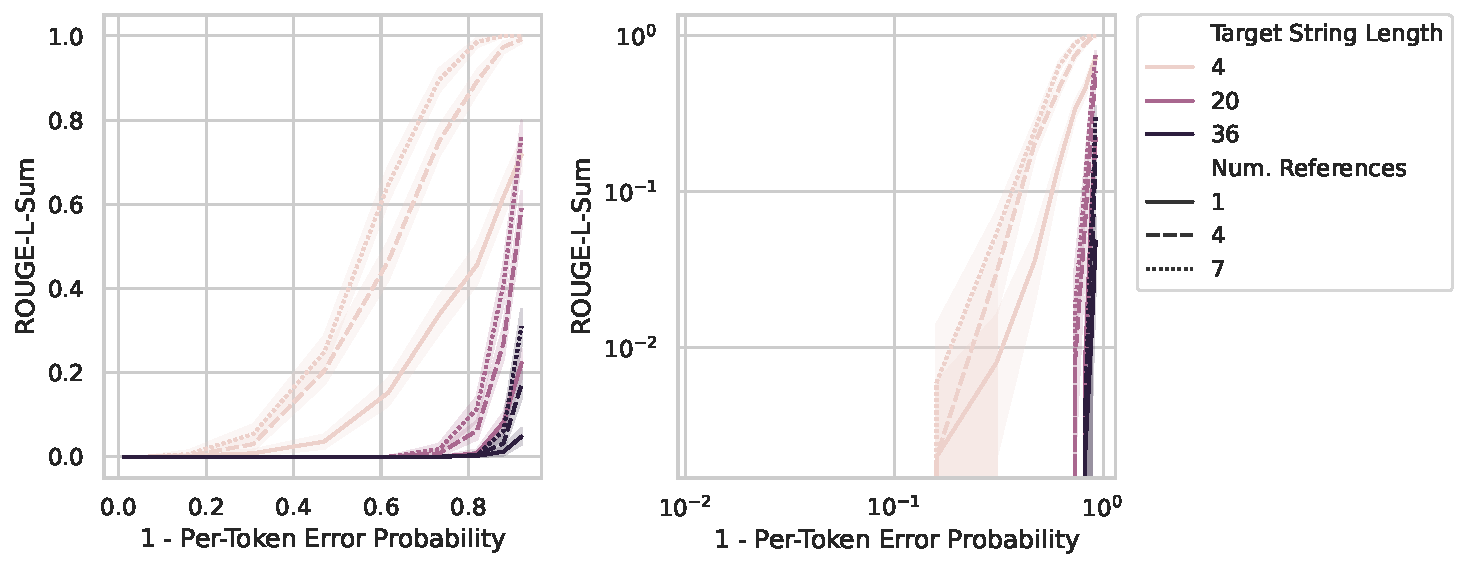
\includegraphics[width=0.95\textwidth]{figures/rouge_understanding/rougeLsum_vs_token_error_prob_scaling_simulation.pdf}
    \caption{\textbf{ROUGE-L-Sum is a sharp metric.} Simulations show that as the per-token error probability slightly increase (e.g. from 0.05 to 0.1), the ROUGE-L-Sum metric sharply falls.}
    \label{fig:app:metric_scaling:rougeLsum}
\end{figure}


Another BIG-Bench metric \cite{srivastava2022beyond} is ROUGE-L-Sum \cite{lin2004rouge}, a metric based on the longest common subsequence (LCS) between two sequences. Section 3.2 of \cite{lin2004rouge} gives the exact definition, but the key property is that ROUGE-L-Sum measures the ``union" LCS, which means ``stitching" together LCSs across the candidate and multiple references. As explained in the original paper: if the candidate sequence is $c = w_1 w_2 w_3 w_4 w_5$, and if there are two reference sequences $r_1 = w_1 w_2 w_6 w_7 w_8$ and $r_2 = w_1 w_3 w_8 w_9 w_5$, then $LCS(r_1, c) = w_1 w_2$ and $LCS(r_2, c) =w_1 w_3 w_5$, then the \textit{union} 
-LCS of $c, r_1, r_2$ is $w_1 w_2 w_3 w_5$, with length 4. Intuitively, this disproportionately benefits models with smaller error rates because their mistakes can be ``stitched" across multiple references; this is confirmed in simulation (Fig. \ref{fig:app:metric_scaling:rougeLsum}).


% \subsection{BLEU}
% \label{app:metric_scaling:bleu}


% \subsection{Emergence does not require on scaling laws: decreasing cross-entropy loss and stricter exact match is all you need }

% The goal of this section is to show that scaling laws are not necessary to create emergence and that many functional forms of the loss are valid as long as the form decreases as some other variable decreases -- say the number of parameters in the model.
% This typically holds in modern machine learning. 
% We do this by considering different functional forms of the cross entropy $CE(N)$, as a function of the number of parameters $N$, and show emergence, i.e. sharpness and unpredictability.
% We illustrate this by showing the programmer can exaggerate the sharpness (and therefore emergence) by implying increasing the exact number of tokens required to get correct in the accuracy, i.e. increasing $L$ in our notation.

% \subsubsection{Argument}

% Recall from section \ref{sec:alt_explanation} the accuracy requiring all $L$ tokens to be correct for a model of size $N$ as a function of cross-entropy $CE(N)$:

% \begin{equation*}
%     \text{Accuracy}(N) \approx p_N(\text{single token correct})^{\text{num. of tokens}} = \exp \Big(- CE(N) \Big)^L
% \end{equation*}

% We plot this equation using three functional forms for a decreasing cross-entropy loss in figure \ref{fig:decreasing_loss_leads_to_emergence_as_L_increases} for increasing values of $L$.
% These increasing values of $L$ induce a sharper -- therefore, seemingly more emergent curve when plotting the accuracy. 
% This means that if the programmer simply requires a stricter accuracy, he can make a perfectly smooth and predictable cross-entropy loss suddenly become sharp and unpredictable, i.e. ``emergent". 
% We show numerically it is independent of the functional form and instead that it only requires the cross-entropy to be decreasing and the accuracy metric to have some non-linear transformation that makes it sharper. 
% Therefore, if one had only tracked the cross-entropy loss instead, one could have had a smooth predictable curve for the models.
% This implies small-scale experimentation is still relevant, and we wish to highly that GPT-4 \cite{gpt4} small-scale experiment in conjunction with scaling loss. 
% We'd like to emphasize that changing the evaluation metric can suddenly induce emergence, and it is not an intrinsic property of the model. 

% %The goal will be to show that if $CE(N)$ decreases with different functional forms that $acc$ is emergent (either sharp or unpredictable).
% % TODO: sharp due to L
% % TODO: unpredictable due to constant and L

% \begin{figure}[htbp]
%   \centering
%   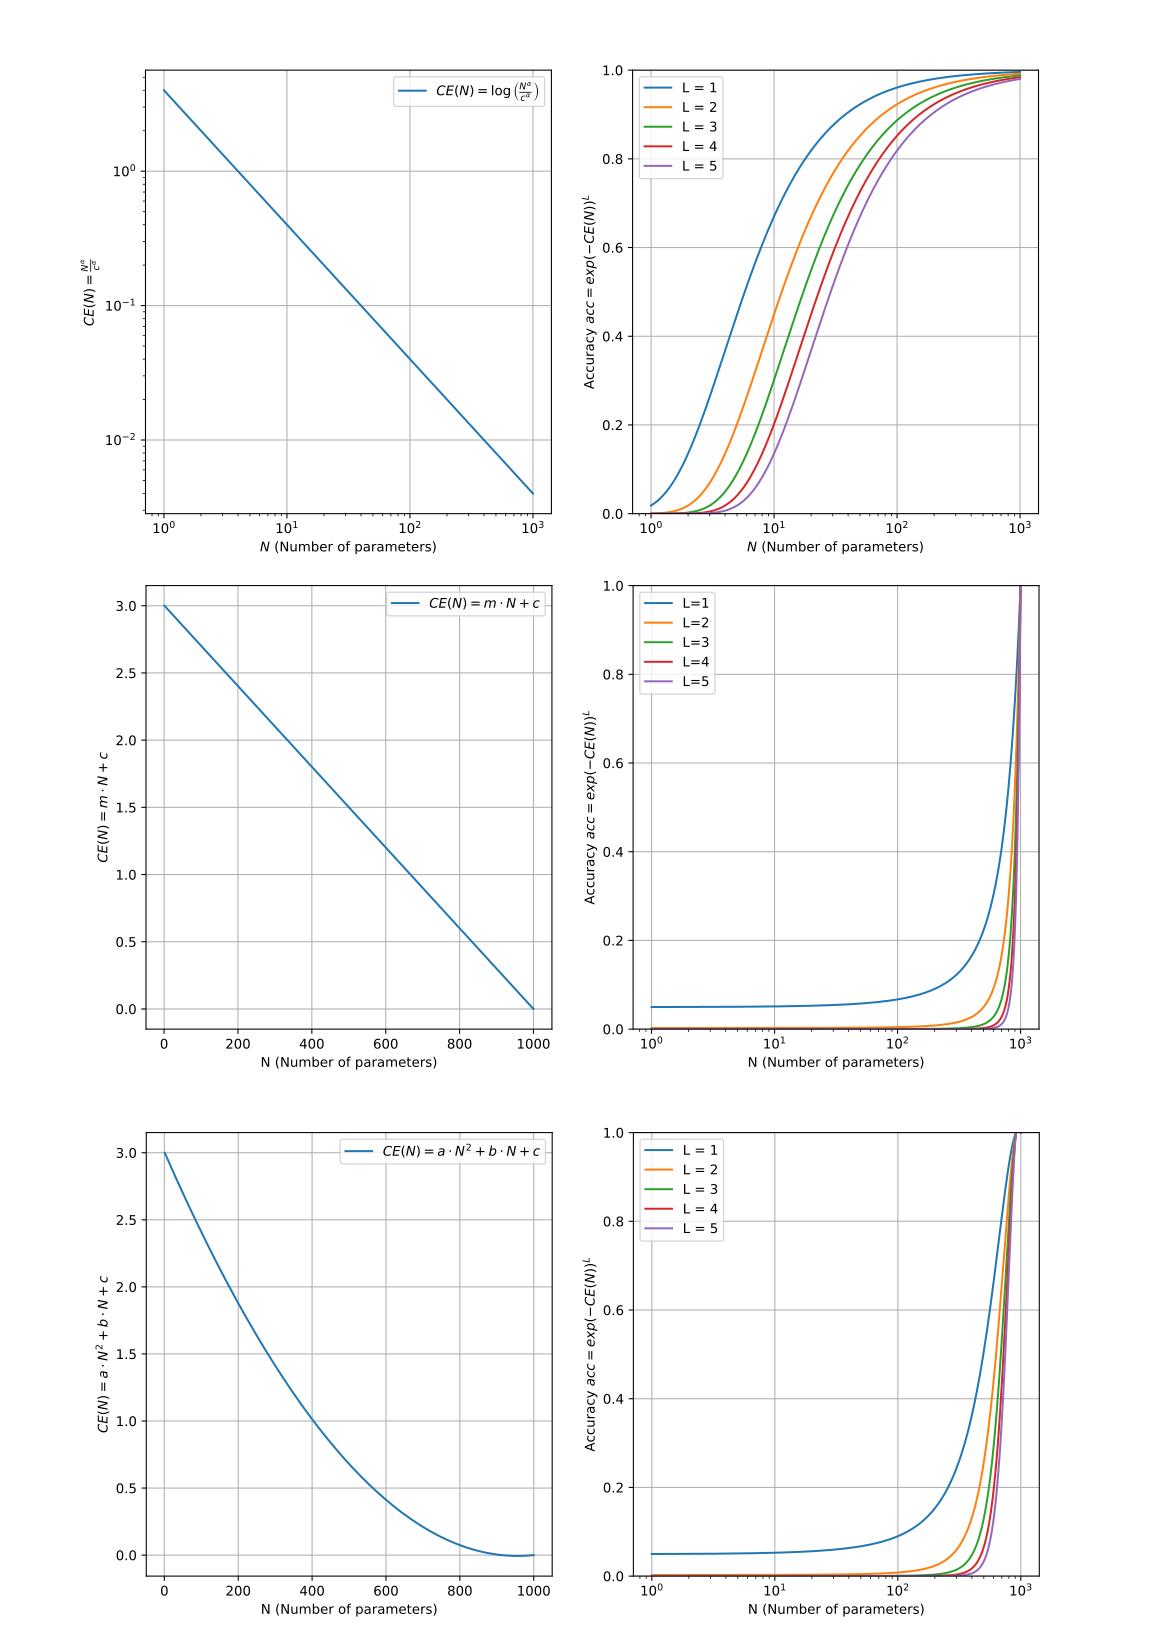
\includegraphics[width=0.8\textwidth]{figures/loss_decreasing_leads_to_emergence/decreasing_loss_leads_to_emergence_as_L_increases.png}
%   \caption{
%   \textbf{Emergence does not depend on scaling laws: any decreasing cross-entropy loss induces apparent emergence as L increases as you require more tokens to be exactly correct, i.e. L increases.}
%   The first row shows the same argument as in the main section, where a decreasing cross-entropy loss as a scaling law induces emergence as $L$ increases.
%   The second row shows the that apparent emergence is induced even when the cross-entropy loss decreases linearly.
%   The third row shows that the apparent emergence is induced when the cross-entropy loss decreases quadratically.
%   Emergence is amplified in this case especially by the increase in sharpness as more tokens are required to be correct. 
%   This means that simply changing the evaluation metric can suddenly induce emergence, and it is not an intrinsic property of the model. 
%   }
%   \label{fig:decreasing_loss_leads_to_emergence_as_L_increases}
% \end{figure}


\section{Inducing Emergent Abilities in Networks on Vision Tasks}
\label{app:sec:inducing_emergence_vision}

\subsection{Emergent Classification of MNIST Handwritten Digits by Convolutional Networks}

\begin{figure}
    \centering
    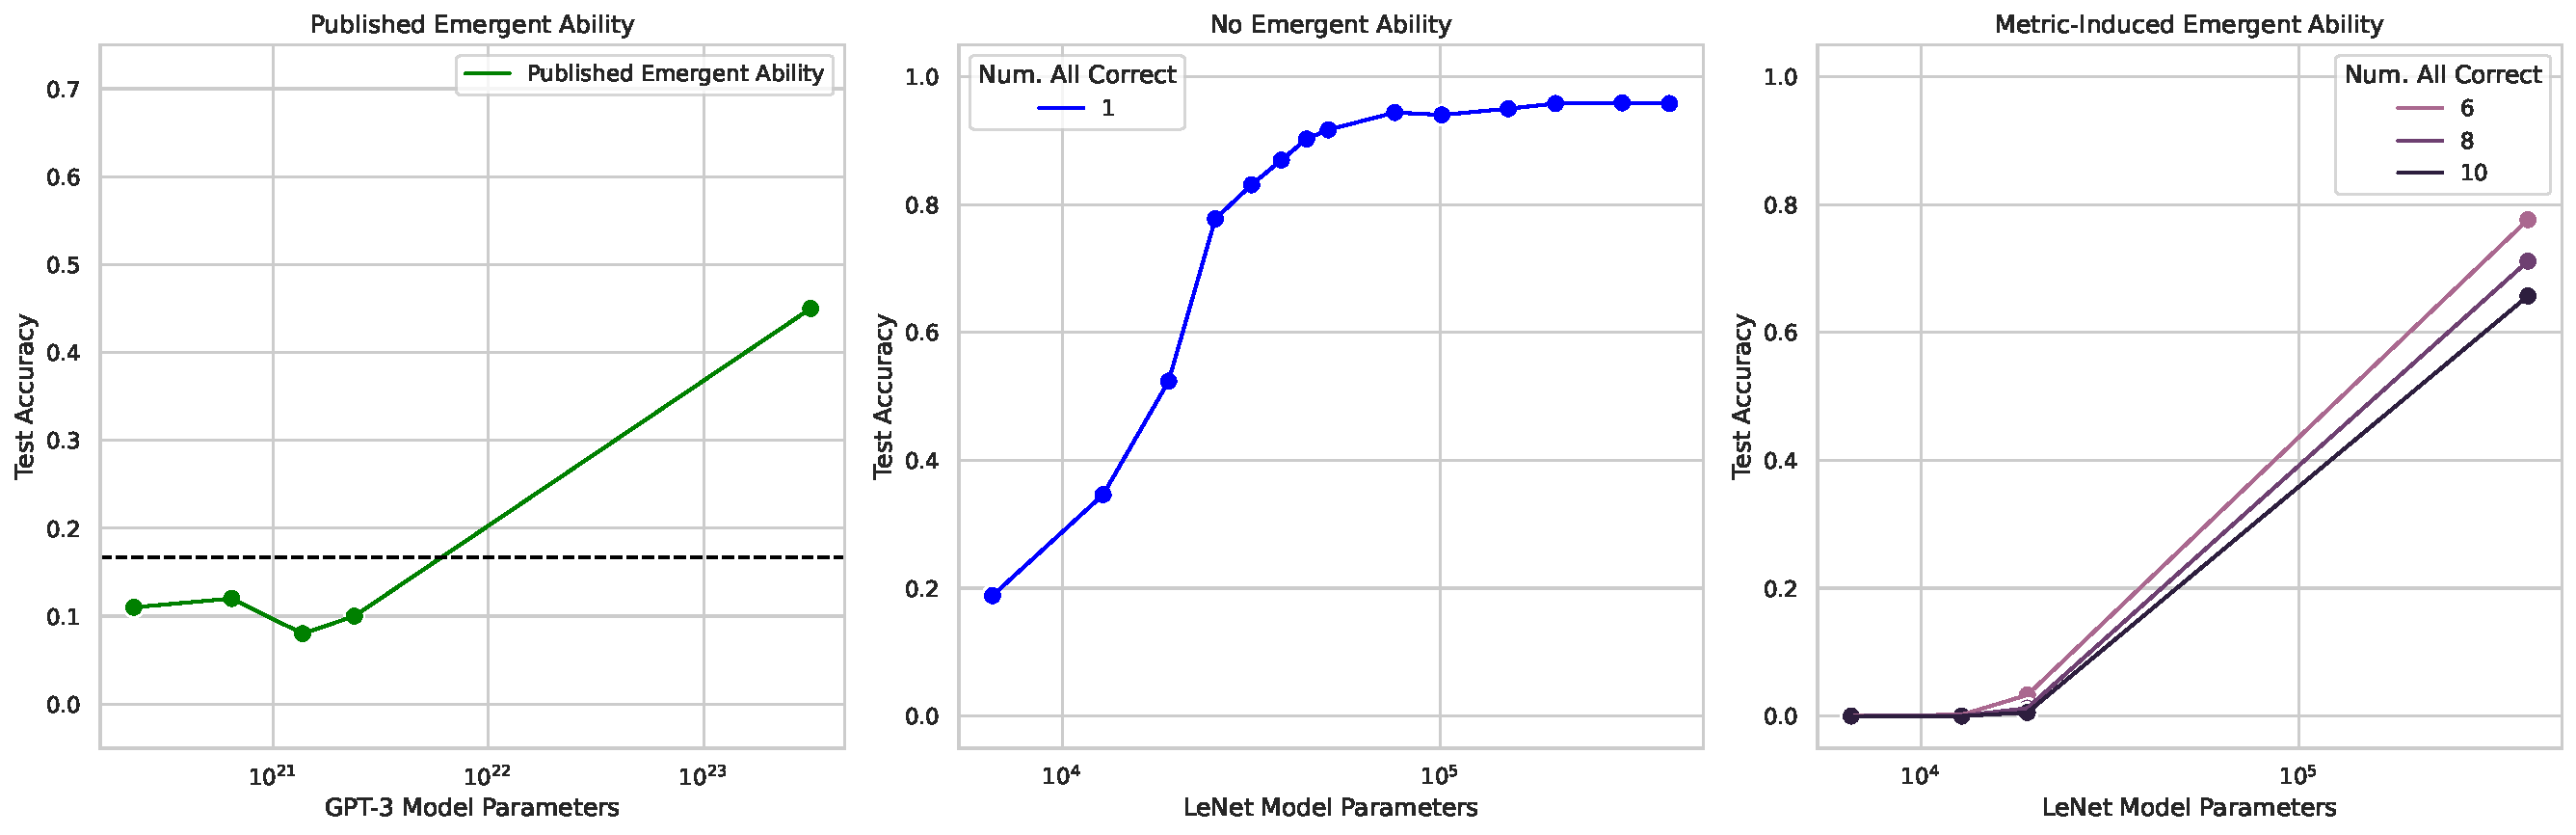
\includegraphics[width=\textwidth]{figures/vision/no_emergence_and_emergence_dataset=mnist.pdf}
    \caption{\textbf{Induced emergent MNIST classification ability in convolutional networks.} (A) A published emergent ability from the BIG-Bench Grounded Mappings task \cite{wei2022emergent}. (B) LeNet trained on MNIST \cite{lecun1998mnist} displays a predictable, commonplace sigmoidal increase in test accuracy as model parameters increase. (C) When accuracy is redefined as correctly classifying $K$ out of $K$ independent test data, this newly defined metric induces a seemingly unpredictable change.}
    \label{fig:vision_mnist}
\end{figure}

We begin by inducing an emergent classification ability in a LeNet convolutional neural network family \cite{lecun1998gradient}, trained on the MNIST handwritten digits dataset \cite{lecun1998mnist}.
This family displays smoothly increasing test accuracy as the number of parameters increase (Fig. \ref{fig:vision_mnist}B).
To emulate the accuracy metric used by emergence papers \cite{ganguli2022predictability, wei2022emergent, srivastava2022beyond}, we use \textit{subset accuracy}: 1 if the network classifies $K$ out of $K$ (independent) test data correctly, 0 otherwise.
Under this definition of accuracy, the model family displays an ``emergent" ability to correctly classify sets of MNIST digits as $K$ increases from $1$ to $5$, especially when combined with sparse sampling of model sizes (Fig. \ref{fig:vision_mnist}C).
This convolutional family's emergent classification ability qualitatively matches published emergent abilities, e.g., at the BIG-Bench Grounded Mappings task \cite{wei2022emergent} (Fig. \ref{fig:vision_mnist}A).





%TC:endignore
\end{document}
\endinput












%%
%% End of file `sample-authordraft.tex'.
